\chapter[Energy based safe control]{Energy based control for safe human-robot physical interaction}
\label{chap:safety}
\setfigurepath{figures/Safety}
%=========================================================================
\begin{synopsis}
%In this chapter, we propose physically meaningful energy related safety indicators for robots sharing their workspace with humans.
%Based on these indicators, safety criteria are introduced as constraints in
%the control algorithm. The first constraint depending on the distance between the robot and a nearby human operator is used to limit the amount of kinetic energy dissipated in case of a collision. After the establishment of physical contact, the second
%constraint is used to modulate contact forces by limiting the amount of potential energy generated within the human-robot system. The control algorithm
%is formulated as an optimization problem and computes every time-step
%the needed actuation torques for a KUKA LWR4 manipulator given some task to
%be performed, the introduced constraints and the physical limitations of
%the system to cope with. The overall framework allows a human operator
%to safely enter the workspace of the robot and physically interact with it.
In this chapter, we propose physically meaningful energy related safety indicators for robots sharing their workspace with humans.
Based on these indicators, safety criteria that bound the dynamics of the robot during interactions with its environment are introduced as constraints in the control scheme. A first constraint that depends on the real-time distance between the robot and a nearby obstacle is used to limit the amount of kinetic energy dissipated in case of a collision. After the establishment of physical-contact, a second constraint is used to modulate the contact forces by limiting the amount of equivalent energy that accumulates in the controller of the robot. The controller
is formulated as an optimization problem and computes every time-step
the needed actuation torques for a KUKA LWR4 robotic manipulator given some task to
be performed in Cartesian space, the introduced safety related constraints and the physical limitations of the system to cope with. The overall framework tested in simulation allows the robot to safely interact with its environment.
\end{synopsis}
%=========================================================================
%=========================================================================
\section{Introduction}
\label{sec:Problem statement}
Service and intervention robotics, as well as more traditional industrial robotics applications, are evolving in a direction where the workspace of the robot is very likely to be shared with humans. This may induce deliberate\footnote{For example if the robot can be both used in an autonomous mode or in a co-manipulation mode.} and non-intentional physical interactions. Safety in this context becomes a critical issue to be dealt with \cite{alami2006safe}.

To ensure safe human-robot interactions, several approaches have been explored in the robotics literature. At the hardware level, the mechanical design can be optimized to reduce the apparent inertia of the robot \cite{zinn2004} and compliant components can be introduced to allow smoother contacts and less severe impacts \cite{haddadin2012}. Torque sensing at the joint level also provides a way to actively control the impedance of the robot. The Kuka-DLR lightweight robot \cite{bischoff2010kuka}, \cite{loughlin2007dlr}, \cite{hirzinger2001} has been specifically designed to meet these challenges.

%Different control approaches using internal and external force/torque sensors have been developed to handle safety during pre and post impact/contact phases \cite{ebert2002safe}, \cite{lumelsky1993real}, \cite{ikuta2003safety}. Haddadin in \cite{haddadin2008collision} and De Luca in \cite{de2006collision} present different strategies to reduce the effect of undesired impacts. A collision detection parameter based on the estimated external torque is introduced and used to scale down the link inertia obtaining a ``lighter" robot that ``flees" from the collision area. An other strategy is to use the disturbance input to slow the robot until zero velocity then pushing it back along its original path. Heizmann and Zelinsky in \cite{heinzmann2003quantitative} propose a safety criterion based on the \textit{potential impact force} to filter the control torque of the system. The introduced controller scheme allows one to  consider two potential contact points at the same time for a real-time implementation.
%As the degree of potential injury is directly related to the mass and velocity of the colliding objects, the controller proposed in \cite{haddadin2012truly} takes into account the reflected robot inertia along a collision direction to decide about the maximum operational point velocity. The bounds on this velocity are based on experimental results relating mass, velocity, geometry and medically observable soft tissue injury by systematic drop-testing experiments with pig abdominal wall sample.
%By making use of the redundancy property of a KUKA/DLR lightweight arm, \cite{de2008exploiting} proposes a physical interaction strategy that is able to react safely to collisions while continuing to execute as much possible of the original task.
\begin{figure}[t]
\centering
\frame{
\includegraphics[width=0.5\columnwidth]{\figurepath/experiment}}
\caption{View of a user sharing the same workspace with a KUKA LWR4 robotic manipulator. The kinetic energy of the robot is modulated as function of the real-time distance between the human and the robot in order to best perform the task of the robot while ensuring safety.} 
\label{fig:experiment}
\end{figure}
%Standardized maximum values for the amount of kinetic energy  allowed to be dissipated during a collision between a robot and a nearby human are provided in the latest ISO/TS 15066 \cite{ISO15066PDF} standard. 
At the control level, a safe human-robot interaction requires: i) switching between different control modes (before/after physical contact) without causing potentially harmful discontinuities in the movements of the robot; ii) the formulation of safety indicators to reflect the amount of danger towards a considered nearby human-operator. These safety indicators must be related to the  impact and contact forces generated during physical interaction; iii) the formulation of safety criteria representing the bounds on the dynamic behaviour of the robot and finally, to be easily accounted for, the possibility to express these safety indicators and criteria as constraints related to the control input of the robot. 

The most generic way to take into account the different \textit{injury related parameters} (e.g., the impact and contact forces) for synthesising the needed safety indicators is to use an energy-based formulation of the safety problem. Indeed, energy is universal and can describe all the dangerous phenomena occurring during human-robot interaction. The impact force for example is directly caused by the amount of kinetic energy dissipated in case of a collision. This kinetic energy includes the velocity and equivalent mass data of both the robot and the human-operator. Contact forces on the other hand, derive from the amount of equivalent energy that accumulates in the controller of the robot during physical contact. And when contact is released, the risk of injury that can be caused by a fast transformation of the equivalent energy accumulated in the controller into kinetic one can also be monitored and reduced by modulating the energy of the robot.

Kinetic energy displayed by a robot during its movement has already been discussed in \cite{haddadin2008collision} and \cite{haddadin2012truly} as a good representation of the risk of injury in case of a collision with a nearby human. Also, maximum values for this property considered to be safe in case of an impact are available in the latest ISO/TS 15066 \cite{ISO15066PDF} for different regions of the human body. Unlike the various safety indicators from the literature, energy is significant during all the different interaction phases of a robot with its environment: before/after collisions, during physical contact, when the robot moves and also when it is motionless. Therefore, energy is used for the work presented in this chapter to synthesize \textit{physically meaningful} safety indicators to assess and \textit{control} the degree of danger a robotic manipulator represents when it physically interacts with its environment. These safety indicators include both the kinetic energy of the robot during its free movements and the \textit{equivalent energy} accumulated in its controller during physical contact.
%the equivalent energy accumulated in the controller of the robot during phases where physical contact between the robot and its environment is established. 

%Bottom line, for a given shape, two parameters are to be considered for safety: the impact force created at the collision instant between the robot and the human operator and the contact forces generated after the establishment of physical contact. The most generic way to include and express these parameters is to use an energetic formulation. Indeed, energy is a universal entity that can describe almost all the physical phenomena occurring during human-robot interaction. For example, the impact force is directly related to the amount of kinetic energy dissipated at the collision and the contact forces derive from the amount of potential energy generated during physical contact. 
%
%
%
During the \textit{free movements} of the KUKA LWR4 robotic arm, a safety criterion based on the maximum allowed kinetic energy for the robot is introduced  and used to constrain its dynamical behaviour in the direction of a considered obstacle\footnote{All along the manuscript, ``obstacle" is used as a generic term for any external element of the environment, e.g., a ``\textit{human-operator}". these two can be used interchangeably.} entering its workspace. This imposed constraint accounts for the dynamic capabilities (i.e., producible deceleration in operational space) of the robot and is modulated as function of the distance between the robot and the approaching obstacle. During physical contact, an other criterion based on the maximum value allowed for the \textit{equivalent energy that accumulates in the controller of the robot}\footnote{All along the manuscript, this type of energy is by \textit{abuse of language} referred to as ``\textit{potential energy}''.}, is used to modulate the contact forces between the robot and its environment. 
%
%
%
%
%
%
%
%
%
%%On the control level, the highest priority when controlling any human-friendly robot is to prevent the actions of the robot from causing any harm to the human operator. A safe human-robot interaction requires switching between different control modes (before/after physical contact) without causing harmful discontinuities in the movements of the robot. The formulation of safety indicators to reflect the amount of danger towards the human operator; These safety indicators must be related to the impact and contact forces generated during physical interaction and also to the mass of the robot. The formulation of safety criteria representing the bounds on the dynamic behaviour of the robot and finally, expressing these safety indicators and criteria as constraints related to the control parameters. 
%
%The most generic way to take into account the different parameters that must be considered for the formulation of the safety indicators is to use  energy. Indeed, energy is a universal property that can describe all the physical phenomena occurring during human-robot interaction. For example, the impact force is directly related to the amount of kinetic energy dissipated at a collision and the contact forces derive from the amount of potential energy generated during physical contact between the robot and . 
%
%Kinetic energy displayed by a robot during its movement has already been discussed in \cite{haddadin2008collision} and \cite{haddadin2012truly} as a good representation of the risk of injury in case of a collision with a nearby human. Maximum values of this property considered to be safe in case of a human-robot impact are provided in the latest ISO/TS 15066 \cite{ISO15066PDF} for different regions of the human body. 
%
%Kinetic energy is used in the work presented hereby to synthesize a physically meaningful safety indicator. This indicator can also include the equivalent energy accumulated in the controller during phases where physical contact between the robot and its environment is established. 
%
%%Bottom line, for a given shape, two parameters are to be considered for safety: the impact force created at the collision instant between the robot and the human operator and the contact forces generated after the establishment of physical contact. The most generic way to include and express these parameters is to use an energetic formulation. Indeed, energy is a universal entity that can describe almost all the physical phenomena occurring during human-robot interaction. For example, the impact force is directly related to the amount of kinetic energy dissipated at the collision and the contact forces derive from the amount of potential energy generated during physical contact. 
%
%
%
%
%The kinetic energy part of an introduced safety criteria is used to constrain the dynamical behaviour of a KUKA LWR4 serial robot in the direction of a considered obstacle\footnote{All along the manuscript, ``obstacle" is used as a generic term for any external element of the environment, \textit{e.g.} a human operator.}. The imposed constraint accounts for the braking capabilities of the robot and is modulated as a function of the distance between the robot and an operator entering its workspace.
%
%
%
%These different contributions provide an initial response to the fixed goals; However, the presence of dynamic constraints (e.g. mobile obstacles) and human operators around the robot highlight other concerns that must be dealt with. The highest priority in the control of any type of human-friendly robot is to prevent of the actions of the robot from causing any harm to the human operator. A safe human-robot collaboration requires switching between different control modes (before/after physical contact), the formulation of safety indicators to reflect the amount of danger towards the human operator, the formulation of safety criteria representing the bounds on the dynamic behaviour of the robot and finally expressing all of these as constraints related to the control parameters. Bottom line, for a given shape, two parameters are to be considered for safety: the impact force created at the collision instant between the robot and the human operator and the contact forces generated after the establishment of physical contact. The most generic way to include and express these parameters is to use an energetic formulation. Indeed, energy is a universal entity that can describe almost all the physical phenomena occurring during human-robot interaction. For example, the impact force is directly related to the amount of kinetic energy dissipated at the collision and the contact forces derive from the amount of potential energy generated during physical contact. 

In order to properly account for the introduced safety constraints, the control problem is expressed as a Linearly Constrained Quadratic Program (LQP) \cite{boyd2004}. The computation of the adequate actuation torque needed to perform a trajectory tracking in operational space is subject to several linear inequality constraints accounting for the physical limitations of the robot (joint limits, joint velocity, torque and jerk saturations) as well as for the limit values of the energy-based safety indicators. 

Finally, thanks to the constraint on the kinetic energy of the robot during its free movements, the proposed control framework is expected to decrease the impact forces at collisions. Contact forces on the other hand, are saturated through the constraint on the \textit{equivalent energy} that accumulates in the controller of the robot during physical interaction. Using the same framework, impact and contact forces can be modulated and the dynamics of the robot  controlled by a straightforward modification of the values of the safety criteria imposed to the system. Fig.~\ref{fig:experiment} illustrates a typical workspace-sharing scenario for the proposed controller.

This chapter is organised as follows: In Section~\ref{sec:inter1}, the proposed safety indicators are formulated for both the pre-collision and physical-contact phases. In Section~\ref{sec:salimval1}, the associated safety criteria, namely the maximum allowed values for the introduced safety indicators are introduced. The controller is described in Section~\ref{sec:safe_controller}: task related objectives are formulated and the energy related constraints needed for a safe human-robot interaction are expressed as function of the dynamic control input of the robot. In Section~\ref{sec:contrl12}, a test case scenario is introduced using a KUKA LWR4 serial robot in a simulated world, based on which, the possibilities offered by the proposed controller are illustrated and discussed. Finally, Section~\ref{sec:safety1conclusion} summarizes and discusses the contributions and provides an overview of the needed developments.
%=========================================================================
%=========================================================================
\section{Interaction forces and safety indicators}
\label{sec:inter1}
In this section, safety indicators quantifying the degree of danger\footnote{Risk induced by a collision or physical contact.} represented by the robot towards a nearby human-operator are introduced. These indicators must be \textit{physically meaningful} so they can satisfy the safety limits recommended by the ISO/TS 15066 standard \cite{ISO15066PDF}, related to the control input of the robot and computable in real-time. 
%During human-robot interaction, the degree of danger is mainly caused by two parameters: the impact force created in case of a collision and contact forces existing after the establishment of physical contact.
%
%The most generic way to take into account the different injury related parameters for synthesising safety indicators is to use an energetic formulation. Indeed, energy is a universal property that can describe all the dangerous phenomena occurring during human-robot interaction. The impact force for example is directly related to the amount of kinetic energy dissipated at collisions. This kinetic energy includes the inertial information of the robot. Contact forces on the other hand, derive from the amount of equivalent energy accumulated in the controller during physical contact phases. In case of contact release, the risk of injury that may be caused by a fast transformation of the equivalent energy in the controller into kinetic energy can also be monitored and reduced by modulating the robot's energy. Energy is therefore used in the presented work to synthesize two indicators whose value is related to the impact and contact forces. Safety criteria, namely bounds on the maximum values of these indicators are then derived. The energy based criteria are finally used to constrain the dynamic behaviour of a KUKA LWR4 serial robot as it physically interacts with its environment.


%During human-robot interaction, the degree of danger is mainly caused by two parameters: the impact force created in case of a collision and contact forces existing after the establishment of physical contact. The most generic way to include and express these forces is to use an energetic formulation. Indeed, energy is a universal entity that can describe all the physical phenomena occurring during human-robot interaction \footnote{Physical and non physical.}. Therefore, it is used in the presented work to synthesize two indicators whose value is related to the impact and contact forces. Safety criteria, namely bounds on the maximum values of these indicators are then derived. The energy based criteria are finally used to constrain the dynamic behaviour of a KUKA LWR4 serial robot as it physically interacts with its environment. 
%%%%%%%%%%%%%%%%%%%%%%%%%%SUBSECTION%%%%%%%%%%%%%%%%%%%%%%%%%%%%%
%%%%%%%%%%%%%%%%%%%%%%%%%%%%%%%%%%%%%%%%%%%%%%%%%%%%%%%%%%%%%%%%%
%%%%%%%%%%%%%%%%%%%%%%%%%%SUBSECTION%%%%%%%%%%%%%%%%%%%%%%%%%%%%%
\subsection{Kinetic energy}
The generated impact force in case of a collision between the robot and its environment can be written as function of the dissipated kinetic energies and the shock absorption distance:
\begin{equation}
\begin{split}
\int_u F_{impact} du  & = E_{dissipated} \\
                      & = E_{c}^{hum} + E_{c}^{rob},
\end{split}
\label{eq:Energydissipationmodel1}
\end{equation}
$ F_{impact} $ is the generated impact force at collision, $u$ the shock absorption distance and $E_{dissipated}$ the dissipated energy which is equal to the sum of kinetic energies $E_{c}$ of both the human-operator and the robot. 
On the one hand, the left side parameters of the shock absorption equation (\ref{eq:Energydissipationmodel1}) are not directly related to the actuation torque of the robot. Moreover, it is impossible to have an accurate model of the human body-robot impedance\footnote{This model would have to be individual and body-part specific.}. As a matter of fact, the use of the impact force or of the shock absorption distance as a safety indicator is neither desirable nor possible. On the other hand, the dissipated energy is closely related to the impact force and can be directly related to the actuation torque of the robot and thus, controlled in order to reduce the impact of a collision.
\\
At a given time, very few assumptions can be made on the energy-state of the nearby human-operator and on its future evolution. As a consequence, the retained safety indicator $S_c$ is robot-centred. $E_{c}^{rob}$ is directly related to the impact force and can be expressed using the control torque input. It is therefore considered for the formulation of the first safety indicator $S_c$: 
\begin{equation}
\begin{split}
S_c^{i,j} = E_{c}^{i,j} = \frac{1}{2}  m(\vect{q}_{|k})_{i,j}^{eq} v_{C}^{i,j}^2,
\end{split} 
\end{equation}
with: $1/m(\vect{q}_{|k})_{i,j}^{eq}  = J(\vect{q}_{|k})_{C}^{i,j} M(\vect{q}_{|k})^{-1} J(\vect{q}_{|k})_{C}^{{i,j}^T}$; $m(\vect{q}_{|k})_{i,j}^{eq}$ being the equivalent mass of the robot segment $i$ in the direction of obstacle $j$ expressed in the Cartesian space \cite{khatib1995inertial}. $M(\vect{q}_{|k})$ is the joint space inertia matrix of the robot and $\vect{q}_{|k}$ its joint space configuration at time-step $k$; $v_{C}^{i,j} = J(\vect{q}_{|k})_{C}^{i,j} \dot{\vect{q}}_{|k}$ is the relative linear velocity of the closest point $C$ belonging to the robot segment $i$ in the direction of obstacle $j$; $J(\vect{q}_{|k})_{C}^{i,j}$ is the Jacobian of the robot segment $i$ expressed at point $C$ and projected along the distance vector towards obstacle $j$. \\
To ensure safety for both the robot and any nearby obstacle, the introduced safety indicator must be considered for each (robot segment $i$, obstacle $j$) pair, i.e., for $N_O$ obstacles and a robot composed of $N_b$ mobile bodies, $N_O \times N_b$ safety indicators are needed. An other solution is to consider a safety indicator related to the real-time closest points $C$ and $O$ respectively on the robot and the human-operator. The main drawback with such approach is however the inevitable discontinuities that can be caused by the geometrical shapes of both the robot and the human, and that will be directly reflected on the expression of the safety indicator. \\
Within the framework of this chapter, and without loss of generality, a single obstacle $O$ is considered and the only mobile part of the robot considered for the formulation of the \textit{pre-collision} safety indicator is the end-effector (EE). Indeed, generally speaking, it is usually  the last segment of the fixed-base serial robot KUKA LWR4 that holds the practical load and that consequently deploys the maximum amount of kinetic energy in contrast with the other segments of the robot. The kinetic energy based safety indicator is then written: 
\begin{equation}
S_c = E_{c_{|k}}^{EE,O} = \frac{1}{2} m(\vect{q}_{|k})^{eq} v^2,
\label{eq:Ec_constr_first}
\end{equation}
with: $m(\vect{q}_{|k})^{eq} = m(\vect{q}_{|k})_{EE,O}^{eq}$ and $v = v_{EE}^{EE,O} = \vect{\dot{X}}_{EE_{|k}} \vect{n}_{O_{|k}}$. This indicator represents the energy that will be dissipated by the end-effector of the robot  in case of a collision with a nearby obstacle (see Fig.~\ref{fig:small_dist_rob_obst}).
\begin{figure}[H]
\captionsetup{width=1\linewidth}
\centering

\includegraphics[width=0.52\linewidth]{\figurepath/obstacle_nobackground}
\caption{The closest distance $d$ between the end-effector of the robot $EE$ and an obstacle $O$ entering its workspace.}
\label{fig:small_dist_rob_obst}
\end{figure}
%%%%%%%%%%%%%%%%%%%%%%%%%%SUBSECTION%%%%%%%%%%%%%%%%%%%%%%%%%%%%%
%%%%%%%%%%%%%%%%%%%%%%%%%%%%%%%%%%%%%%%%%%%%%%%%%%%%%%%%%%%%%%%%%
%%%%%%%%%%%%%%%%%%%%%%%%%%SUBSECTION%%%%%%%%%%%%%%%%%%%%%%%%%%%%%
\subsection{Potential energy}
When physical contact between the robotic manipulator and an obstacle in its environment is established at a contact point $C$, the resulting contact force is created as a consequence of the amount of energy that accumulates in the controller of the robot. The instantaneous force $F_{C_{|k}}$ that pulls the contact point $C$ in the direction of its desired position\footnote{Considering a trajectory tracking task.} in operational space is derived from the controller's energy $E_{p_{|k}}$:
\begin{equation}
F_{C_{|k}} = -\vect{\nabla} E_{p_{|k}}.
\label{eq:F_drved_Ep}
\end{equation}
Therefore:
\begin{equation}
E_{p_{|k}} = -\int_{\vect{X}_{C_{|k}}^{*}}^{\vect{X}_{C_{|k}}} F_{C_{|k}} d\vect{x} = \int_{\vect{X}_{C_{|k}}}^{\vect{X}_{C_{|k}}^{*}} F_{C_{|k}} d\vect{x} = F_{C_{|k}} \left(\vect{X}_{C_{|k}}^{*} - \vect{X}_{C_{|k}}\right) \vect{n}_{C_{|k}},
\label{eq:Ep_is_force_int}
\end{equation}
with:
\begin{equation}
\begin{split}
F_{C_{|k}} = m(\vect{q}_{|k})_{C,C^*}^{eq} \ddot{X}_{C_{|k}},
\end{split}
\label{eq:expl_F_meq}
\end{equation}
$\vect{n}_{C_{|k}}$ represents the instantaneous directing vector between the contact point $C$ (on the considered segment $i$) and its desired position $C^*$ (see Fig.~\ref{fig:small_dist_rob_obst2}). \\
$\ddot{X}_{C_{|k}} = \left(\dot{J}(\vect{q}_{|k})_{C} \vect{\dot{q}}_{|k} + J(\vect{q}_{|k})_{C} \vect{\ddot{q}}_{|k}^{c}\right) \vect{n}_{C_{|k}}$ is the Cartesian acceleration of the contact point $C$ along the $C,C^*$ instantaneous distance vector $\vect{n}_{C_{|k}}$ and $\vect{\ddot{q}}_{|k}^{c}$ is the dynamic acceleration control variable that corresponds to the control torque input $\vect{\tau}_{|k}^{c}$ (considering a dynamic controller). 

Depending on the type of controller used to track the desired trajectory for the robot in operational space, the contact force applied by the robot to its environment when its movement is restrained during physical contact can be either \textit{conservative} or \textit{non-conservative}. For example, in case of a purely  proportional controller ($K_p~\Delta X$), the amount of energy that accumulates in the controller of the robot depends on the instantaneous real and desired positions ($\vect{X}_{C_{|k}}$ and $\vect{X}_{C_{|k}}^{*}$) of the contact point $C$. The nature  of the controller's energy in this case is similar to a \textit{potential energy} stored into a compressed physical mechanical spring. However, when different control schemes are used, for example, a proportional derivative controller ($K_p~\Delta X + K_d~\Delta \dot{X}$) or a complete PID with a feed-forward term, \textit{non-conservative} forces that participate in the traction\footnote{Note that this traction does not result in any movement of the robot's contacted area, static contact is considered.} of the contact point $C$ during physical interaction are added. The energy that accumulates in the controller of the robot in such case is partially \textit{path dependent} and does not \textit{exclusively} depend on the instantaneous real and desired positions of the robot's contact point $C$. \\
On the other hand, the equivalent force \textit{virtually pulling the robot} that results from any type of controller that is adapted for trajectory tracking, will\footnote{Tracking errors aside.} always make the real position of the robot $\vect{X}_{C_{|k}}$ ultimately converge towards its desired position $\vect{X}_{C_{|k}}^*$. The work carried out even by a non or only partially conservative force will always be between the two positions: $\vect{X}_{C_{|k}}$ and $\vect{X}_{C_{|k}}^*$. Which are therefore used for the formulation of the amount of energy that accumulates in the controller of the robot during physical contact (\ref{eq:Ep_is_force_int}). For convenience, and even if the equivalent energy of the controller during physical contact is not always linked to a fully conservative force, in the upcoming sections, this energy can be \textit{by abuse of language} referred to as \textit{potential energy}.     

$E_{p_{|k}}$ is directly related to the contact force generated during physical contact and can be expressed using the dynamic actuation variables (articular acceleration/torque $[\vect{\ddot{q}}_{|k}^{c}, \vect{\tau}_{|k}^{c}]$). It is therefore used for the formulation of the safety indicator that reflects the degree of danger of the robot during physical interaction phases. Finally, the retained safety indicator $S_{p_{contact}}$ is robot centred and can be written:
\begin{equation}
S_{p_{contact}} = E_{p_{|k}} = F_{C_{|k}} \left(\vect{X}_{C_{|k}}^{*} - \vect{X}_{C_{|k}}\right) \vect{n}_{C_{|k}}.
\end{equation}
In case of a physical contact that occurs at the level of the end-effector of the robot (EE) (see Fig.~\ref{fig:small_dist_rob_obst2}), $S_{p_{contact}}$ can be written:   
\vspace{-1 mm}
\begin{equation}
\begin{split}
S_{p_{contact}} = E_{p_{|k}}^{EE,EE^*} &= F_{EE_{|k}}\left(\vect{X}_{EE_{|k}}^{*} - \vect{X}_{EE_{|k}}\right) \vect{n}_{EE_{|k}} ,
\\
&= m(\vect{q})_{EE,EE^*}^{eq} \ddot{X}_{EE_{|k}} \left(\vect{X}_{EE_{|k}}^{*} - \vect{X}_{EE_{|k}}\right) \vect{n}_{EE_{|k}}.
\end{split}
\label{eq:Ep_constr_221}
\end{equation}
\vspace{-5mm}
\begin{figure}[H]
\captionsetup{width=1\linewidth}
\centering
\includegraphics[width=0.59\linewidth]{\figurepath/obstacle_nobackground2}
\caption{Instantaneous force $\vect{F}_{EE_{|k}}$ applied by a robotic manipulator to an obstacle in its environment. The contact point $C$ in this case is the point $EE$ of the end-effector of the robot.}
\label{fig:small_dist_rob_obst2}
\end{figure}
\vspace{-1mm}
Finally, $S_{p_{contact}}$ represents the amount of potential energy that accumulates in the controller of the robot during a physical contact with its environment. This same potential energy, in case physical contact is released is to be transformed into kinetic one as the robot catches its desired position.
%%%%%%%%%%%%%%%%%%%%%%%%%%SUBSECTION%%%%%%%%%%%%%%%%%%%%%%%%%%%%%
%%%%%%%%%%%%%%%%%%%%%%%%%%%%%%%%%%%%%%%%%%%%%%%%%%%%%%%%%%%%%%%%%
%%%%%%%%%%%%%%%%%%%%%%%%%%SUBSECTION%%%%%%%%%%%%%%%%%%%%%%%%%%%%%
\subsection{Relation between kinetic and potential energies}
\label{subsec:relEcEp}
During \textit{free movements}\footnote{Movements without any physical interaction with the environment.} of the robot, the equivalent force: 
\begin{equation}
F_{C_{|k}} = m(\vect{q}_{|k})_{C_{|k},C_{|k+1}}^{eq} \ddot{X}_{C_{|k}},
\label{eq:pulling_force}
\end{equation}
derived from the potential energy $E_{p_{|k}}$, pulls the potential collision point $C$ along its desired trajectory from its current position $\vect{X}_{C_{|k}}$ to its future position $\vect{X}_{C_{|k+1}}$. $E_{p_{|k}}$ results from feeding the 
desired Cartesian position, velocity and feed-forward acceleration\footnote{We consider a trajectory tracking task in Cartesian space. The desired position, velocity and feed-forward acceleration are generated using a trajectory generator.} to the controller of the robot. During these movements, Newton's third law of motion is satisfied. It can be written:
%\begin{equation}
%2 \hspace{0.5mm} \textnormal{sign(}  \vect{\ddot{X}}_{C_{|k}} \textnormal{)} \footnote{Positive towards the obstacle and negative in the opposite direction.} \hspace{0.5mm} \left\| \vect{\ddot{X}}_{C_{|k}} \right\| \left\| \vect{X}_{C_{|k+1}} - \vect{X}_{C_{|k}} \right\|_{C,*} = v_{C_{|k+1}}^2 - v_{C_{|k}}^2
%\label{eq:2pts_mvt_dyn21}
%\end{equation}
\begin{equation}
2 \ddot{X}_{C_{|k}} \left(\vect{X}_{C_{|k+1}} - \vect{X}_{C_{|k}}\right) \vect{n}_{C_{|k}} = v_{C_{|k+1}}^2 - v_{C_{|k}}^2,
\label{eq:2pts_mvt_dyn21}
\end{equation}
$v_{C_{|k+1}}$ and $v_{C_{|k}}$ are respectively the current and future Cartesian velocities of the robot expressed at the potential collision point $C$. Multiplying both sides of (\ref{eq:2pts_mvt_dyn21}) by $\dfrac{1}{2} m(\vect{q})_{C_{|k},C_{|k+1}}^{eq}$ results in: 
%\begin{equation}
%\textnormal{sign(}  \vect{\ddot{X}}_{C_{|k}} \textnormal{)} m(\vect{q})_{C,*}^{eq} \left\| \vect{\ddot{X}}_{C_{|k}} \right\| \left\| \vect{X}_{C_{|k+1}} - \vect{X}_{C_{|k}} \right\|_{C,*} = \frac{1}{2} m(\vect{q})_{C,*}^{eq} (v_{C_{|k+1}}^2 - v_{C_{|k}}^2)
%\label{eq:Ec_var_eq_Ep}
%\end{equation}
\begin{equation}
m(\vect{q}_{|k})_{C_{|k},C_{|k+1}}^{eq} \ddot{X}_{C_{|k}} \left(\vect{X}_{C_{|k+1}} - \vect{X}_{C_{|k}}\right) \vect{n}_{C_{|k}} = \frac{1}{2} m(\vect{q}_{|k})_{C_{|k},C_{|k+1}}^{eq} \left(v_{C_{|k+1}}^2 - v_{C_{|k}}^2\right),
\label{eq:Ec_var_eq_Ep}
\end{equation}
which is equivalent to:
\begin{equation}
E_{p_{|k}}^{C_{|k},C_{|k+1}} = E_{c_{|k+1}}^{C_{|k},C_{|k+1}} - E_{c_{|k}}^{C_{|k},C_{|k+1}} \Leftrightarrow E_{c_{|k+1}}^{C_{|k},C_{|k+1}} = E_{c_{|k}}^{C_{|k},C_{|k+1}} + E_{p_{|k}}^{C_{|k},C_{|k+1}}.
\label{eq:Ec_var_eq_Ep2}
\end{equation} 
%\vect{\ddot{q}}_{|k}^{c}
Meaning that, the kinetic energy $E_{c_{|k+1}}^{C_{|k},C_{|k+1}}$ of the robot expressed at the potential collision point $C$ at time-step $k+1$ is equal to its kinetic energy at time-step $k$ plus the \textit{injected} potential energy $E_{p_{|k}}^{C_{|k},C_{|k+1}}$; that represents the equivalent energy instantaneously injected in the controller of the robot along the $\vect{n}_{C_{|k}}$ vector (see Fig.~\ref{fig:small_dist_rob_obst33}). This energy makes the potential collision point $C$ move from its initial position $\vect_{X}_{C_{|k}}$ to its next position $\vect_{X}_{C_{|k+1}}$. $\ddot{X}_{C_{|k}} = \left(\dot{J}(\vect{q}_{|k})_{C} \vect{\dot{q}}_{|k} + J(\vect{q}_{|k})_{C} \vect{\ddot{q}}_{|k}^{c}\right) \vect{n}_{C_{|k}}$ is the acceleration of the potential collision point in operational space.
\begin{figure}[H]
\captionsetup{width=1\linewidth}
\centering
\includegraphics[width=0.50\linewidth]{\figurepath/rob_nobackground33}
\caption{Equivalent force $\vect{F}_{C_{|k}}$ expressed at the potential collision point $C$ pulling a robotic arm towards its desired trajectory from its current position $\vect{X}_{|k}$ to its future position $\vect{X}_{|k+1}$. The potential collision point $C$ in this case is the end-effector point $EE$.}
\label{fig:small_dist_rob_obst33}
\end{figure}
\vspace{-1mm}
%$\left\|\vect{A}\right\|_{i,j}$ is the norm of vector $\vect{A}$ projected along the $i,j$ direction. 
According to (\ref{eq:Ec_var_eq_Ep2}), the \textit{injected} potential energy $E_{p_{|k}}^{C_{|k},C_{|k+1}}$, when released, modifies the kinetic energy of the robot in the right direction to accomplish the trajectory tracking task. Therefore, the kinetic energy of the system $E_{c_{|n}}$ at a given time-step $k = n$ can be expressed as the sum of all the previously injected potential energies $E_{p_{|n}}$: 
\begin{equation}
E_{c_{|k}} = \sum\limits_{n=1}^{k-1} E_{p_{|n}}.
\label{eq:Ec_eq_sum_Ep_a}
\end{equation}
As the desired trajectory for the end-effector is discretized, every time step, only a small amount of potential energy $E_{p_{|k}}$ is \textit{injected} then promptly transformed into kinetic one as the robot moves. The modulation of this \textit{injected} potential energy can then directly influence the resulting kinetic energy of the robot and therefore the impact force $\vect{F}_{impact}$ in case of a collision. Thus, the instantaneously injected potential energy in the controller of the robot before collision can also be used as a safety indicator during its \textit{free} movements. When expressed at the level of the end-effector $(EE)$, the injected potential energy in the direction of a considered obstacle $O$ is written:
%The injected potential energy at the level of the end-effector in the direction of a considered obstacle $O$ can be expressed:
\begin{equation}
S_{p_{free}} = E_{p_{|k}}^{EE,O} = m(\vect{q}_{|k})_{EE,O}^{eq} \ddot{X}_{EE_{|k}}^{EE,O} \left(\vect{X}_{EE_{|k+1}} - \vect{X}_{EE_{|k}}\right) \vect{n}_{O_{|k}}.
\label{eq:Sp_free_mvts}
\end{equation}
$\vect{n}_{O_{|k}}$ is the unitary vector that corresponds to the distance between the end-effector of the robot (EE) and the closest point from a considered nearby obstacle $O$ (see Fig.~\ref{fig:small_dist_rob_obst}). Notice that the expression of this \textit{potential energy based safety indicator} during the \textit{free} movements of the robot is different from the expression of the safety indicator $S_{p_{contact}}$ previously proposed for the physical contact phases (\ref{eq:Ep_constr_221}). Indeed, the two points in Cartesian space between which the two \textit{potential energy base safety indicators} $S_{p_{contact}}$ and $S_{p_{free}}$ are considered, are different. For $S_{p_{contact}}$, the potential energy that accumulates in the controller of the robot during physical contact is considered between the instantaneous real position of its end-effector $\vect{X}_{EE_{|k}}$ and the desired position $\vect{X}_{EE_{|k}}^*$. Indeed, the contact force that derives from $S_{p_{contact}}$ during such phase depends directly on the distance $\left(\vect{X}_{EE_{|k}}^*-\vect{X}_{EE_{|k}}\right)$. On the other hand, for $S_{p_{free}}$, during \textit{free} movements of the robot, the potential energy instantaneously \textit{injected} in the controller of the robot modifies the kinetic energy expressed at its end-effector between its current  position $\vect{X}_{EE_{|k}}$ and its position $\vect{X}_{EE_{|k+1}}$ at the next time-step. Because of tracking errors that increase particularly when coping with constraints, the end-effector of the robot \textit{practically} never reaches exactly its imposed desired position $\vect{X}_{EE_{|k}}^*$ at time-step $k+1$.  $\vect{X}_{EE_{|k+1}}$ is therefore \textit{practically} never equal to $\vect{X}_{EE_{|k}}^*$. Instead of $\left(\vect{X}_{EE_{|k}}^*-\vect{X}_{EE_{|k}}\right)$, the distance between $\vect{X}_{EE_{|k}}$ and $\vect{X}_{EE_{|k+1}}$ is therefore used for the expression of the second formulation (\ref{eq:Sp_free_mvts}) of the pre-collision safety indicator $S_c$ during the \textit{free} movements of the robot.
%=========================================================================
%=========================================================================
\section{Safety limit values}
\label{sec:salimval1}
In this section, safety criteria that bound the energy-based safety indicators previously presented are formulated. The introduced safety indicators together with the safety criteria will then be used to formulate the proper constraints on the energy, the robot is allowed to display during interaction with its environment.
%%%%%%%%%%%%%%%%%%%%%%%%%%SUBSECTION%%%%%%%%%%%%%%%%%%%%%%%%%%%%%
%%%%%%%%%%%%%%%%%%%%%%%%%%%%%%%%%%%%%%%%%%%%%%%%%%%%%%%%%%%%%%%%%
%%%%%%%%%%%%%%%%%%%%%%%%%%SUBSECTION%%%%%%%%%%%%%%%%%%%%%%%%%%%%%
\subsection{Safety limit value for the pre-collision safety indicator}
For $S_c$ , the safety criterion represents
the maximum amount $E_{c_{limit}}$ of kinetic energy allowed to be dissipated in case of a collision between the robot and a human within its workspace. The first safety constraint can be written: $S_c \leq E_{c_{limit}}$ and must be satisfied at every time-step during the movements of the robot. Given the nature of $S_c$, such constraint when imposed at the control level, may have two consequences: a limitation of the end-effector's velocity in direction of the considered obstacle and a modification of its apparent mass along the same direction. However, when no human is at a close distance from the robot, it becomes unnecessary to saturate its kinetic energy of the robot as it accomplishes its task. \\
Therefore, to prevent over-limiting the dynamics of
the system without needed cause, the reaction of the robot towards a nearby obstacle can be as follows: when the human is far from the robot, the system can be as dynamic as possible to accomplish its main task (maximum kinetic energy $E_{c_{max}}$ allowed). As the operator starts approaching the robot, a limit $E_{c_{limit}}$ that depends on the distance between the end-effector of the robot and the person is used to saturate its kinetic energy. The robot is forced into a safe dynamical state. At this time, if any physical contact between the robot and the human-operator within its workspace is engaged, the resulting impact will be harmless. \\
Based on this strategy, $E_{c_{limit}}$ should therefore depend on the amount of kinetic energy that is considered to be safe just before the occurrence of a contact/collision but also be function of the real-time distance $d$ between the end-effector of the robot and the approaching human-operator\footnote{We recall that the collision here is considered only at the level of the end-effector of the robot.} (see Fig.~\ref{fig:niveauEnergie2}). The constraint on the kinetic energy deployed by the robot during such interaction can be written:
\begin{equation}
%S_c = E_{c_{|k}}^{EE,O} = \frac{1}{2} sign(v_{|k}^{EE,O}) m(\vect{q}_{|k})_{EE,O}^{eq} v_{|k}^{{EE,O}^2} \leq E_{c_{limit}} = E_{c_{safe}} + f(d)
S_c = E_{c}^{EE,O} = \frac{1}{2} m(\vect{q}_{|k})^{eq} v^{^2} \leq E_{c_{limit}} = E_{c_{safe}} + f(d),
\label{eq:Ec_constr_a}
\end{equation} 
with $E_{c_{safe}}$, the maximum amount of kinetic energy expressed at the level of the end-effector of the robot considered to be safe in case of any collision with a human. Such value depends on the body's impact zone, the shape of the tool/load carried by the end-effector, its apparent mass and its maximum allowed velocity \cite{haddadin2012truly}. It also depends on the nature of the interaction authorized between the robot and its environment. For example, if any contact between the robot and the nearby human is forbidden, fixing $E_{c_{safe}} = 0 \rightarrow v = 0$ forces the end-effector of the robot to stop at a distance $d = d_{safe}$ from the considered obstacle. When physical contact is permitted: $E_{c_{safe}} > 0$ is the maximum amount of kinetic energy allowed for the robot just before collision. Standardized values for $E_{c_{safe}}$ are available in the latest ISO/TS 15066 \cite{ISO15066PDF} for different regions of the human body. \\
$f(d)$ is an energy function that depends on the real-time distance $d$ between the end-effector of the robot and any considered approaching obstacle (see Fig.~\ref{fig:niveauEnergie2}). 
\begin{figure}
    \centering
	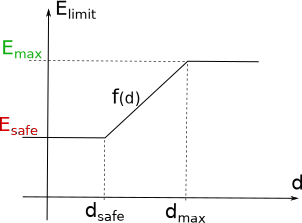
\includegraphics[width=0.5\columnwidth]{\figurepath/niveauEnergie_graph2}
    \caption{Evolution of the constraint on the kinetic energy of the robot in function of the distance $d$ between its end-effector and a considered obstacle.}
    \label{fig:niveauEnergie2}
\end{figure}
Based on the previous statements, three working zones, illustrated in Figure~\ref{fig:niveauEnergie1}, are distinguished for the dynamic behaviour of the robot when sharing its workspace with humans:
\begin{enumerate}
\item a safe zone for $d < d_{safe}$ in which the kinetic energy must be at most $E_{c_{safe}}$;
\item a working zone for $d_{safe} < d < d_{max}$ where the kinetic energy of the system is constrained as the human  moves towards the robot;
\item a third zone for $d > d_{max}$ in which maximum dynamic performances are allowed for the robot.
\end{enumerate}
\begin{figure}[h]
\centering
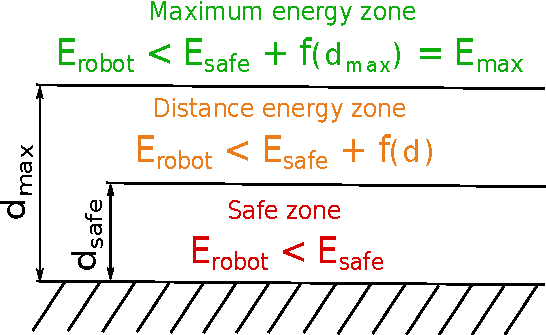
\includegraphics[width=0.5\columnwidth]{\figurepath/niveauEnergie_dessin}
\caption{Energy zones for the dynamic behaviour of the robot.} 
\label{fig:niveauEnergie1}
\end{figure}
When the relative distance between the approaching operator and the robot is decreasing, the system must be able to generate sufficient deceleration and jerk capabilities at the level of its end-effector\footnote{Or at the level of any potential collision point.} so it can properly react and cope with the imposed constraint on its kinetic energy. Two phases are distinguished when coping with such constraint in operational space: first, at the activation of the constraint, the amount of torque and jerk producible by the actuators of the robot and their corresponding dynamic capabilities in operational space must imperatively be considered to ensure that the system is capable of modulating its kinetic energy to make it cope with $E_{c_{limit}}$. The second phase is when the kinetic energy of the robot is equal to the maximum allowed value $E_{c_{limit}}$ (the constraint is activated), the variation of the function $f(d)$ must imperatively account for the reaction capabilities (i.e., producible deceleration and jerk in operational space) of the robot and this at every time-step. 
\\
When reactively coping with the constraint on kinetic energy, from the Work-Energy theorem, the amount of work exerted on the robot is equal to the variation of its kinetic energy. Moreover, this work can be expressed as a product between the \textit{equivalent braking force $F_{eq}$} applied on the end-effector and the braking distance:
\begin{equation}
\begin{split}
W &= \Delta E_c 
\\
&= F_{eq} (d-d_{safe}) 
\\
&= E_{c_{limit}}(d) - E_{c_{limit}}(d_{safe}) 
\\
&= f(d) - f(d_{safe}).
\end{split}
\end{equation}
The term $f$ represents the maximum energy that can be dissipated during the braking phase as the robot decreases its kinetic energy. By choosing this function to be linear inside the distance energy working zone (see Figure~\ref{fig:niveauEnergie2}), it can be written:
\begin{equation}
f(d) = K (d - d_{safe}).
\label{eq:k_fd}
\end{equation}
The smaller the braking distance $(d-d_{safe})$, the higher must be the slope coefficient of the function $f(d)$. $K$ represents the equivalent braking force applied at the level of the end-effector of the robot in the opposite direction to the obstacle. It depends on the available braking torque $\boldsymbol{\tau}_{braking}$, jerk capabilities and the instantaneous Jacobian $J(\vect{q}_{|k})_{EE}$ of the end-effector along the direction of the considered obstacle: 
\begin{equation}
\boldsymbol{\tau}_{braking}  = J(\vect{q}_{|k})_{EE}^{{EE,O}^T} K.
\end{equation}
For every time-step, the instantaneous equivalent braking force in Cartesian space at the level of the end-effector can be computed:
\begin{equation}
\argmax \limits_{K} \left\|K\right\|^{2},
\raisetag{-.5em} \\
\label{eq:K_maximizing_opt}
\end{equation}
s.t: 
%\begin{subequations}
%\label{eq:st_eqs}
%\begin{empheq}[left={}\empheqlbrace]{align}
%\boldsymbol{\tau}_{braking}  = J(\vect{q})_{EE}^{{EE,O}^T} K, \label{eq:st_eqs1} \\
%\vect{\tau}_{M} \leq \boldsymbol{\tau}_{breaking} \leq \vect{\tau}_{m} \label{eq:st_eqs2} 
%\end{empheq}
%\end{subequations}
\begin{subequations}
\begin{empheq}[left={}\empheqlbrace]{align}
&\boldsymbol{\tau}_{braking}  = J(\vect{q}_{|k})_{EE}^{{EE,O}^T} K, \\
&\vect{\tau}_{m} \leq \boldsymbol{\tau}_{braking} \leq \vect{\tau}_{M}, 
\end{empheq}
\end{subequations}
%$\boldsymbol{\tau}_{braking}  = J(\vect{q})_{EE}^{{EE,O}^T} K$ and $\vect{\tau}_{M} \leq \boldsymbol{\tau}_{breaking} \leq \vect{\tau}_{m}$
\\
with $\vect{\tau}_{braking}$ and $K$ the optimization variables. $\vect{\tau}_{M}$, $\vect{\tau}_{m}$ are the maximum and minimum torques producible by the actuators of the robot.
\\
For (\ref{eq:k_fd}), $K$ must be guaranteed over all the braking distance $d$. However, $\boldsymbol{\tau}_{braking}$ and $J(\vect{q}_{|k})_{EE}^{EE,O}$ can only be considered constant locally; the computation of $K$ depends then on the future configurations of the robot along the braking distance $d$. Given the non linear nature of robotic manipulators, predicting the evolution of $K$ is a complex problem. In the worst case, its value is very close to $0$\footnote{Especially near singularity configurations.} and to ensure safety, $E_{c_{limit}}$  should always be equal to $E_{c_{safe}}$, strongly limiting the dynamic performances of the robot. On the other hand, using actuators capable of deploying high braking torques/jerks allows to significantly decrease the braking distance $d$. In such case, a local estimation of $\boldsymbol{\tau}_{braking}$ and $J(\vect{q}_{|k})_{EE}^{EE,O}$ can be a good approximation. Given the global objectives of this work, an average value of $K$ ($>0$) is considered all over the workspace of the robot. 
%%%%%%%%%%%%%%%%%%%%%%%%%%SUBSUBSECTION%%%%%%%%%%%%%%%%%%%%%%%%%%%%%
%%%%%%%%%%%%%%%%%%%%%%%%%%SUBSUBSECTION%%%%%%%%%%%%%%%%%%%%%%%%%%%%%
\subsubsection{Pre-collision safety criterion extension}
The safety criterion previously introduced considers the squared relative velocity between the end-effector of the robot and a nearby obstacle. Therefore, there is no differentiation between the case where the robot is going towards the obstacle and when it is moving away from it. In a forbidden contact situation ($E_{c_{safe}} = 0$), $v = 0$ is imposed which forbids the robot from going towards the obstacle but also from moving away from it. To avoid constraining the motion of the robot in the opposite direction to the obstacle, the safety indicator $S_c$ during the \textit{free} movements of the robot can be signed:
\begin{equation}
S_c = \frac{1}{2} \hspace{0.5mm} \textnormal{sign(} v \textnormal{)} \hspace{0.5mm} m(\vect{q}_{|k})^{eq} v^2,
\label{eq:S_2}
\end{equation}
with $\textnormal{sign}(v) = 1$ when the end-effector  is getting closer to the considered obstacle. 
\\
The safety criterion can finally be written: 
\begin{equation}
S_c \leq E_{c_{safe}} +  K (d - d_{safe}),
\end{equation}
with $S_c$ defined by (\ref{eq:S_2}). \\
As previously explained in Subsection \ref{subsec:relEcEp}, an other approach to constrain the kinetic energy of the robot is to limit the amount of potential energy instantaneously \textit{injected} in its controller during  \textit{free} movements. Between two consecutive control time-steps, this potential energy changes the kinetic energy of the robot from $E_{c_{|k}}^{EE,O}$ to $E_{c_{|k+1}}^{EE,O}$:
\begin{equation}
E_{c_{|k+1}}^{EE,O} - E_{c_{|k}}^{EE,O} = E_{p_{|k}}^{EE,O} \Rightarrow E_{c_{|k}}^{EE,O} + E_{p_{|k}}^{EE,O} = E_{c_{|k+1}}^{EE,O} \leq E_{c_{limit}}
\label{eq:second_constr_on_Ec_0}
\end{equation}
Based on (\ref{eq:Ec_var_eq_Ep2}) and (\ref{eq:second_constr_on_Ec_0}), the constraint on kinetic energy can be written as a constraint on the potential energy \textit{injected} in the controller of the robot at each time-step: 
\begin{equation}
S_c = E_{c_{|k+1}}^{EE,O} = \underbrace{E_{c_{|k}}^{EE,O}}_{measured} + S_{p_{free}} \leq E_{c_{limit}} \Leftrightarrow S_{p_{free}} \leq \underbrace{E_{c_{safe}} +  K (d - d_{safe})}_{E_{c_{limit}}} - \underbrace{E_{c_{|k}}^{EE,O}}_{measured},
\label{eq:second_constr_on_Ec}
\end{equation}
with $S_{p_{free}}$ as in (\ref{eq:Sp_free_mvts}) the amount of potential energy instantaneously injected in the controller of the robot considering its movement towards a considered obstacle $O$. Using (\ref{eq:second_constr_on_Ec}), the kinetic energy of the robot is tracked then saturated when it reaches its maximum allowed limit by acting on the amount of potential energy $S_{p_{free}}$ injected in the controller of the robot. 
%%%%%%%%%%%%%%%%%%%%%%%%%%SUBSECTION%%%%%%%%%%%%%%%%%%%%%%%%%%%%%
%%%%%%%%%%%%%%%%%%%%%%%%%%%%%%%%%%%%%%%%%%%%%%%%%%%%%%%%%%%%%%%%%
%%%%%%%%%%%%%%%%%%%%%%%%%%SUBSECTION%%%%%%%%%%%%%%%%%%%%%%%%%%%%%
\subsection{Safety limit value for the physical-contact safety indicator}
For $S_{p_{contact}}$, the safety criterion represents the maximum amount $E_{p_{limit}}$ of potential energy allowed to be accumulated in the controller of the robot during physical contact with its environment. The value of $E_{p_{limit}}$ depends on several aspects: The desired degree of compliance of the robot during physical contact, the maximum allowed contact force and more importantly, the amount of kinetic energy this potential energy transforms into in case physical contact is released. Indeed, in such situation, the potential energy $E_{p_{limit}}$ accumulated in the controller of the robot is to be rapidly transformed into kinetic one and if any collision with a nearby operator occurs, the resulting impact force $F_{impact}$ may be harmful. Therefore, the maximum value acceptable for $E_{p_{limit}} = E_{p_{safe}}$ should never be superior to $E_{c_{safe}}$. The constraint on the potential energy generated between the robot and its environment during physical contact can be written: 
\begin{equation}
\begin{split}
S_{p_{contact}} \leq E_{p_{limit}} = E_{p_{safe}} \\
\textnormal{With: }
0 \leq E_{p_{safe}} \leq E_{c_{safe}}
\end{split}
\label{eq:Ep_constr_a}
\end{equation}
%\begin{figure}
%    \centering
%	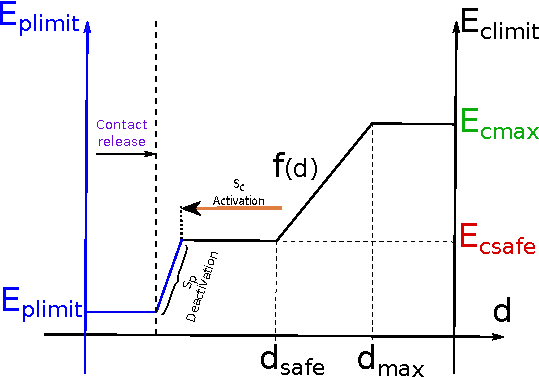
\includegraphics[width=0.7\columnwidth]{\figurepath/niveauEnergie_graph22}
%    \caption{Evolution of the kinetic energy constraint depending on the distance $d$ between the end-effector and the obstacle.}
%    \label{fig:niveauEnergie22}
%\end{figure}
\begin{figure}
    \centering
	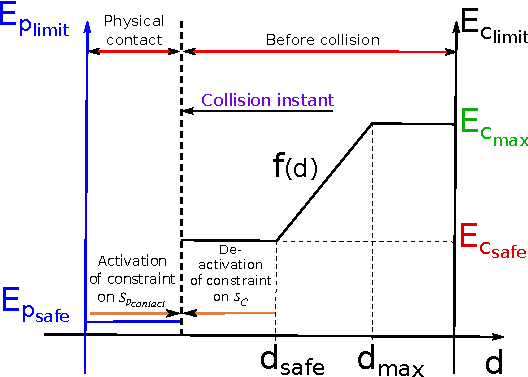
\includegraphics[width=0.8\columnwidth]{\figurepath/niveauEnergie_graph21}
    \caption{Evolution of the constraints on the kinetic and potential energies of the robot in function of the distance $d$ between its end-effector and the considered obstacle.}
    \label{fig:niveauEnergie21}
\end{figure}
%%%%%%%%%%%%%%%%%%%%%%%%%%SUBSECTION%%%%%%%%%%%%%%%%%%%%%%%%%%%%%
%%%%%%%%%%%%%%%%%%%%%%%%%%%%%%%%%%%%%%%%%%%%%%%%%%%%%%%%%%%%%%%%%
%%%%%%%%%%%%%%%%%%%%%%%%%%SUBSECTION%%%%%%%%%%%%%%%%%%%%%%%%%%%%%
\section{Energy constraints implementation}
\label{subsec:Econstr_acti_deacti}
Constraints on kinetic (\ref{eq:Ec_constr_a}) and potential (\ref{eq:Ep_constr_a}) energies can be implemented into an optimization control scheme and used to modulate the energy of a robotic manipulator during different interaction phases with its environment. Before physical contact and during the approach of the human operator, only the constraint on kinetic energy (\ref{eq:Ec_constr_a}) is needed. At collision, this constraint ensures that a safe amount of kinetic energy is dissipated creating a non hazardous impact force. At this stage, collision between the robot and its environment can be detected (using for example the proprioceptive articular torque sensors), and as it is no longer needed, the constraint on $S_c$ can be removed and replaced by the constraint on potential energy (\ref{eq:Ep_constr_a}) (see Fig.~\ref{fig:niveauEnergie21}). At the establishment of physical contact, potential energy within the human-robot system starts increasing to reach its maximum allowed value $E_{p_{limit}} = E_{p_{safe}}$. Depending on $E_{p_{safe}}$, the robot is more or less compliant and can be moved easily. When physical contact is released, the constraint on potential energy can be removed and the one on kinetic energy (\ref{eq:Ec_constr_a}) reintroduced in the configuration of the controller to prevent hazardous movements of the robot. 
%%%%%%%%%%%%%%%%%%%%%%%%%%SUBSECTION%%%%%%%%%%%%%%%%%%%%%%%%%%%%%
%%%%%%%%%%%%%%%%%%%%%%%%%%%%%%%%%%%%%%%%%%%%%%%%%%%%%%%%%%%%%%%%%
%%%%%%%%%%%%%%%%%%%%%%%%%%SUBSECTION%%%%%%%%%%%%%%%%%%%%%%%%%%%%%
\section{Task energy profile} 
\label{subsec:Task_energy_profile}
In case of a trajectory tracking task, the amount of potential energy $E_{p_{|k}}$ (\ref{eq:Ec_eq_sum_Ep_a}) instantaneously \textit{injected} in the  controller of the robot can be measured at every time-step. As soon as $E_{p_{|k}}$ is injected, the pulling force derived from it is created and drives the robot along its discretized trajectory. Because of this discretization, every time-step, only a small amount of potential energy $E_{p_{|k}}$ is injected and promptly transformed into kinetic one as the robot moves. For a repetitive trajectory tracking task, the energy profile $E_{p_{profile}}(t)$ (with $E_{p_{profile}}(t=k \delta t) = E_{p_{|k}}$) can be initially registered during the repetitive \textit{free} movements of the robot. Finally this profile can be used to limit the instantaneous amount of potential energy $E_{p_{|k}}$ the controller of the robot is allowed to contain at every time-step. Therefore, in case of a deliberate or accidental collision/contact, this constraint prevents the generation of large amounts of potential energy\footnote{The potential energy during physical contact is the extension of the potential energy \textit{injected} in the controller of the robot during its free movements.} and thus of hazardous contact forces between the robot and its environment. $E_{p_{profile}}(t)$ is then used as $E_{p_{safe}}$ during physical contact phases.
To resume:
\begin{itemize}
\item Every repetitive trajectory tracking task has its own energy profile. Namely, the minimum amount of energy needed to accomplish the assigned task.
\item This energy profile defined in operational space\footnote{Can also be defined in joint space.} is altered in case of any contact with the environment, more energy accumulates in the controller of the robot.
\item A constraint on the instantaneously allowed amount of potential energy in the controller prevents the robot from crushing any obstacle at the establishment of a physical contact. 
\end{itemize}
The constraint on the \textit{task energy profile} of a trajectory tracking task can be expressed at the level of any potential collision point $C$. It is written at the end-effector of the robot:   
\begin{equation}
%S_{p_{free}}\footnote{Note: $S_p$ was previously defined as the safety indicator during physical contact phases. However, as explained, potential energy exists in the system even during free movements of the robot. $S_p$ is finally used to quantify the generated potential energy for both the pre and post collision phases.} \leq E_{p_{limit}} = E_{p_{profile}} 
%S_{p_{profile}} = m(\vect{q}_{|k})_{EE,EE^*}^{eq} \ddot{X}_{EE_{|k}^{EE,EE^*} (\vect{X}_{EE_{|k}}^{*} - \vect{X}_{EE_{|k}}) \vect{n}_EE \leq E_{p_{limit}} = \underbrace{E_{p_{profile}}(t)}_{registred} 
S_{p_{profile}} = m(\vect{q}_{|k})_{EE,EE^*}^{eq} \ddot{X}_{EE_{|k}}^{EE,EE^*} \left(\vect{X}_{EE_{|k}}^{*} - \vect{X}_{EE_{|k}}\right) \vect{n}_{EE} \leq E_{p_{limit}}.
\label{eq:Ep_constr_30}
\end{equation} 
Note that the expression of $S_{p_{profile}}$ is the same as the expression of $S_{p_{contact}}$ that has been defined as the robot's safety indicator exclusively for the physical contact phase (\ref{eq:Ep_constr_221}). The safety indicator related to the controller's task energy profile $S_{p_{profile}}$ on the other hand, is defined for both the \textit{free movements} and the \textit{physical contact} phases.  
Constraining the task energy profile of the controller using (\ref{eq:Ep_constr_30}), prevents the robot from deploying any additional energy than what is needed at time-step $k$ for an optimal completion of its trajectory tracking task. As it is activated only in case of collisions/physical contact between the robot and its environment, this constraint can always be included in the controller and used as a low-level security layer without altering the tracking performances related to the assigned task. Even if collisions with the environment are not detected\footnote{For example in case of a fail of an exteroceptive sensor used to detect the collision.}, the robot will automatically comply to any external force preventing therefore the generation of harmful contact forces. \\
When the constraint on the task energy profile (\ref{eq:Ep_constr_30}) is used to limit the potential energy injected at each time-step in the system, (\ref{eq:second_constr_on_Ec}) or (\ref{eq:Ec_constr_first}) can simultaneously be implemented in the controller and used to limit the deployed kinetic energy. Both constraints ((\ref{eq:Ep_constr_30}) with (\ref{eq:second_constr_on_Ec})) or ((\ref{eq:Ep_constr_30}) with (\ref{eq:Ec_constr_first})) are compatible and can be implemented \textit{at the same time} in the optimization control scheme. \\
On the other hand, in case $E_{p_{limit}}$ is fixed $< E_{p_{profile}}$ in (\ref{eq:Ep_constr_30}), the performance of the trajectory tracking task will inevitably be deteriorated. Indeed, $E_{p_{profile}}$ is the minimum amount of potential energy the system needs to transform into kinetic one to accomplish its task in the most optimal way. At every time-step $k$, $E_{p_{profile}}$ can be written:
\begin{equation}
E_{p_{profile}}(t=k \delta t) = m(\vect{q}_{|k})_{EE,EE^*}^{eq} \ddot{X}_{EE_{|k}} \left(\vect{X}_{EE_{|k}}^{*} - \vect{X}_{EE_{|k}}\right) \vect{n}_{EE}. 
\label{eq:Ep_profile_computation}
\end{equation} 
Or when decoupled along the $\vect{x}$, $\vect{y}$ and $\vect{z}$ axis in operational space (the desired trajectory in Cartesian space being fed to the controller independently along these 3 axis): 
\begin{subequations}
\label{eq:Ep_profile_computation_3_axis}
\begin{empheq}[left={}\empheqlbrace]{align}
E_{p_{profile}}^{x} &= m(\vect{q}_{|k})_{x}^{eq} \ddot{X}_{EE_{|k}}^{\vect{x}} \left(\vect{X}_{x_{|k}}^{*} - \vect{X}_{x_{|k}}\right) \vect{x}, \label{eq:eqer} \\
E_{p_{profile}}^{y} &= m(\vect{q}_{|k})_{y}^{eq} \ddot{X}_{EE_{|k}}^{\vect{y}} \left(\vect{X}_{x_{|k}}^{*} - \vect{X}_{x_{|k}}\right) \vect{y}, \label{eq:eqet} \\
E_{p_{profile}}^{z} &= m(\vect{q}_{|k})_{z}^{eq} \ddot{X}_{EE_{|k}}^{\vect{z}} \left(\vect{X}_{x_{|k}}^{*} - \vect{X}_{x_{|k}}\right) \vect{z}. \label{eq:eqey} 
\end{empheq}
\end{subequations}
Which when saturated allows enabling compliance to physical contact independently along the desired axis.
%%%%%%%%%%%%%%%%%%%%%%%%%%%%%%%%%%%%%%%%%%%%%%%%%%%%%%%%%
                 %Safe dynamic controller%
%%%%%%%%%%%%%%%%%%%%%%%%%%%%%%%%%%%%%%%%%%%%%%%%%%%%%%%%%                         
\section{Safe dynamic controller}
\label{sec:safe_controller}
In this section a dynamic controller that can ensure safety for both the robot and its environment is proposed. The objective is to compute at every time-step the control torque $\boldsymbol{\tau}_{|k}^{c}$ in order to perform a trajectory tracking task while coping with a number of constraints: 
\begin{itemize}
\item satisfying the introduced safety criteria to prevent harmful collision and contact forces; 
\item coping with the limits corresponding to the articular physical capabilities of the robotic manipulator.
\end{itemize}
%%%%%%%%%%%%%%%%%%%%%%%%%%SUBSECTION%%%%%%%%%%%%%%%%%%%%%%%%%%%%%
%%%%%%%%%%%%%%%%%%%%%%%%%%%%%%%%%%%%%%%%%%%%%%%%%%%%%%%%%%%%%%%%%
%%%%%%%%%%%%%%%%%%%%%%%%%%SUBSECTION%%%%%%%%%%%%%%%%%%%%%%%%%%%%%
%\section{The QP form and articular constraints incompatibility cases}
%This section aims at establishing the general formulation of the constrained, redundant dynamic reactive control scheme. The objective is to compute the control torque $\boldsymbol{\tau}_{|k}^{c}$ in order to perform a trajectory tracking task in joint space while coping at every time-step with articular position, velocity, acceleration and jerk constraints. We highlight the fact that in this particular case the desired trajectories for the joint of the robot are \textit{discovered at every time-step} (tele-operation analogue situation) and are not known in advance. Incompatibility cases related to the classic way of expressing articular constraints are discussed. 
%\subsection{Task formulation}
%The objective function of the controller is defined as an error to be minimized. A joint-space acceleration controller is considered and the error is between the expected acceleration $\vect{\ddot{q}}^c$ and the real acceleration $\vect{\ddot{q}}$ of the robot's end-effector. It is written in function of the control input $\vect{\tau}_{|k}^{c}$:
%\begin{equation}
% \vect{\ddot{X}}^{c} = J(\vect{q}) M(\vect{q})^{-1} \left(\boldsymbol{\tau}_{|k}^{c} - \vect{b}(\vect{q},\vect{\dot{q}})\right) + \dot{J}(\vect{q}) \vect{\dot{q}}
%\label{Xddot}
%\end{equation}
%$\vect{b}(\vect{q},\vect{\dot{q}})$ are the non linear terms, namely gravity, Coriolis and centrifugal induced generalized forces. $M(\vect{q})$ is the joint space inertia matrix of the robot. $\vect{\ddot{X}}^c$ can be computed with a PD controller to track a desired trajectory (position $\vect{X}(t)^\star$ and velocity  $\vect{\dot{X}}(t)^\star$, \textit{discovered at every time-step}). The acceleration task function to be minimized is written:
%\hspace{-2mm}
%\begin{equation}
%\resizebox{.911\hsize}{!}{$\vect{g}\left(\boldsymbol{\tau}_{|k}^{c},\vect{\ddot{X}}^c\right) =  \vect{\ddot{X}}^c - \left(J(\vect{q}) M(\vect{q})^{-1} \left(\boldsymbol{\tau}_{|k}^{c} - \vect{b}(\vect{q},\vect{\dot{q}}) \right) + \dot{J}(\vect{q}) \vect{\dot{q}}\right)$}
%\label{accelerationError}
%\end{equation}
%\subsection{Controller formulation}
%The proposed control strategy computes the control torque by minimizing the norm of the  cartesian acceleration task function expressed in the following quadratic form: 
%\begin{equation}
%\argmin \limits_{\boldsymbol{\tau}_{|k}^{c}}  \left\| \vect{g}\left(\boldsymbol{\tau}_{|k}^{c},\vect{\ddot{X}}^c\right) \right\|_{Q_t}^2 + \epsilon  \| \boldsymbol{\tau}_{|k}^{c} \|_{Q_r}^2,
%\label{eq:ctrl_pb}
%\end{equation}
%%subject to (\ref{eq:qddot_FINAL_CONSTR_1}) and (\ref{eq:qddot_FINAL_CONSTR_2}).
%\\
%$Q_t$ and $Q_r$ are  positive semi-definite weighting matrices and $\| \vect{a} \|_{Q}$ is the $Q-$weighted euclidean norm of $a$. $\epsilon  \| \boldsymbol{\tau}_{|k}^{c} \|_{Q_r}^2$ with $\epsilon << 1$ serves as a regularization task in order to ensure the uniqueness of the control solution and to minimize the norm of the computed control torque. It can be shown that the quadratic forms composing the tasks can be written as functions of positive semidefinite matrices. This LQP optimization problem is therefore convex and admits a unique global solution. 
%$\vect{\ddot{q}}_{|k}^{c}$ and $\vect{\tau}_{|k}^{c}$ are the control optimization variables: 
%\begin{equation}
%M(\vect{q}) \vect{\ddot{q}}_{|k}^{c} + \vect{b}(\vect{q},\vect{\dot{q}}) = \vect{\tau}_{|k}^{c}
%\label{eq:dyn_eq}
%\end{equation}
%\\ 
%In addition to the equality constraints corresponding to the dynamic equation \eqref{eq:dyn_eq}, the problem is also subject to inequality constraints described in the upcoming sections. 

\subsection{Task formulation}
The objective function of the controller is defined as an error to be minimized. It could be for example an acceleration task if the
robot has to track a trajectory, or a wrench task if the interaction wrench with the environment needs to be controlled. In the presented work, a trajectory tracking performance is considered. A Cartesian acceleration task is defined as an error between the desired acceleration $\vect{\ddot{X}}^{*}$ and the expected acceleration $\vect{\ddot{X}}^{c}$ of the end-effector of the robot. Considering $\vect{\ddot{X}}^{c} =  J(\vect{q}_{|k})_{EE} \vect{\ddot{q}}_{|k}^{c} + \dot{J}(\vect{q}_{|k})_{EE} \vect{\dot{q}}_{|k}$, with $J(\vect{q}_{|k})_{EE}$ the instantaneous Jacobian related to the end-effector, using the equation of motion of the system, $\vect{\ddot{X}}^{c}$ can also be written as function of the control input $\vect{\tau}_{|k}^{c}$:
\begin{equation}
\vect{\ddot{X}}^{c} = J(\vect{q}_{|k}) M(\vect{q}_{|k})^{-1} \left(\vect{\tau}_{|k}^{c} - \vect{b}(\vect{q}_{|k},\vect{\dot{q}}_{|k})\right) + \dot{J}(\vect{q}_{|k}) \vect{\dot{q}}_{|k},
\label{Xddot}
\end{equation}
$\vect{b}(\vect{q}_{|k},\vect{\dot{q}}_{|k})$ are the non linear terms of the equation of motion, namely gravity, Coriolis and centrifugal induced generalized forces. $\vect{\ddot{X}}^{*}$ can be computed with a PD controller and a feed-forward acceleration term $\vect{\ddot{X}}_{ff}$ in order to track a desired position $\vect{X}^*$ and velocity $\vect{\dot{X}}^*$ in operational space:
\begin{equation}
\vect{\ddot{X}}^{*} = \vect{\ddot{X}}_{ff} + K_p\left(\vect{X}^{*}-\vect{X}\right) + K_d\left(\vect{\dot{X}}^{*}-\vect{\dot{X}}\right),
\label{accelerationError}
\end{equation}
where $K_p$, $K_d$ $\in \mathbb{R}^{+}$ are the proportional and derivative gains. \\
The acceleration task function to be minimized is finally written:
\begin{equation}
\vect{g}\left(\vect{\tau}_{|k}^c,\vect{\ddot{X}}^c\right) =  \vect{\ddot{X}}^* - \left(J(\vect{q}_{|k}) M(\vect{q}_{|k})^{-1} \left(\vect{\tau}_{|k}^{c} - \vect{b}(\vect{q}_{|k},\vect{\dot{q}}_{|k}) \right) + \dot{J}(\vect{q}_{|k}) \vect{\dot{q}}_{|k}\right).
\label{accelerationError}
\end{equation}
%%
%\subsection{Task formulation}
%The objective function of the controller is defined as an error function to be minimized. It could be for example an acceleration task if the
%robot has to perform a trajectory tracking, or a wrench task if the wrench applied on the environment has to be controlled.
%\\
%In this work, a trajectory tracking performance is considered. A cartesian acceleration task is then defined as an error between the expected acceleration $\vect{\ddot{X}}^c$ and the real acceleration $\vect{\ddot{X}}$ of the robot-end effector. Considering $\vect{\ddot{X}} =  J(\vect{q}) \vect{\ddot{q}} + \dot{J}(\vect{q}) \vect{\dot{q}}$ (where $J(\vect{q})$ is the Jacobian of the end-effector), it can be written as function of the control input using the equation of motion of the system:
%\begin{equation}
% \vect{\ddot{X}} = J(\vect{q}) M(\vect{q})^{-1} \left(\boldsymbol{\tau} - \vect{b}(\vect{q},\vect{\dot{q}})\right) + \dot{J}(\vect{q}) \vect{\dot{q}},
%\label{Xddot}
%\end{equation}
%where $\vect{b}(\vect{q},\vect{\dot{q}})$ are the non linear terms of the equation of motion, namely gravity, Coriolis and centrifugal induced generalized forces. $\vect{\ddot{X}}^c$ can be computed with a PD controller with feed-forward term in order to track some desired trajectory $\vect{X}(t)^\star$. The acceleration task function to minimize can then be written:
%\begin{equation}
% \vect{g}\left(\boldsymbol{\tau},\vect{\ddot{X}}^c\right) =  \vect{\ddot{X}}^c - \left(J(\vect{q}) M(\vect{q})^{-1} \left(\boldsymbol{\tau} - \vect{b}(\vect{q},\vect{\dot{q}}) \right) + \dot{J}(\vect{q}) \vect{\dot{q}}\right) .
%\label{accelerationError}
%\end{equation}
%%%%%%%%%%%%%%%%%%%%%%%%%%SUBSECTION%%%%%%%%%%%%%%%%%%%%%%%%%%%%%
%%%%%%%%%%%%%%%%%%%%%%%%%%%%%%%%%%%%%%%%%%%%%%%%%%%%%%%%%%%%%%%%%
%%%%%%%%%%%%%%%%%%%%%%%%%%SUBSECTION%%%%%%%%%%%%%%%%%%%%%%%%%%%%%
\subsection{Constraints formulation}
\subsubsection{Articular constraints}
First, the limitations corresponding to the articular physical capabilities of the robot must be accounted for when solving the control problem. The computed control input $\boldsymbol{\tau}_{|k}^{c}$ at time-step $k$ must be such that the considered limits are never violated and the \textit{viability} of the state of the robot preserved. The actuators limitations are considered at the following levels: $\vect{q}$, $\vect{\dot{q}}$, $\vect{\ddot{q}}$ and $\vect{\dddot{q}}$. Usually, the constraints corresponding to the actuation limitations are expressed as inequalities and activated only one time-step before reaching their respective Max/mi boundaries. As explained in Chapter~\ref{chap:Constrcomp}, this can result into \textit{incompatibility problems} that may render the control problem impossible solve. For e.g., no sufficient articular torque/jerk may be producible to cope with an articular position or velocity limit within only one control time-step $=~1ms$. Therefore, it is the new formulations of the constraints introduced in Chapter~\ref{chap:Constrcomp} that are hereby used to bound the physical capabilities of the actuators of the robot. The inequality constraints corresponding to the articular physical limitations of the robot are written:
\begin{subequations}
\label{eq:const_1_literature23}
\begin{empheq}[left={}\empheqlbrace]{align}
\vect{q}_{|k+n_{15}+n_{17}+n_{19}} \leq \vect{q}_{M},\label{eq:cnt_lit_11}\\
\vect{q}_{|k+n_{16}+n_{18}+n_{20}} \geq \vect{q}_{m},\label{eq:cnt_lit_11_bis}\\
\vect{\dot{q}}_{|k+n_1} \leq \vect{\dot{q}}_{M},\label{eq:cnt_lit_22}\\  
\vect{\dot{q}}_{|k+n_2} \geq \vect{\dot{q}}_{m},\label{eq:cnt_lit_22_bis}\\    
\boldsymbol{\tau}_{m}   \leq \boldsymbol{\tau}_{|k}^{c}\hspace{4mm}\leq \boldsymbol{\tau}_{M},\label{eq:cnt_lit_44}\\
\vect{\dddot{q}}_{m}  \leq \vect{\dddot{q}}_{|k+1}\leq \vect{\dddot{q}}_{M},\label{eq:cnt_lit_55}
\end{empheq}
\end{subequations}
\\
with $\vect{q}_{|k+n_{15}+n_{17}+n_{19}}$, $\vect{q}_{|k+n_{16}+n_{18}+n_{20}}$ as in (\ref{eq:q_evolution_with_const_qdddot_m_const_qddot_m_const_qdddot_M}) and $\vect{\dot{q}}_{|k+n_1}$, $\vect{\dot{q}}_{|k+n_2}$ equivalent to (\ref{eq:q_dot_evolution_with_const_qdddot_m}) from Chapter~\ref{chap:Constrcomp}. To be easily accounted for, these constraints must be expressed as a function of the control variable $\vect{\ddot{q}}_{|k}^{c}$. Given the state of the system at instant $k$ and a discrete linear approximation of the behaviour of the robot in joint space:  
\begin{subequations}
\begin{empheq}[left={}\empheqlbrace]{align}
\textit{f}_{\chi}(\vect{q}_m, \vect{\dddot{q}}_M, \vect{\ddot{q}}_M, \vect{\dddot{q}}_m, n_{16}, n_{18}, n_{20}) \leq  &\vect{\ddot{q}}_{|k}^{c} \leq \textit{f}_{\phi}(\vect{q}_M, \vect{\dddot{q}}_m, \vect{\ddot{q}}_m, \vect{\dddot{q}}_M, n_{15}, n_{17}, n_{19}), \label{eq:cnt_lit_111}\\
\textit{f}_{\beta}(\vect{\dot{q}}_{|k}, \vect{\dot{q}}_m, \vect{\dddot{q}}_M, n_2) \leq  &\vect{\ddot{q}}_{|k}^{c} \leq \textit{f}_{\alpha}(\vect{\dot{q}}_{|k}, \vect{\dot{q}}_M, \vect{\dddot{q}}_m, n_1), \label{eq:cnt_lit_222}\\
\boldsymbol{\tau}_{m} \leq  &\boldsymbol{\tau}_{|k}^{c} \leq \boldsymbol{\tau}_{M}, \label{eq:cnt_lit_333}\\
\vect{\dddot{q}}_{m} \delta t+\vect{\ddot{q}}_{|k} \leq  &\vect{\ddot{q}}_{|k}^{c} \leq \vect{\dddot{q}}_{M} \delta t+\vect{\ddot{q}}_{|k}, \label{eq:cnt_lit_444}
\end{empheq}
\label{eq:const_1_literature1}
\end{subequations}
\\
with $\textit{f}_{\chi}$, $\textit{f}_{\phi}$, $\textit{f}_{\beta}$ and $\textit{f}_{\alpha}$ respectively equivalent to (\ref{eq:q_ddot_posi_acc_jerk_comp_complete_1}), (\ref{eq:q_ddot_posi_acc_jerk_comp_complete_2}), (\ref{eq:q_ddot_vel_jerk_comp_aa_n1}) and (\ref{eq:q_ddot_vel_jerk_comp_aa_n2}) from Chapter~\ref{chap:Constrcomp}. \\
Finally, in addition to the articular inequality constraints, the system is also subject to linear equality constraints corresponding to its dynamic model:
\begin{equation}
M(\vect{q}_{|k}) \vect{\ddot{q}}_{|k}^{c} + \vect{b}(\vect{q}_{|k},\vect{\dot{q}}_{|k}) = \vect{\tau}_{|k}^{c}
\label{eq:dyn_eq_aab}
\end{equation}
%%%%%%%%%%%%%%%%%%%%%%%%%%%%%%%%%%%%%%%%%%%%%%%%%%%%%%%%%%%%%%%%%
\subsubsection{Energy related constraints}
In an equivalent way, the introduced safety indicators $S_{c}$, $S_{p_{free}}$, $S_{p_{contact}}$ and $S_{p_{profile}}$ can be expressed as functions of the dynamic control variable $\vect{\ddot{q}}_{|k}^{c}$. \\
First, based on (\ref{eq:Ec_constr_a}), during the \textit{free} movements of the robot, $S_c$ can be written:
\begin{equation} 
S_{c} = E_{c_{|k+1}}^{EE,O} = \frac{1}{2} \textnormal{sign}\left(v_{EE_{|k+1}}^{EE,O}\right) m(\vect{q}_{|k})_{EE,O}^{eq} v_{EE_{|k+1}}^{{EE,O}^2},
\label{eq:eq1}
\end{equation}
With: 
\begin{subequations}
\label{eq:const_eqs}
\begin{empheq}[left={}\empheqlbrace]{align}
v_{EE_{|k+1}}^{EE,O} &=  J(\vect{q}_{|k})_{EE}^{EE,O} \vect{\dot{q}}_{|k+1}, \label{eq:eq3} \\
\vect{\dot{q}}_{|k+1} \hspace{3.6mm} &= \vect{\dot{q}}_{|k} + \vect{\ddot{q}}_{|k}^{c} \delta t. \label{eq:eq4} 
\end{empheq}
\end{subequations}
Considering the \textit{second formulation} (\ref{eq:second_constr_on_Ec}) of the same kinetic energy based safety indicator $S_{c}$, it can also be written: 
\begin{equation} 
S_{c} = E_{c_{|k+1}}^{EE,O} = \underbrace{E_{c_{|k}}^{EE,O}}_{measured} + S_{p_{free}}\footnote{Here, $S_{p_{free}}$ is the injected \textit{potential energy} expressed at the level of the end-effector of the robot in the direction of the considered obstacle \textit{O} during the \textit{free} movements of the robot.} = E_{c_{|k}}^{EE,O} + m(\vect{q}_{|k})_{EE,O}^{eq} \ddot{X}_{EE_{|k}}^{EE,O} \left(\vect{X}_{EE_{|k+1}} - \vect{X}_{EE_{|k}}\right) \vect{n}_O,
\label{eq:eq2}
\end{equation}
\begin{equation} 
\textnormal{with: } 
\ddot{X}_{EE_{|k}}^{EE,O} = \dot{J}(\vect{q}_{|k})_{EE}^{EE,O} \vect{\dot{q}}_{|k} + J(\vect{q}_{|k})_{EE}^{EE,O} \vect{\ddot{q}}_{|k}^{c}.
\label{eq:v_futur}
\end{equation}
$X_{EE_{|k+1}}$ is the future position of the end-effector that can be estimated as:
\begin{equation}
\vect{X}_{EE_{|k+1}} = \underbrace{\vect{X}_{EE_{|k}}}_{measured} + \underbrace{\vect{\dot{X}}_{EE_{|k}}}_{measured} \delta t + \frac{1}{2} \underbrace{\vect{\ddot{X}}_{EE_{|k}}}_{measured} \delta t^2.
\label{eq:X_k1_estimated}
\end{equation}
On the other hand, during physical contact, $S_{p_{contact}}$ is expressed: 
\begin{equation} 
S_{p_{contact}} =  m(\vect{q}_{|k})_{EE,*}^{eq} \ddot{X}_{EE_{|k}}^{EE,*} \left(\vect{X}_{EE_{|k}}^{*} - \vect{X}_{EE_{|k}}\right) \vect{n}_{EE}, \\
\label{eq:Sp_phy_cont_expre}
\end{equation}
\begin{equation} 
\textnormal{with: } 
\ddot{X}_{EE_{|k}}^{EE,*} = \dot{J}(\vect{q}_{|k})_{EE}^{EE,*} \vect{\dot{q}}_{|k} + J(\vect{q}_{|k})_{EE}^{EE,*} \vect{\ddot{q}}_{|k}^{c} .
\label{eq:Sp_phy_cont_expre_with}
\end{equation} 
Or independently along the $\vect{x}$, $\vect{y}$ and $\vect{z}$ axis in Cartesian space, $S_{p_{contact}}$ can be decomposed: 
\begin{subequations}
\label{eq:Ep_constr_2_3_axis}
\begin{empheq}[left={}\empheqlbrace]{align}
S_{p_{contact}}^{x} &= m(\vect{q}_{|k})_{x}^{eq} \ddot{X}_{EE_{|k}}^{\vect{x}} \left(\vect{X}_{x_{|k}}^{*} - \vect{X}_{x_{|k}}\right) \vect{x}, \label{eq:eqer} \\
S_{p_{contact}}^{y} &= m(\vect{q}_{|k})_{y}^{eq} \ddot{X}_{EE_{|k}}^{\vect{y}} \left(\vect{X}_{y_{|k}}^{*} - \vect{X}_{y_{|k}}\right) \vect{y}, \label{eq:eqet} \\
S_{p_{contact}}^{z} &= m(\vect{q}_{|k})_{z}^{eq} \ddot{X}_{EE_{|k}}^{\vect{z}} \left(\vect{X}_{z_{|k}}^{*} - \vect{X}_{z_{|k}}\right) \vect{z}. \label{eq:eqey} 
\end{empheq}
\end{subequations}
Finally, the constraints related to $S_c$ and $S_p$ that will be tested in simulation then on the real robot using the proposed controller are as follows:
\begin{itemize}
\item \textbf{During the \textit{pre-collision} phase}: 
\begin{enumerate}
\item The constraint on the kinetic energy of the robot (first formulation):
\begin{equation} 
S_c =  \frac{1}{2} \textnormal{sign}\left(v_{EE_{|k+1}}^{EE,O}\right) m(\vect{q}_{|k})_{EE,O}^{eq} v_{EE_{|k+1}}^{{EE,O}^2} \leq E_{c_{limit}} = E_{c_{safe}} +  K (d - d_{safe}),
\label{eq:Safe_constr_1}
\end{equation}
with $\textnormal{sign}\left(v_{EE_{|k+1}}^{EE,O}\right)$ estimated by:
\begin{equation} 
\textnormal{sign}\left(v_{EE_{|k+1}}^{EE,O}\right) = \textnormal{sign}\left(v_{EE_{|k}}^{EE,O}+\underbrace{\ddot{X}_{EE_{|k}}^{EE,O}}_{measured} \delta t\right). 
\label{eq:sign_estimation}
\end{equation}
We recall that $\textnormal{sign}\left(v_{EE_{|k+1}}^{EE,O}\right)$ is positive for the movements of the robot towards the considered obstacle and negative otherwise.
\item The constraint on the kinetic energy of the robot (second formulation): 
\begin{equation} 
S_c =  E_{c_{|k}}^{EE,O} + S_{p_{free}} \leq E_{c_{limit}} = E_{c_{safe}} +  K (d - d_{safe}).
\label{eq:Safe_constr_2}
\end{equation}
Which transforms into: 
\begin{equation} 
%- m(\vect{q})_{EE,O}^{eq} \vect{\ddot{X}}_{EE_{|k}}^{EE,O} \left\| \vect{X}_{EE_{|k}} - \vect{X}_{EE_{|k+1}}\right\|_{EE,O} \leq E_{c_{limit}} - \underbrace{E_{c_{|k}}^{EE,O}}_{\textnormal{measured}} \hspace{4mm}\underbrace{-\epsilon_{d} \dot{E}_{c_{|k}}^{EE,O}}_{\textnormal{for regulation}} 
\underbrace{m(\vect{q}_{|k})_{EE,O}^{eq} \ddot{X}_{EE_{|k}}^{EE,O}  \left(\vect{X}_{EE_{|k+1} - \vect{X}_{EE_{|k}}}\right) \vect{n}_O}_{S_{p_{free}}} \leq E_{c_{limit}} - \underbrace{E_{c_{|k}}^{EE,O}}_{\textnormal{measured}},
\label{eq:Safe_constr_2_bis}
\end{equation}        
with $\vect{X}_{EE_{|k+1}}$ and $\ddot{X}_{EE_{|k}}^{EE,O}$ respectively as in (\ref{eq:X_k1_estimated}) and (\ref{eq:v_futur}). 
\end{enumerate}
\item \textbf{During the \textit{physical-contact} phase}: 
\begin{equation} 
S_{p_{contact}} = m(\vect{q}_{|k})_{EE, EE^*}^{eq} \ddot{X}_{EE_{|k}}^{EE, EE^*} \left(\vect{X}_{EE_{|k}}^{*} - \vect{X}_{EE_{|k}}\right) \vect{n}_{EE} \leq E_{p_{limit}} = E_{p_{safe}}.
\label{eq:Safe_constr_4}
\end{equation}
When decoupled along the $\vect{x}$, $\vect{y}$ and $\vect{z}$ axis in Cartesian space: 
\begin{subequations}
\label{eq:Safe_constr_4_3_axisaaa}
\begin{empheq}[left={}\empheqlbrace]{align}
S_{p_{contact}}^{x} &= m(\vect{q}_{|k})_{x}^{eq} \ddot{X}_{EE_{|k}}^{\vect{x}} \left(\vect{X}_{x_{|k}}^{*} - \vect{X}_{x_{|k}}\right) \vect{x} \leq E_{p_{safe}}^{x}, \label{eq:Safe_constr_4_x_axis} \\
S_{p_{contact}}^{y} &= m(\vect{q}_{|k})_{y}^{eq} \ddot{X}_{EE_{|k}}^{\vect{y}} \left(\vect{X}_{y_{|k}}^{*} - \vect{X}_{y_{|k}}\right) \vect{y} \leq E_{p_{safe}}^{y}, \label{eq:Safe_constr_4_y_axis} \\
S_{p_{contact}}^{z} &= m(\vect{q}_{|k})_{z}^{eq} \ddot{X}_{EE_{|k}}^{\vect{z}} \left(\vect{X}_{z_{|k}}^{*} - \vect{X}_{z_{|k}}\right) \vect{z} \leq E_{p_{safe}}^{z} \label{eq:Safe_constr_4_z_axis} 
\end{empheq}
\end{subequations}
Note: as formulated, constraints in (\ref{eq:Safe_constr_4}) and (\ref{eq:Safe_constr_4_3_axisaaa}) prevent the robot from generating harmful contact forces but only along the positive direction of the considered axis. With such formulations, contact forces are saturated during physical contact but as nothing prevents the accumulation of \textit{negative} \textit{potential energy} in the controller of the robot during physical contact, the robot cannot be pushed in the opposite direction. Which makes it dangerous regarding the expected \textit{safe} human-robot interaction. To enable the robot to be pushed along all the directions in operational space, it is the absolute value of its \textit{potential energy} that should be constrained. It is then saturated in both the positive and negative directions of the considered axis. (\ref{eq:Safe_constr_4}) and (\ref{eq:Safe_constr_4_3_axisaaa}) are thus rewritten: 
%\begin{equations}
%|S_{p_{contact}}| \leq E_{p_{safe}}\Leftrightarrow \begin{empheq}[left={}\empheqlbrace]{align}
%S_{p_{contact}} \leq  E_{p_{safe}}, \\
%S_{p_{contact}} \geq - E_{p_{safe}}. 
%\end{empheq}
%\label{eq:Safe_constr_41243negfinauul}
%\end{equations}
%\begin{equation} 
%\begin{split}
%\textit{S}_{|k+1}&\left\{\begin{array}{lcl}
%\vect{\dot{q}}_{|k+1} \hspace{1mm}= \vect{\dot{q}}_{|k} + \vect{\ddot{q}}_{|k} \delta t, \\
%\vect{\ddot{q}}_{|k+1} \hspace{1mm}= \vect{\ddot{q}}_{|k} + \vect{\dddot{q}}_{m} \delta t.
%\end{array}\right.\\
%\end{split}
%\label{eq:discretized_dynamics_vel}
%\end{equation}
\begin{subequations}
\label{eq:Safe_constr_4_3_axis12}
\begin{empheq}[left={|S_{p_{contact}}| \leq  E_{p_{safe}}\Leftrightarrow}\empheqlbrace]{align}
S_{p_{contact}} &\leq \hspace{2.9mm} E_{p_{safe}}, \label{eq:Safe_constr_4_x_axis_pos12}\\ 
S_{p_{contact}} &\geq - E_{p_{safe}}. \label{eq:Safe_constr_4_x_axis_neg12}
\end{empheq}
\end{subequations}
And when decoupled:
\begin{subequations}
\label{eq:Safe_constr_4_3_axis54}
\begin{empheq}[left={}\empheqlbrace]{align}
S_{p_{contact}}^{x} &\leq \hspace{2.9mm} E_{p_{safe}}^{x}, \label{eq:Safe_constr_4_x_axis_pos54} \\
S_{p_{contact}}^{x} &\geq -E_{p_{safe}}^{x}, \label{eq:Safe_constr_4_x_axis_neg54} \\
S_{p_{contact}}^{y} &\leq \hspace{2.9mm} E_{p_{safe}}^{y}, \label{eq:Safe_constr_4_y_axis_pos54} \\
S_{p_{contact}}^{y} &\geq -E_{p_{safe}}^{y}, \label{eq:Safe_constr_4_y_axis_neg54} \\
S_{p_{contact}}^{z} &\leq \hspace{2.9mm} E_{p_{safe}}^{z}, \label{eq:Safe_constr_4_z_axis_pos54} \\
S_{p_{contact}}^{z} &\geq -E_{p_{safe}}^{z}. \label{eq:Safe_constr_4_z_axis_neg54} 
\end{empheq}
\end{subequations}
\item \textbf{During both the \textit{pre-collision} and the \textit{physical-contact} phases}: \\
The constraint on the \textit{task energy profile} of the robot can be written:
\begin{equation} 
\left|S_{p_{profile}}\right| = \left|m(\vect{q})_{EE,*}^{eq} \ddot{X}_{EE_{|k}}^{EE,*} \left(\vect{X}_{EE_{|k}}^{*} - \vect{X}_{EE_{|k}}\right) \vect{n}_{EE} \right|\leq E_{p_{profile}}\footnote{Measured during the \textit{free} unconstrained movements of the robot.}+ \epsilon_{E_p}.
\label{eq:Safe_constr_3}
\end{equation}
Which can also be decoupled along the $\vect{x}$, $\vect{y}$ and $\vect{z}$ axis in Cartesian space:
\begin{subequations}
\label{eq:Safe_constr_3_axis}
\begin{empheq}[left={}\empheqlbrace]{align}
\left|S_{p_{profile}}^{x}\right| &= \left|m(\vect{q}_{|k})_{x}^{eq} \ddot{X}_{EE_{|k}}^{\vect{x}} \left(\vect{X}_{x_{|k}}^{*} - \vect{X}_{x_{|k}}\right) \vect{x} \right|\leq E_{p_{profile}}^{x} + \epsilon_{E_p}^{x}, \label{eq:eqAA} \\
\left|S_{p_{profile}}^{y}\right| &= \left|m(\vect{q}_{|k})_{y}^{eq} \ddot{X}_{EE_{|k}}^{\vect{y}} \left(\vect{X}_{y_{|k}}^{*} - \vect{X}_{y_{|k}}\right) \vect{y} \right|\leq E_{p_{profile}}^{y} + \epsilon_{E_p}^{y}, \label{eq:eqBB} \\
\left|S_{p_{profile}}^{z}\right| &= \left|m(\vect{q}_{|k})_{z}^{eq} \ddot{X}_{EE_{|k}}^{\vect{z}} \left(\vect{X}_{z_{|k}}^{*} - \vect{X}_{z_{|k}}\right) \vect{z} \right|\leq E_{p_{profile}}^{z} + \epsilon_{E_p}^{z}. \label{eq:eqCC}
\end{empheq}
\end{subequations}
The \textit{task energy profile} related constraints (\ref{eq:Safe_constr_3}) or (\ref{eq:Safe_constr_3_axis}) can be implemented simultaneously with the constraints on the kinetic energy of the robot: (\ref{eq:Safe_constr_1}) or (\ref{eq:Safe_constr_2}). A \textit{task energy profile} related constraint is defined for both the \textit{pre-collision} and \textit{physical-contact} interaction phases. It can therefore replace the constraint on the robot's \textit{potential energy} (\ref{eq:Safe_constr_4_3_axis54}) to render the robot more compliant when physical contact is established. $\epsilon_{E_p}$, $\epsilon_{E_p}^{x}$, $\epsilon_{E_p}^{y}$ and $\epsilon_{E_p}^{z}$ are constants used to compensate the repeatability related variations when registering the energy profiles: $E_{p_{profile}}(t)$, $E_{p_{profile}}^{x}(t)$, $E_{p_{profile}}^{y}(t)$ and $E_{p_{profile}}^{z}(t)$.
\end{itemize}
%%%%%%%%%%%%%%%%%%%%%%%%%%SUBSECTION%%%%%%%%%%%%%%%%%%%%%%%%%%%%%
%%%%%%%%%%%%%%%%%%%%%%%%%%%%%%%%%%%%%%%%%%%%%%%%%%%%%%%%%%%%%%%%%
%%%%%%%%%%%%%%%%%%%%%%%%%%SUBSECTION%%%%%%%%%%%%%%%%%%%%%%%%%%%%%
\subsection{Controller formulation}
\label{subsec:cntrl_frmulation}
The proposed controller computes the command torque by minimizing the norm of the  Cartesian acceleration task function expressed in the following quadratic form: 
\begin{equation}
\argmin \limits_{\boldsymbol{\tau}_{|k}^{c}, \vect{\ddot{q}}_{|k}^{c}}  \left\| \vect{g}\left(\boldsymbol{\tau}_{|k}^{c},\vect{\ddot{X}}^c\right) \right\|_{Q_t}^2 + \epsilon  \| \boldsymbol{\tau}_{|k}^{c} \|_{Q_r}^2,
\label{eq:ctrl_pbb}
\end{equation}
subject to the constraints regarding the physical articular capabilities of the robot (\ref{eq:const_1_literature1}) and to the equality constraints related to its dynamic model (\ref{eq:dyn_eq_aab}). The controller will also be tested with: 1) the first (\ref{eq:Safe_constr_1}) and second (\ref{eq:Safe_constr_2}) formulations of the constraint on the kinetic energy of the robot, 2) the constraint on the \textit{potential energy} that accumulates in its controller during physical contact (\ref{eq:Safe_constr_4}) and, 3) the constraint related to the \textit{task energy profile} (\ref{eq:Safe_constr_3}). \\
%Note: Because of possible incompatibility issues with the energy based constraints\footnote{Incompatibilities may arise from the amount of jerk needed to cope with an energy based constraint. If this amount is superior to the articular capabilities of the system, the LQP becomes unsolvable.}, the \textit{hard-codded} constraint on jerk (\ref{eq:cnt_lit_444}) will be removed from the controller when any energy related constraint is to be activated.
Note: because of possible incompatibility issues that may occur between the \textit{energy based constraints} and the constraint on articular jerk (\ref{eq:cnt_lit_444}), the latter will be removed from the controller whenever an energy related constraint is to be activated. Indeed, the activation of such constraint can require high values of articular jerk the actuators of the robot may not be capable of producing. Consequently, the \textit{viability} of the state of the robot can be altered and the LQP may become impossible to solve. \\
$Q_t$ and $Q_r$ are  positive semi-definite weighting matrices and $\| \vect{a} \|_{Q}$ is the $Q-$weighted euclidean norm of $a$. In the upcoming simulations, $Q_t$ and $Q_r$ are fixed as identity matrices. $\epsilon  \| \boldsymbol{\tau}_{|k}^{c} \|_{Q_r}^2$ with $\epsilon = 10^{-6}$ serves as a regularization task in order to ensure the uniqueness of the control solution and to minimize the norm of the computed control torque. \\
It can be shown that the quadratic forms composing the tasks expression can be written as a function of positive semidefinite matrix. Constraints expressed in (\ref{eq:const_1_literature1}), (\ref{eq:Safe_constr_1}), (\ref{eq:Safe_constr_2}), (\ref{eq:Safe_constr_3}) and (\ref{eq:Safe_constr_4}) are linear and can be written on the form: $\vect{G} \vect{r} \leq \vect{h}$ with:  $\vect{r} = [\vect{\tau}_{|k}^{c}, \vect{\ddot{q}}_{|k}^{c}]^{T}$. This LQP optimization problem is then convex and admits a unique global minimum.
%%%%%%%%%%%%%%%%%%%%%%%%%%%%%%%%%%%%%%%%%%%%%%%%%%%%%%%%%
          %Experimental results SIMULATION%
%%%%%%%%%%%%%%%%%%%%%%%%%%%%%%%%%%%%%%%%%%%%%%%%%%%%%%%%%
\section{Simulation}
\label{sec:contrl12}
The controller described in Section~\ref{sec:safe_controller} is implemented as a C++ Orocos component \allowbreak\cite{rtt-url} on a virtual model of the KUKA LWR4 serial robot using XDE, a robotics-oriented physics simulation engine \cite{merlhiot2012}.
\\
In this section, as it interacts with the environment, different behaviours of the robotic manipulator that can be induced by a straightforward modification of its controller's parameters ($d_{safe}$, $E_{c_{safe}}$, $E_{p_{safe}}$ and $E_{p_{limit}}$) are presented and discussed. First, a test case scenario used as a basis for the various configurations\footnote{For each test and interaction phase, only the needed energy related constraints are added to the \textit{default} configuration of the controller, i.e., the task objective function (\ref{eq:ctrl_pbb}) along with the two constraints:  (\ref{eq:const_1_literature1}) and (\ref{eq:dyn_eq_aab}).} of the controller is presented. An obstacle is then introduced in the workspace of the robot and different interaction modes are simulated. To evaluate the advantage of using the proposed control scheme and the introduced energy related constraints, non-physical interactions and collision tests between the robot and its environment are performed \textit{with} and \textit{without} the introduced constraints.
%%%%%%%%%%%%%%%%%%%%%%%%%%SUBSECTION%%%%%%%%%%%%%%%%%%%%%%%%%%%%%
%%%%%%%%%%%%%%%%%%%%%%%%%%%%%%%%%%%%%%%%%%%%%%%%%%%%%%%%%%%%%%%%%
%%%%%%%%%%%%%%%%%%%%%%%%%%SUBSECTION%%%%%%%%%%%%%%%%%%%%%%%%%%%%% 
\subsection{Test case scenario}
%As a main activity, the robot performs a repetitive pick and place movement\footnote{The trajectory for the pick and place movement is segmented into 3 segments: segment \circled{1}-\circled{2}, \circled{2}-\circled{3} and \circled{3}-\circled{4}. Trajectory for the next segment is not generated until the end-effector of the robot reaches the end of the current segment.} where it tracks a desired position and orientation in Cartesian space (see Fig.~\ref{fig:kuka_in_xde862301_a}). 
As a main activity, the robot performs a repetitive pick and place movement where it tracks a desired position and orientation in Cartesian space. As in Fig.~\ref{fig:kuka_in_xde862301_a}, the trajectory for the pick and place movement is segmented into 3 main segments: segment \circled{1}-\circled{2}, \circled{2}-\circled{3} and \circled{3}-\circled{4}. The generation of trajectory for the next segment is not performed until the end-effector of the robot reaches the end of the segment it is currently going over. While performing its trajectory tracking task, the robot in this scenario carries a load of $5~kg$ by its end-effector. First, the controller described in (\ref{eq:ctrl_pbb}) is implemented without any energy related constraint. Only the linear constraints (\ref{eq:const_1_literature1}) that correspond to the system's articular limitations in addition to the equality constraints (\ref{eq:dyn_eq_aab}) related to its dynamic model are considered. The LQP is solved at every time-step using Gurobi, a commercial optimization software \cite{gurobi} to compute in real-time the needed control torque input.
\begin{figure}[h]
\centering
{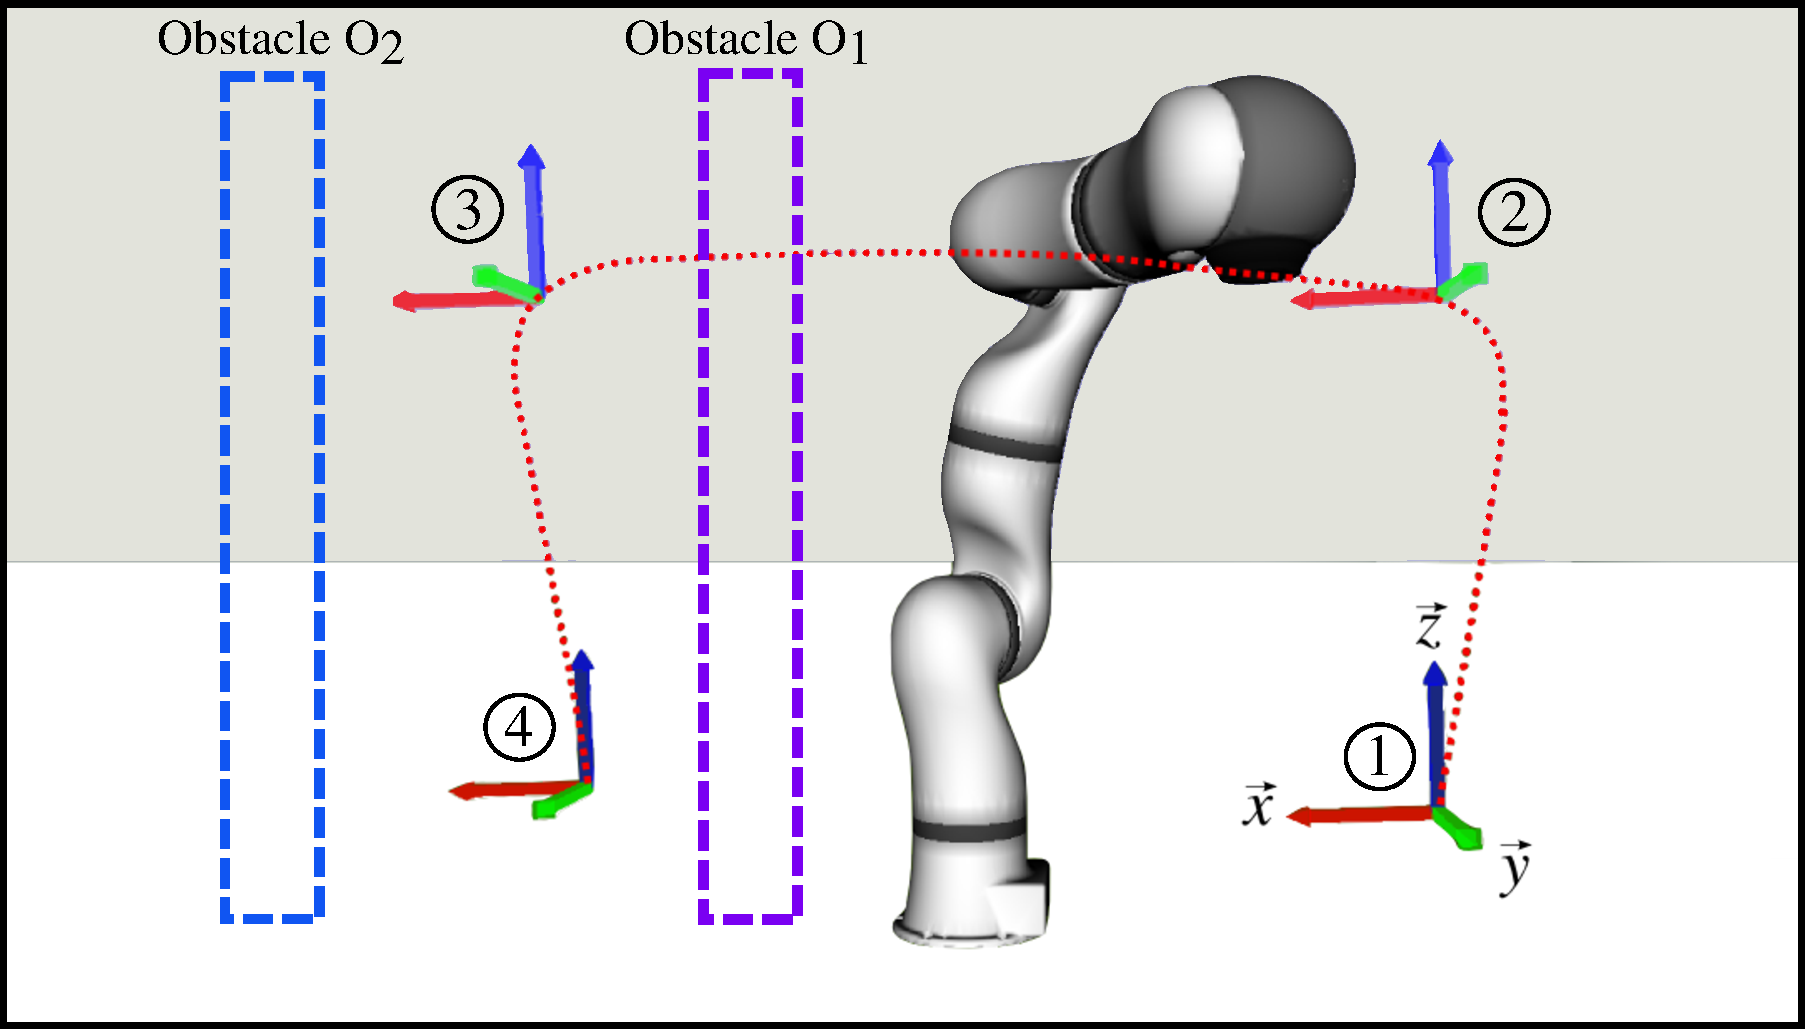
\includegraphics[width=0.8\columnwidth]{\figurepath/kuka_in_xde862301}}
\caption{The KUKA LWR4 robotic manipulator within the XDE simulated world near its considered obstacle. Case $O_1$ is when the obstacle intersects with the trajectory of the robot. Case $O_2$ is when the obstacle is nearby the robot but does not intersect with its trajectory.} 
\label{fig:kuka_in_xde862301_a}
\end{figure}
In the test case scenario, the movement of the robot is not obstructed and the pick and place task is performed with the needed kinetic energy to properly track the desired trajectory $X^*(t)$ in the most optimal way. 
%\begin{figure}[h]
%\centering
%{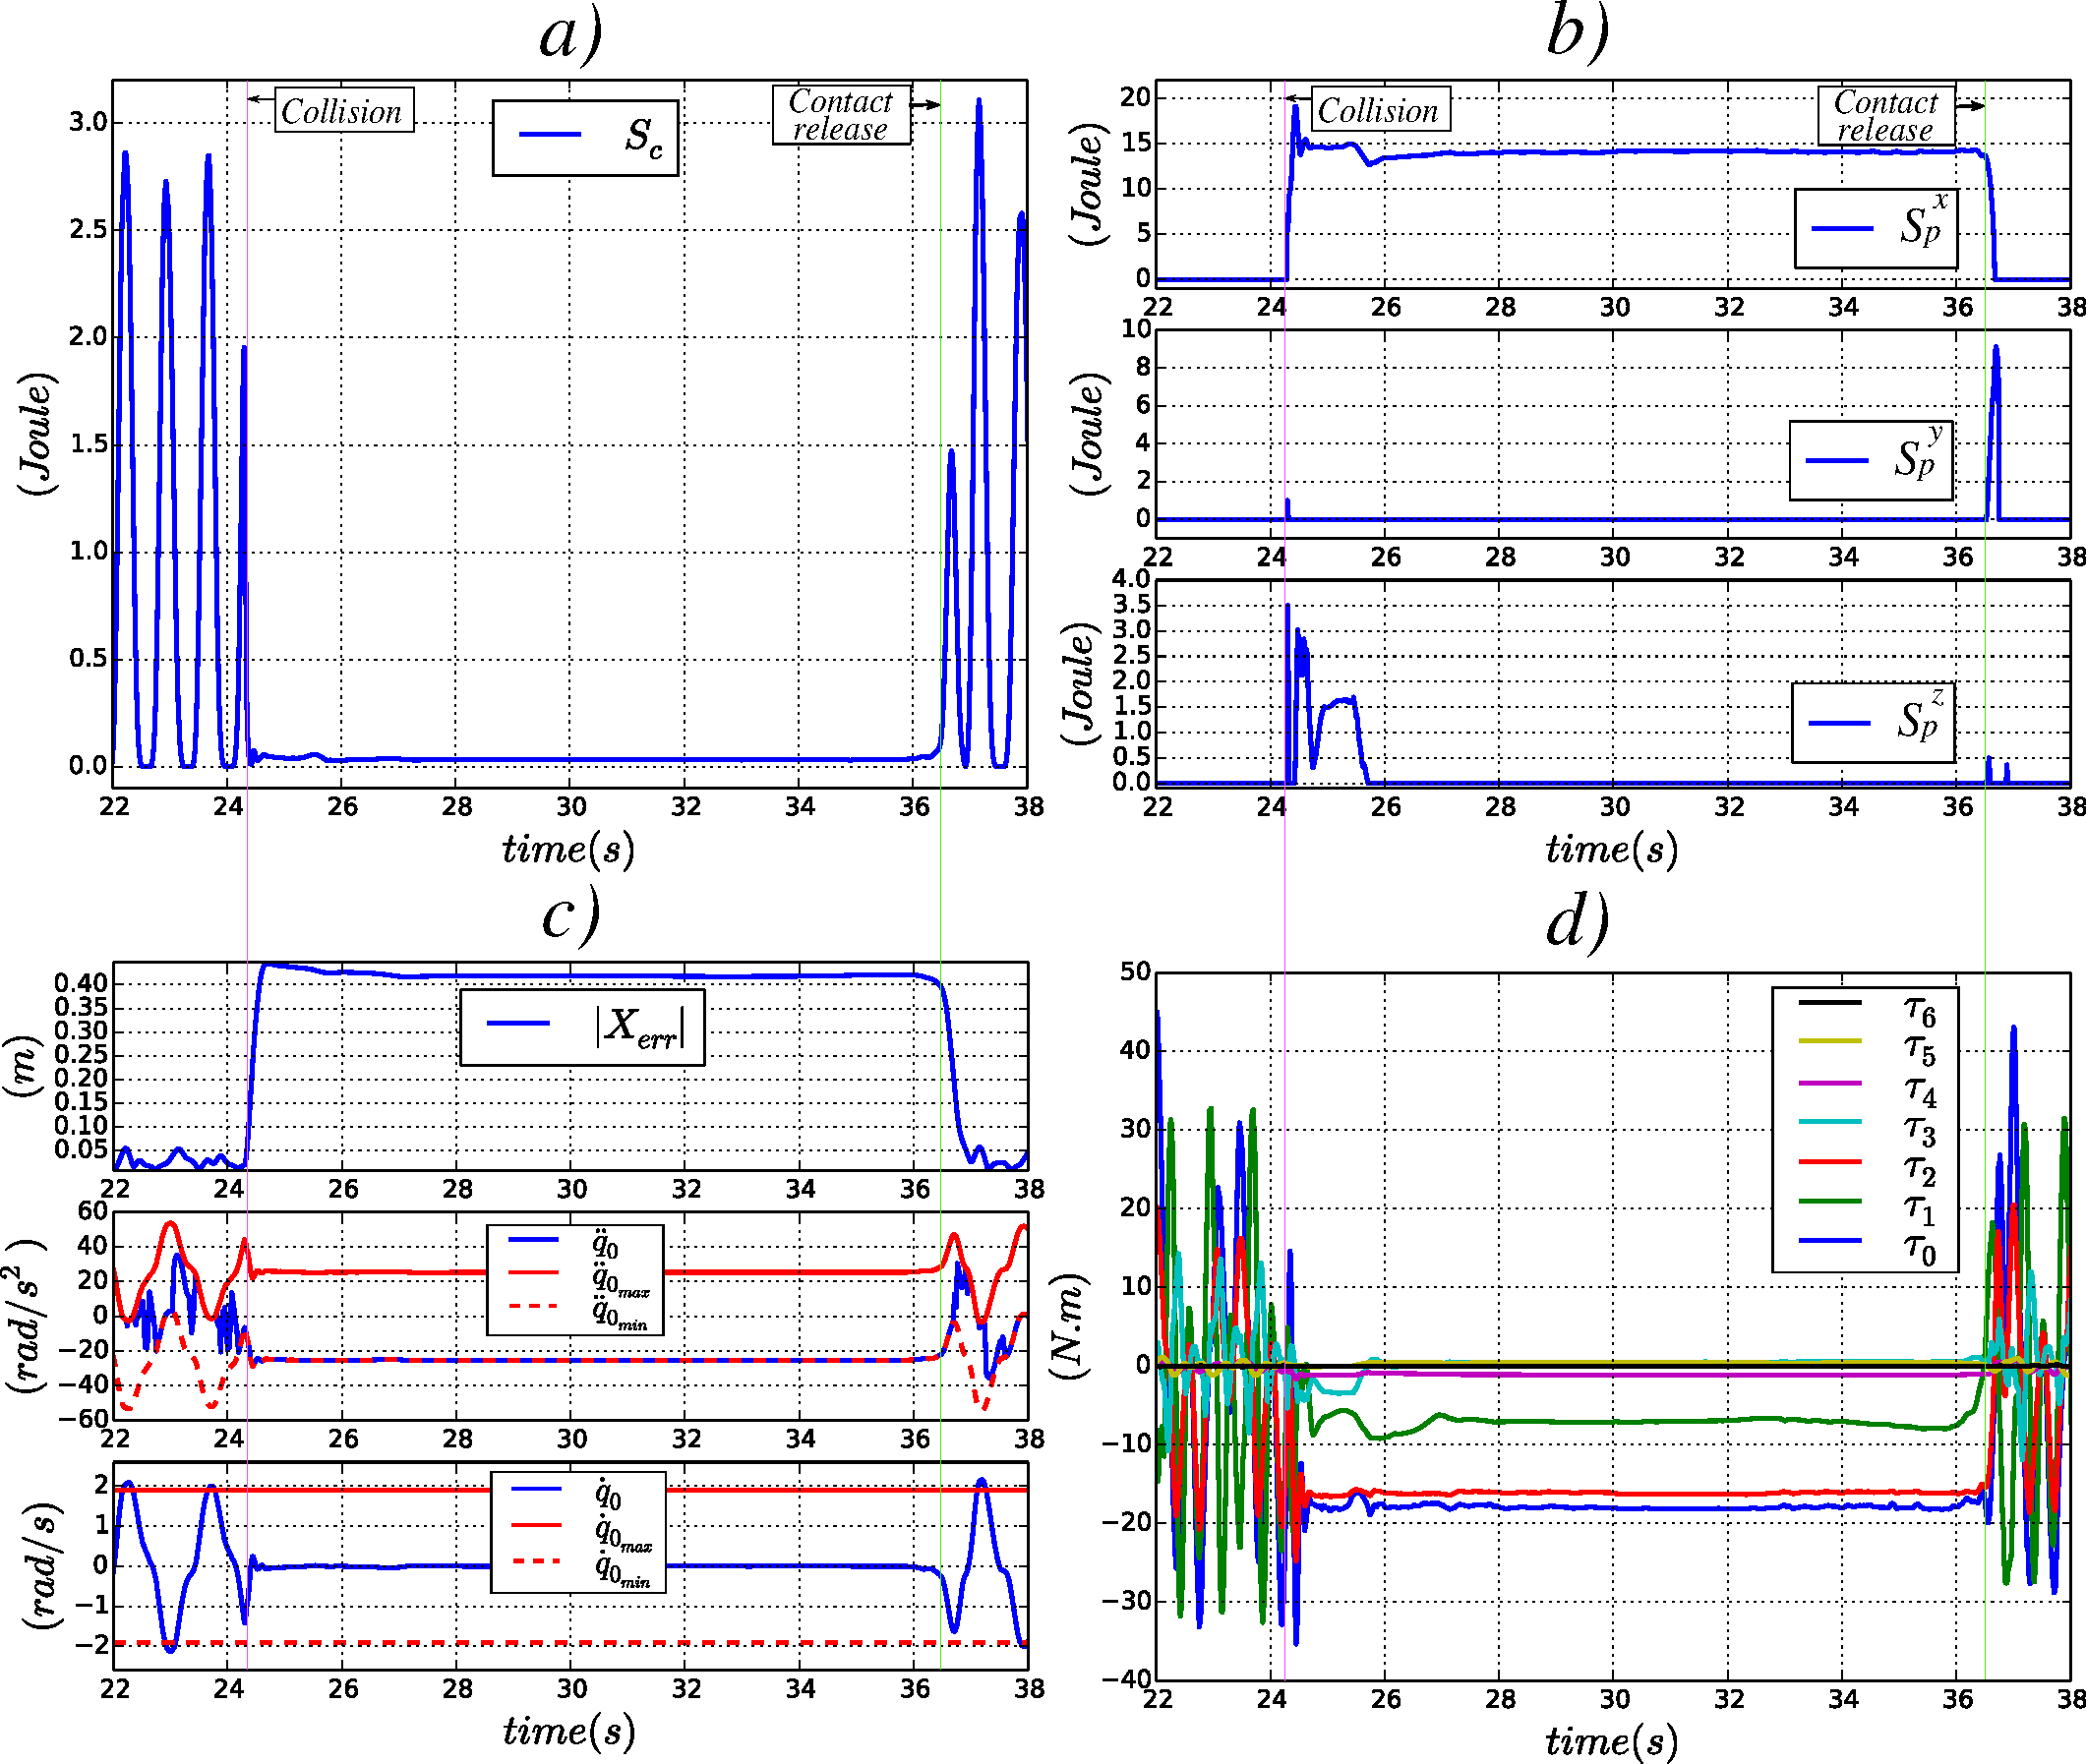
\includegraphics[width=0.7\columnwidth]{\figurepath/vel_track_woO_Ec_woEc}}
%\caption{a): Unconstrained kinetic energy of the end-effector in the direction of a nearby obstacle (case $O_2$ in Fig.~\ref{fig:kuka_in_xde}). b), c) and d): Velocity performance for the  pick and place movement nearby the considered obstacle.} 
%\label{fig:vel_track_woO_woEc}
%\end{figure}
Trajectory tracking performances can be observed in Fig.~\ref{fig:X_Xerr} and Fig.~\ref{fig:k_xdot}.
\begin{figure}[h]
\centering
{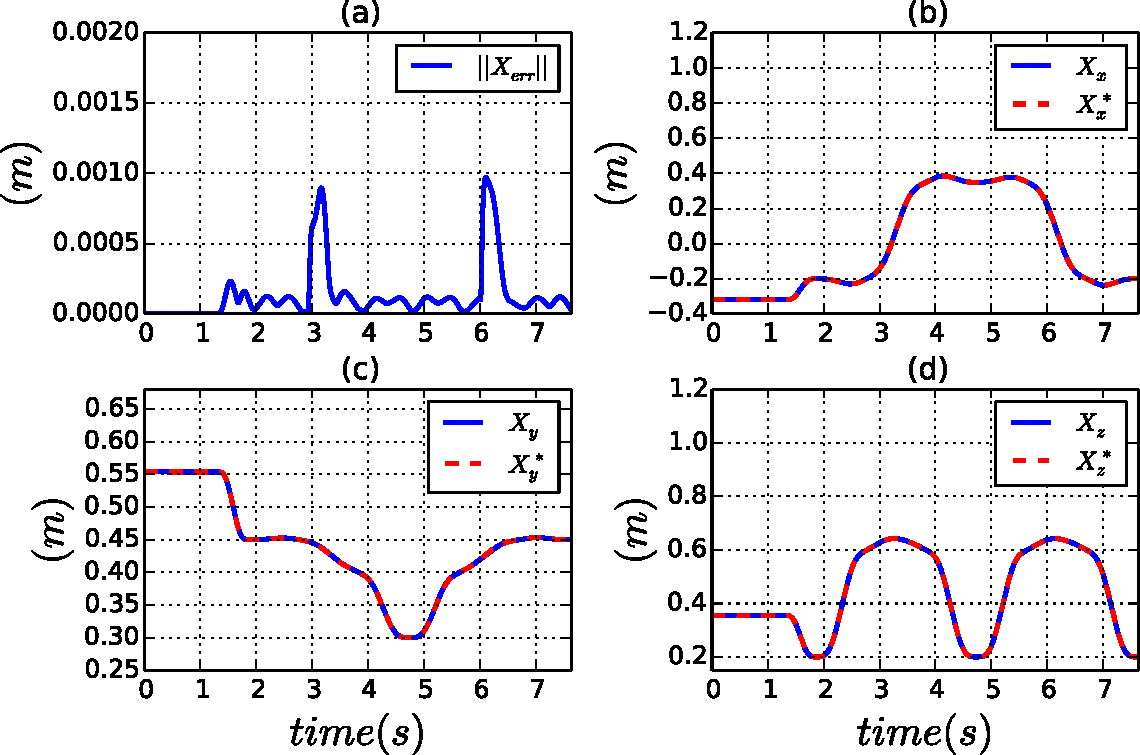
\includegraphics[width=1\columnwidth]{\figurepath/X_Xerr}}
\caption{(a) Norm of the position tracking error for the end-effector of the robot in Cartesian space. (b), (c) and (d) are the real and desired position for the end-effector along the $\vect{x}$, $\vect{y}$ and $\vect{z}$ axis in Cartesian space.} 
\label{fig:X_Xerr}
\end{figure}
\begin{figure}[!htbp]
\centering
{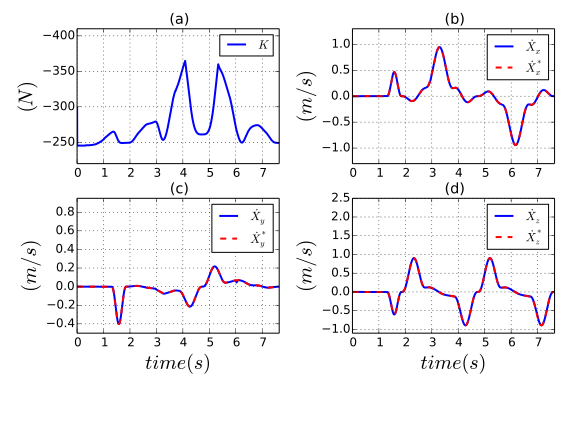
\includegraphics[width=1\columnwidth]{\figurepath/k_xdot}}
\caption{(a) Producible braking force of the robot expressed at the level of its end-effector in the opposite direction to the considered obstacle (case $O_2$ in Fig.~\ref{fig:kuka_in_xde862301_a}). (b), (c) and (d) are the instantaneous real and desired velocities along the $\vect{x}$, $\vect{y}$ and $\vect{z}$ axis in Cartesian space.} 
\label{fig:k_xdot}
\end{figure}
Maximum tracking errors in Cartesian space are: $1 \times 10^{-3}~m$ for position and $2.3 \times 10^{-2}~rad$ for orientation. 

One of the main advantages of using a QP to compute the actuation torque is the possibility to take into account the physical limitations of the system.  Fig.~\ref{fig:q_qdot} and Fig.~\ref{fig:tau_qdddot} show how the limits on articular position, velocity, torque and also jerk are satisfied whenever a joint reaches its considered bounds. Along the movement of the robot, articular positions are within their max/min boundaries. And thanks to the new formulation of the constraint on articular velocity ((\ref{eq:cnt_lit_22}) \& (\ref{eq:cnt_lit_22_bis})), the compatibility with the constraint on articular jerk (\ref{eq:cnt_lit_55}) is ensured. Indeed, when coping with a joint velocity limit (see joint $0$ in Fig.~\ref{fig:q_qdot}.b and Fig.~\ref{fig:tau_qdddot}.b), maximum producible jerk is used to bring the articular acceleration to zero. More details about this new formulation of the joint velocity constraint can be found in Chapter~\ref{chap:Constrcomp}, Subsection~\ref{subsec:jnt_vel_cnstr_inc_jerk}.
\begin{figure}[!htbp]
\centering
{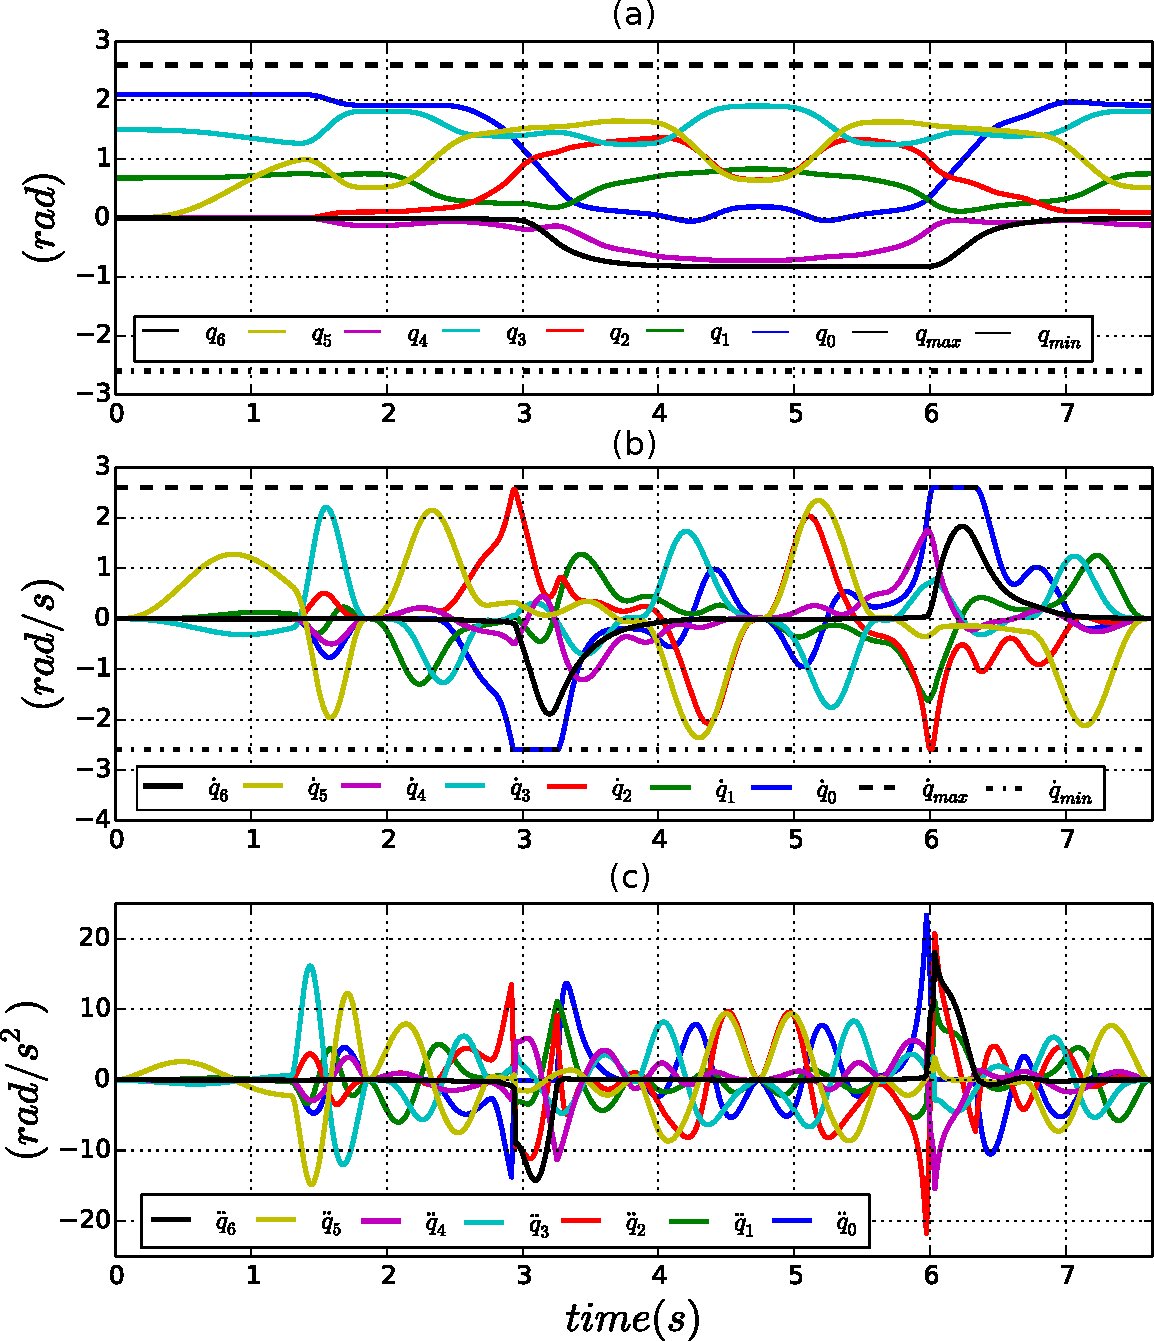
\includegraphics[width=0.90\columnwidth]{\figurepath/q_qdot}}
\caption{Articular position, velocity and acceleration that correspond to the pick and place movement when the energy of the robot is not constrained.} 
\label{fig:q_qdot}
\end{figure}
%\begin{figure}[!htbp]
%\centering
%{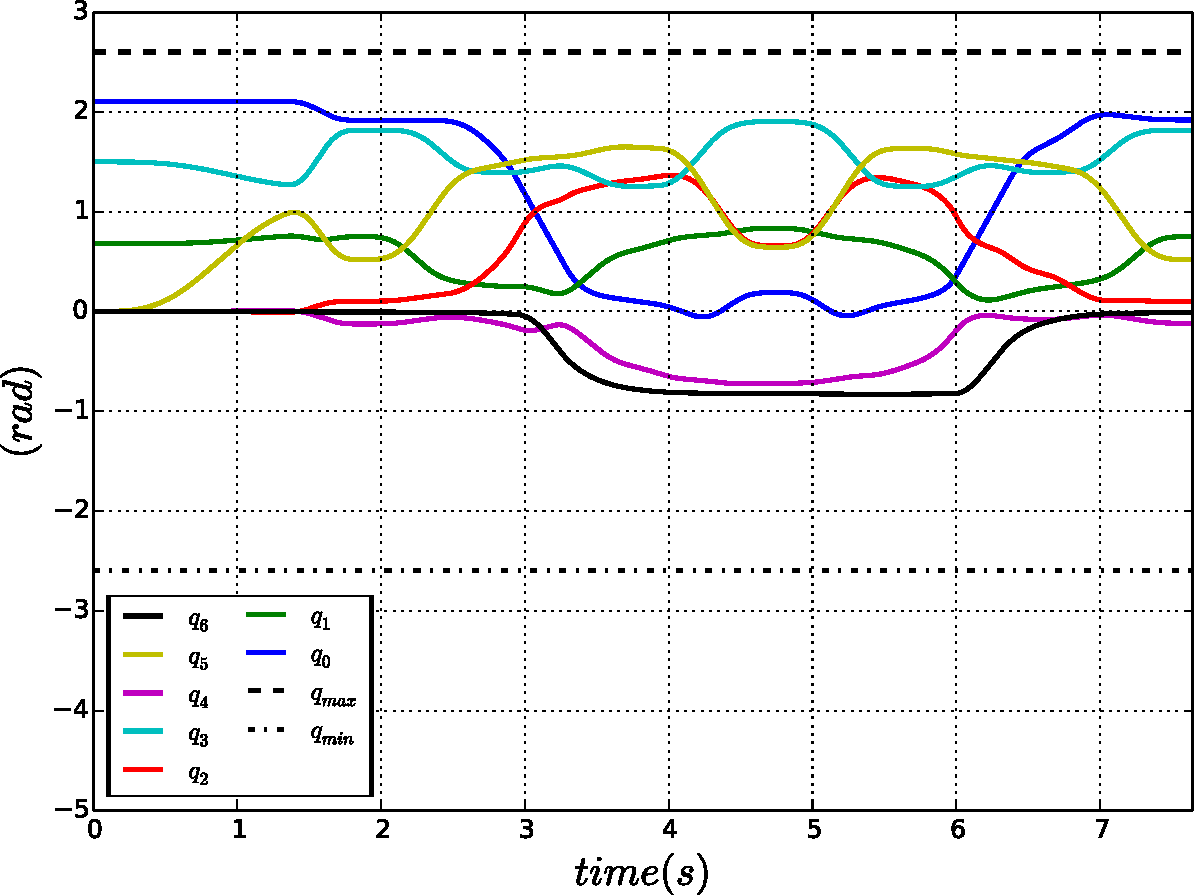
\includegraphics[width=0.8\columnwidth]{\figurepath/q}}
%\caption{4} 
%\label{fig:q}
%\end{figure}
%\begin{figure}[!htbp]
%\centering
%{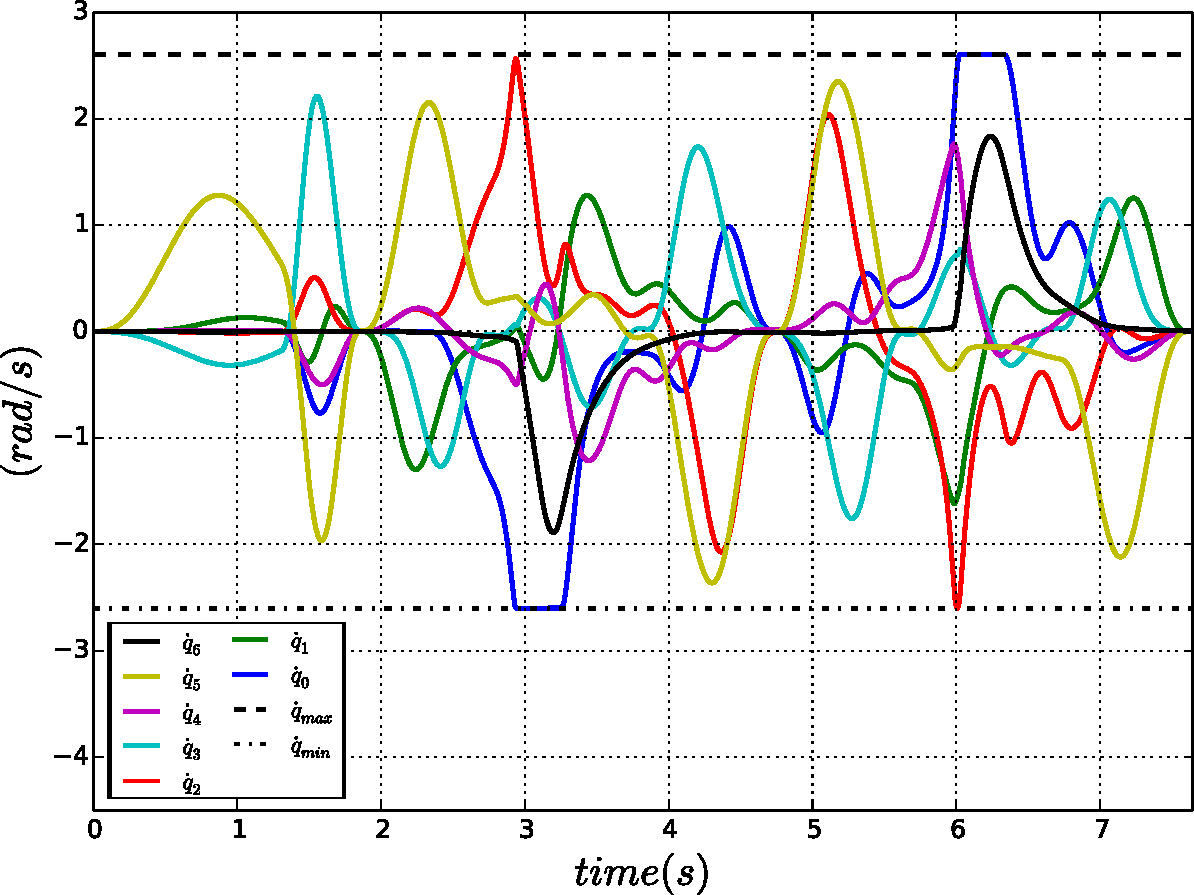
\includegraphics[width=0.8\columnwidth]{\figurepath/qdot}}
%\caption{5} 
%\label{fig:qdot}
%\end{figure}
%\begin{figure}[!htbp]
%\centering
%{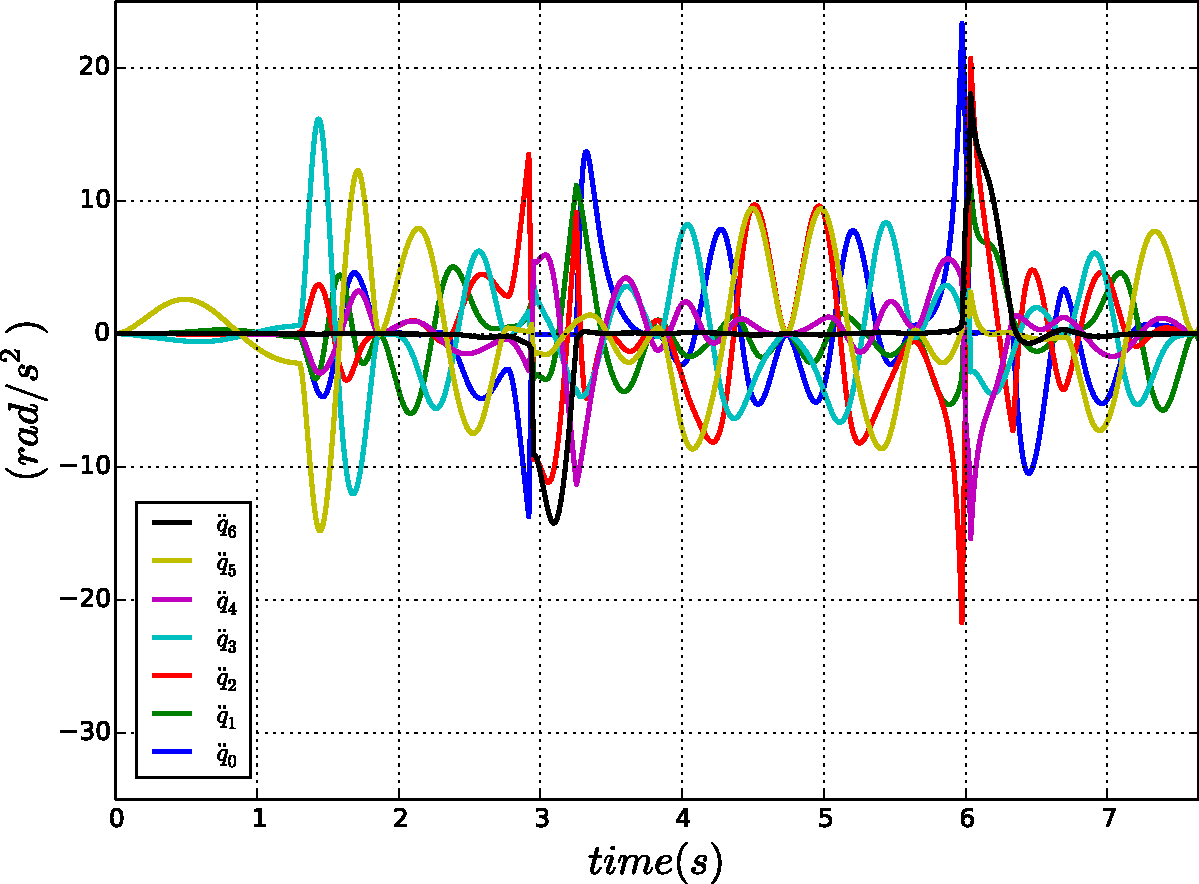
\includegraphics[width=0.8\columnwidth]{\figurepath/qdotdot}}
%\caption{6} 
%\label{fig:qdotdot}
%\end{figure}
\begin{figure}[!htbp]
\centering
{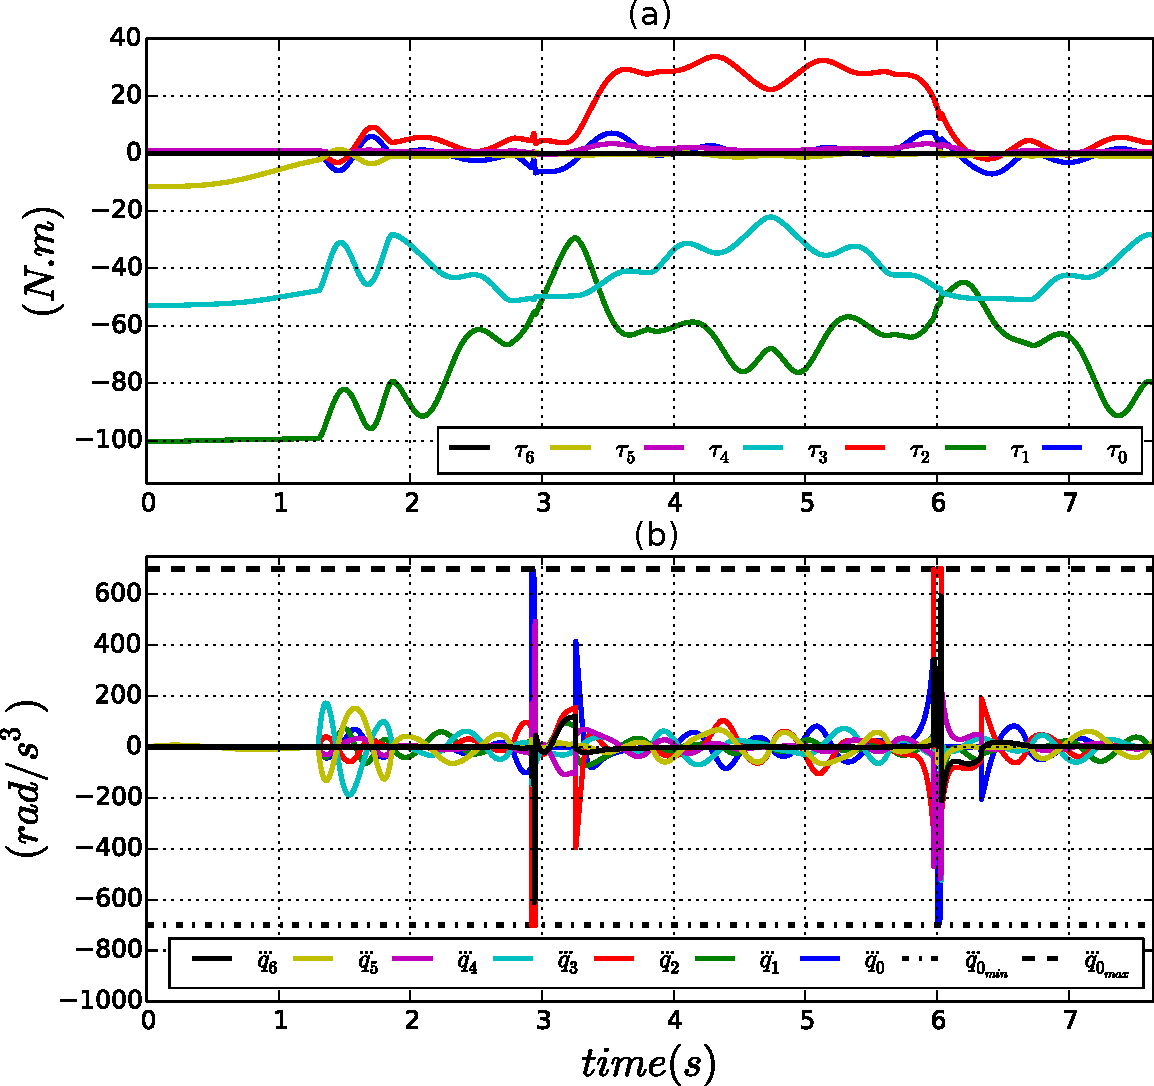
\includegraphics[width=0.90\columnwidth]{\figurepath/tau_qdddot}}
\caption{Articular torque and jerk that correspond to the pick and place movement when the energy of the robot is not constrained.} 
\label{fig:tau_qdddot}
\end{figure}
%\begin{figure}[!htbp]
%\centering
%{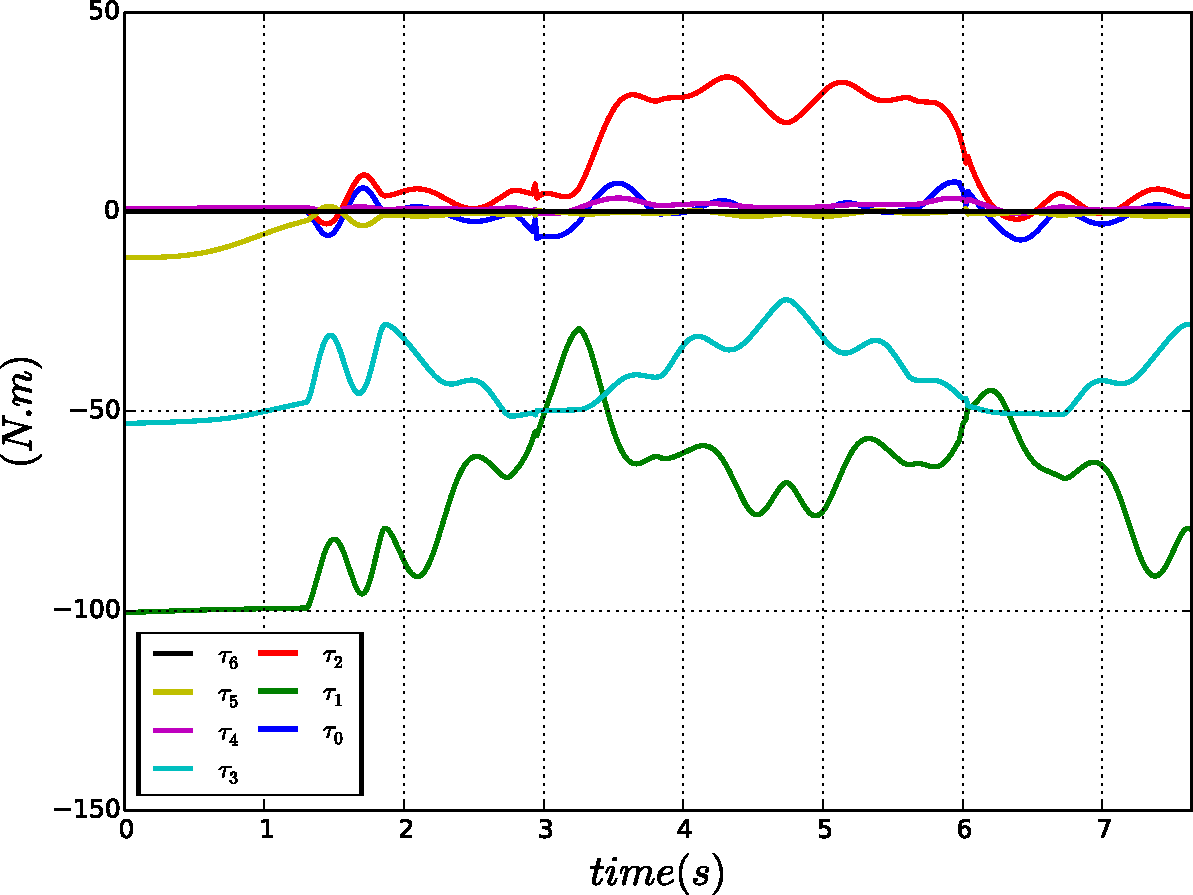
\includegraphics[width=0.8\columnwidth]{\figurepath/tau}}
%\caption{7} 
%\label{fig:tau}
%\end{figure}
%\begin{figure}[!htbp]
%\centering
%{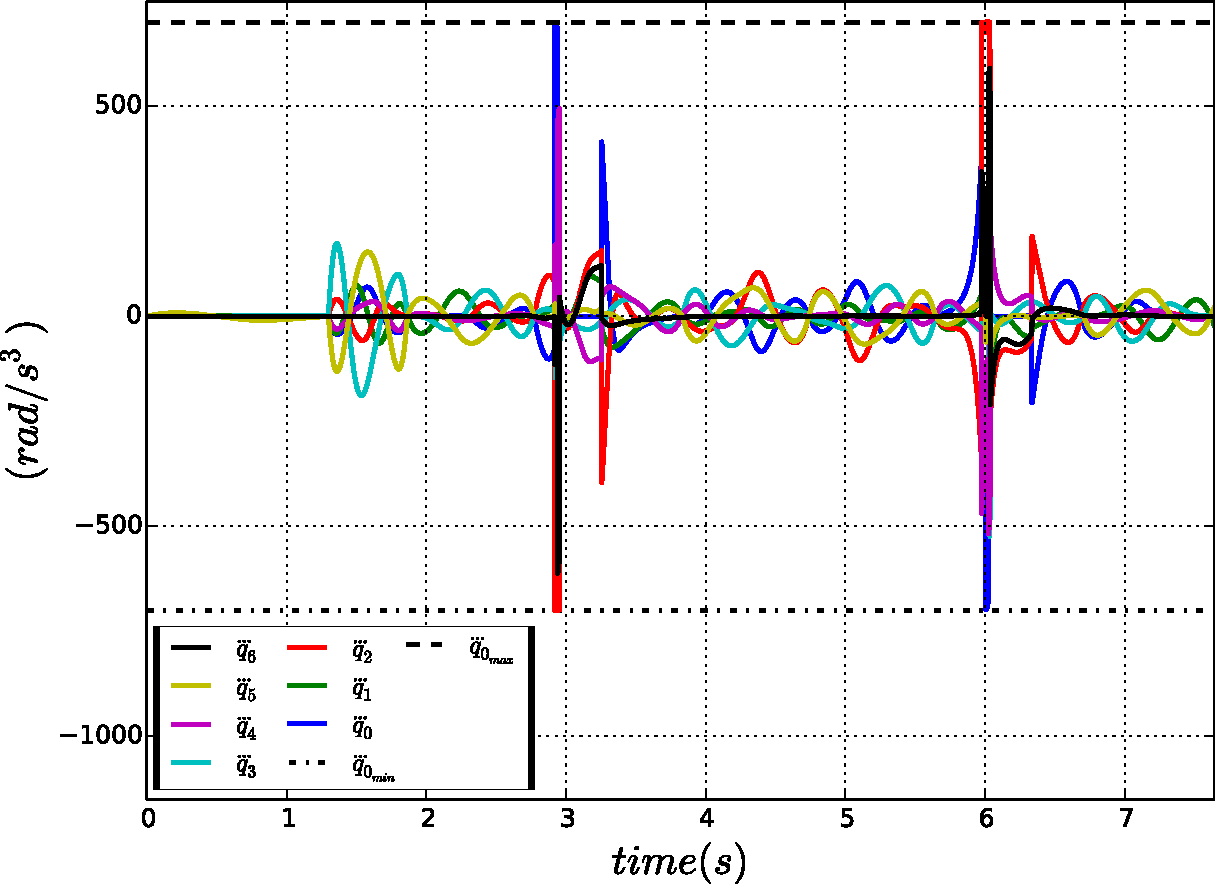
\includegraphics[width=0.8\columnwidth]{\figurepath/qdotdotdot_!!!!}}
%\caption{8} 
%\label{fig:qdotdotdot_!!!!}
%\end{figure}
%\\
%\begin{figure}[h]
%\centering
%{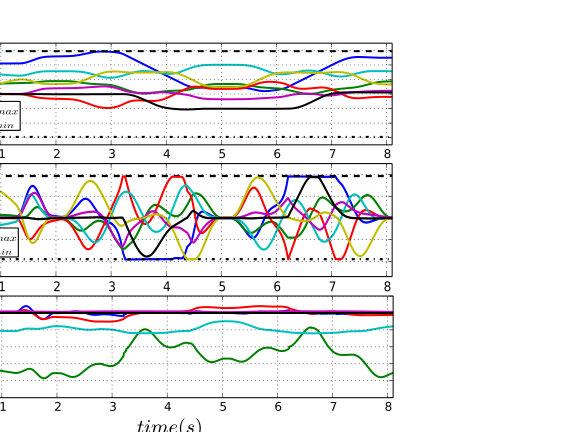
\includegraphics[width=0.7\columnwidth]{\figurepath/art_data_woO_woEc}}
%\caption{Articular positions, velocity and torque of the  pick and place movement without constraint on the kinetic energy of the end-effector.} 
%\label{fig:art_data_woO_woEc}
%\end{figure}
\\
The trajectory of the robot in this scenario does not intersect with any obstacle. During this \textit{free movement}, a number of parameters related to the dynamic capabilities of the robot in operational space and to the accomplished task are registered. Fig.~\ref{fig:k_xdot}.a illustrates the instantaneous producible equivalent braking force in Cartesian space expressed at the level of the end-effector in the opposite direction to the nearby obstacle (case $O_2$ in Fig.~\ref{fig:kuka_in_xde862301_a}). This force depends on the instantaneous articular configuration $\vect{q}_{|k}$ and on the amount of torque producible by the actuators of the robot. $K$ is computed as described in (\ref{eq:K_maximizing_opt}) and its minimum guaranteed value along this movement will be used to synthesise the kinetic energy based safety criteria introduced in (\ref{eq:k_fd}). Fig.~\ref{fig:k_xdot}.b, c and d depict how the desired velocity $\vect{\dot{X}}^*(t)$ of the end-effector of the robot is properly tracked in real-time. 
Kinetic energy of the KUKA LWR4, expressed at its end-effector and generated in the direction of the nearby considered obstacle (case $O_2$ in Fig.~\ref{fig:kuka_in_xde862301_a}) is shown in Fig.~\ref{fig:energy_profile}.a. Its maximum value is $2.15~J$; which is equivalent to a $5~kg$ mass, moving at $0.92~m/s$.
At every time-step, the plotted kinetic energy is computed using two different formulations:
\begin{equation}
S_c = E_{c_{|k}}^{EE,O} = \frac{1}{2} m(\vect{q}_{|k})_{EE,O}^{eq} v_{EE_{|k}}^{{EE,O}^2},
\label{eq:plotted_Sc}
\end{equation}
and: 
\begin{equation}
\begin{split}
S_c = E_{c_{|k}}^{EE,O} = \sum\limits_{n=1}^{k-1} S_{p_{free_{|n}}} =  \sum\limits_{n=1}^{k-1} m(\vect{q}_{|n})_{EE,O}^{eq} \ddot{X}_{EE_{|n}}^{EE,O} \left(\vect{X}_{EE_{|n+1}} - \vect{X}_{EE_{|n}}\right) \vect{n}_O.
\end{split}
\label{eq:plotted_Sc2}
\end{equation}
Fig.~\ref{fig:energy_profile}.a illustrates how the kinetic energy of the robot at time-step $k$ is indeed equal (errors aside) to the sum of all the previously \textit{injected} potential energies.
%the small difference between the two curves is mainly due to the variation of the articular configuration between two successive control time-steps: $n$ and $n+1$; the Jacobian and equivalent mass are not considered at the same time-step.
\begin{figure}[!htbp]
\centering
{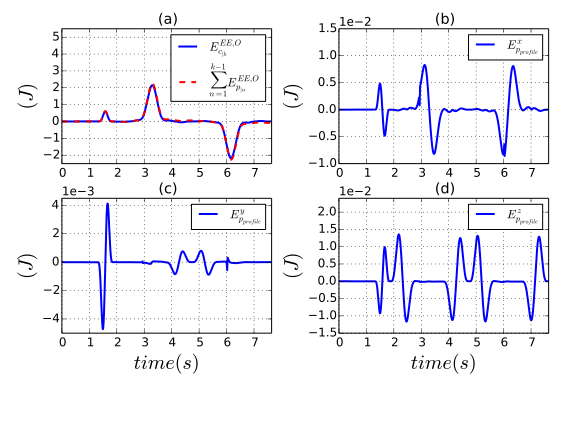
\includegraphics[width=1\columnwidth]{\figurepath/energy_profile}}
\caption{(a) Kinetic energy of the robot in the direction of the considered obstacle (case $O_2$ in Fig.~\ref{fig:kuka_in_xde862301_a}), computed using (\ref{eq:plotted_Sc}) and (\ref{eq:plotted_Sc2}) during the pick and place movement. (b), (c) and (d) are the energy profiles that correspond to the pick and place task along the $\vect{x}$, $\vect{y}$ and $\vect{z}$ axis in Cartesian space.} 
\label{fig:energy_profile}
\end{figure}
%%%%%%%%%%%%%%%%%%%%%%%%%%SUBSECTION%%%%%%%%%%%%%%%%%%%%%%%%%%%%%
%%%%%%%%%%%%%%%%%%%%%%%%%%%%%%%%%%%%%%%%%%%%%%%%%%%%%%%%%%%%%%%%%
%%%%%%%%%%%%%%%%%%%%%%%%%%SUBSECTION%%%%%%%%%%%%%%%%%%%%%%%%%%%%%
\subsection{Scenario 1: obstacle intersecting with the trajectory of the robot and no constraints on its energy} \label{subsec_no_constr_energy}
In this scenario, the obstacle intersects with the \circled{2}-\circled{3} segment of the pick and place movement (case $O_1$ in Fig.~\ref{fig:kuka_in_xde862301_a}). When collision occurs between the robot and the rigid object, most of its kinetic energy is rapidly dissipated. Fig.~\ref{fig:ec_obst3!!!!} shows how $1.66~J$ of this kinetic energy are instantaneously dissipated at impact. 
%\begin{figure}[h]
%\centering
%{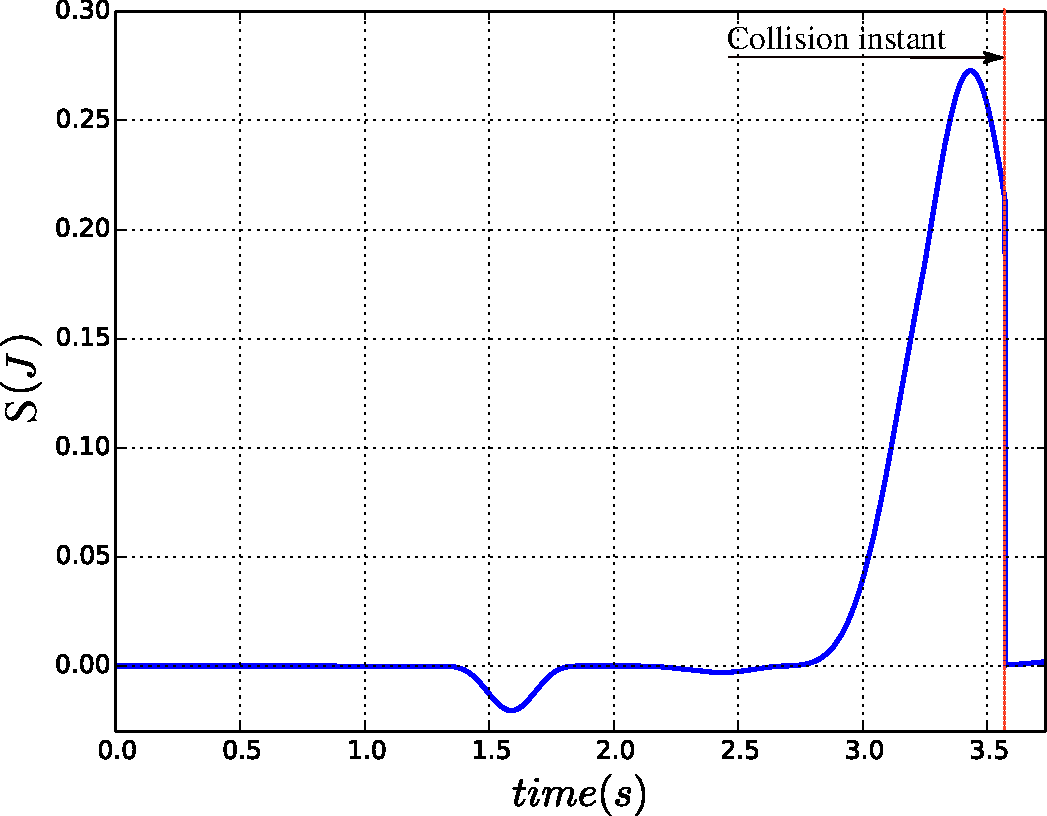
\includegraphics[width=0.5\columnwidth]{\figurepath/Ke_wO_wC_woEc}}
%\caption{Dissipation of the unconstrained kinetic energy of the robot end-effector in the direction of the considered obstacle during collision.} 
%\label{fig:Ke_wO_wC_woEc}
%\end{figure}
\begin{figure}[!htbp]
\centering
{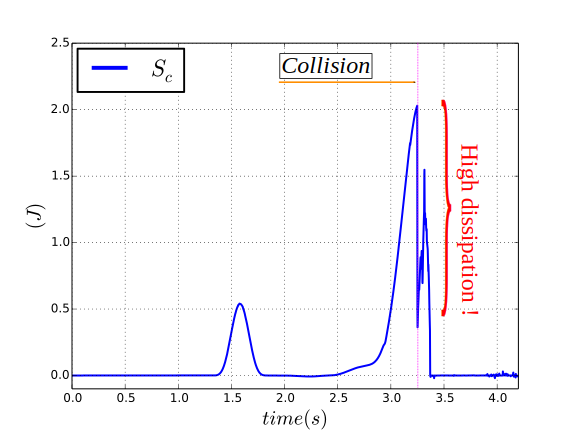
\includegraphics[width=0.75\columnwidth]{\figurepath/ec_obst3!!!!}}
\caption{Kinetic energy of the KUKA LWR4 expressed at the level of its end-effector in the direction of the considered obstacle during, at and after collision.} 
\label{fig:ec_obst3!!!!}
\end{figure}
According to (\ref{eq:Energydissipationmodel1}) and as can be seen in  Fig.~\ref{fig:ep__f_tau_!!!!}.b, this fast dissipation induces a large impact force of $551~N$. Which could clearly damage the collided obstacle or the robot. In this simulation and also in all the upcoming ones, a force sensor is linked to the base of the collided object (i.e., the wall). The main impact force is along the $\vect{x}$ axis (see Fig.~\ref{fig:kuka_in_xde862301_a}), which is the main direction of movement of the end-effector of the robot before collision.
% and thus, the controller can be considered unsafe.   
%\begin{figure}[!htbp]
%\centering
%{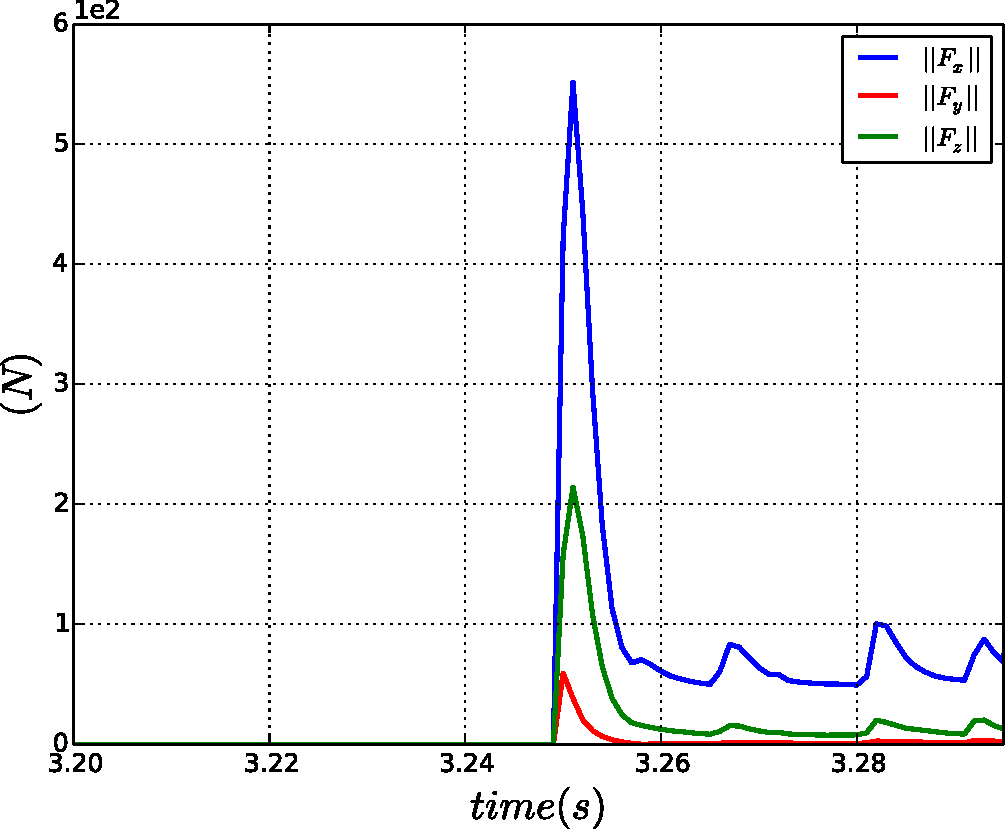
\includegraphics[width=0.8\columnwidth]{\figurepath/force_sensor2}}
%\caption{10} 
%\label{fig:force_sensor2}
%\end{figure}
\begin{figure}[!htbp]
\centering
{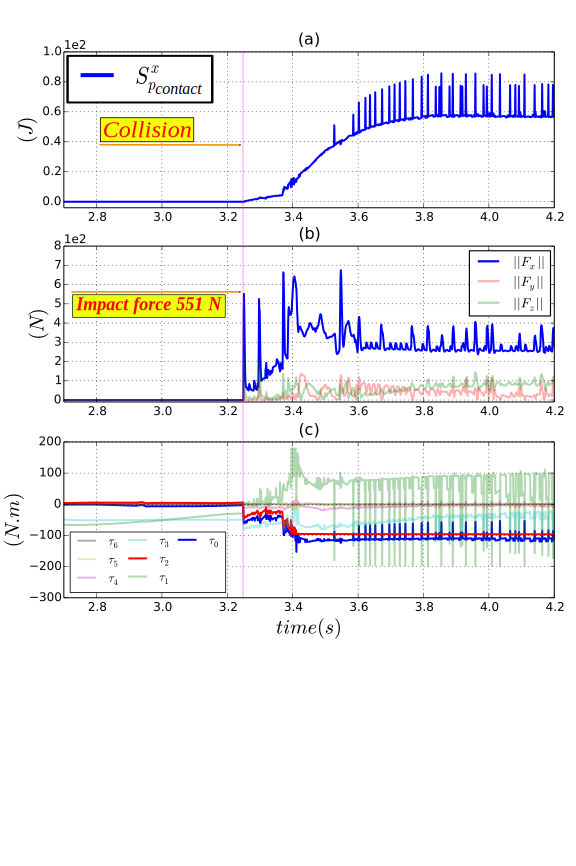
\includegraphics[width=0.90\columnwidth]{\figurepath/ep__f_tau_!!!!}}
\caption{(a) \textit{Potential energy} accumulated in the controller of the robot during physical contact along the $\vect{x}$ axis in Cartesian space. (b) Contact forces between the robot and the wall after the establishment of physical contact along the $\vect{x}$, $\vect{y}$ and $\vect{z}$ axis in Cartesian space. (c) Actuation torques during physical contact with the considered obstacle.} 
\label{fig:ep__f_tau_!!!!}
\end{figure}
After the peak of force corresponding to the first collision, physical contact between the robot and the wall is established. As this obstacle obstructs the movement of the KUKA LWR4, the divergence between the desired and real positions for its end-effector causes the augmentation of the amount of \textit{potential energy} that accumulates in the controller of the robot (see Fig.~\ref{fig:ep__f_tau_!!!!}.a). Consequently, the resulting contact force along the $\vect{x}$ axis also intensifies. \\
%\begin{figure}[!htbp]
%\centering
%{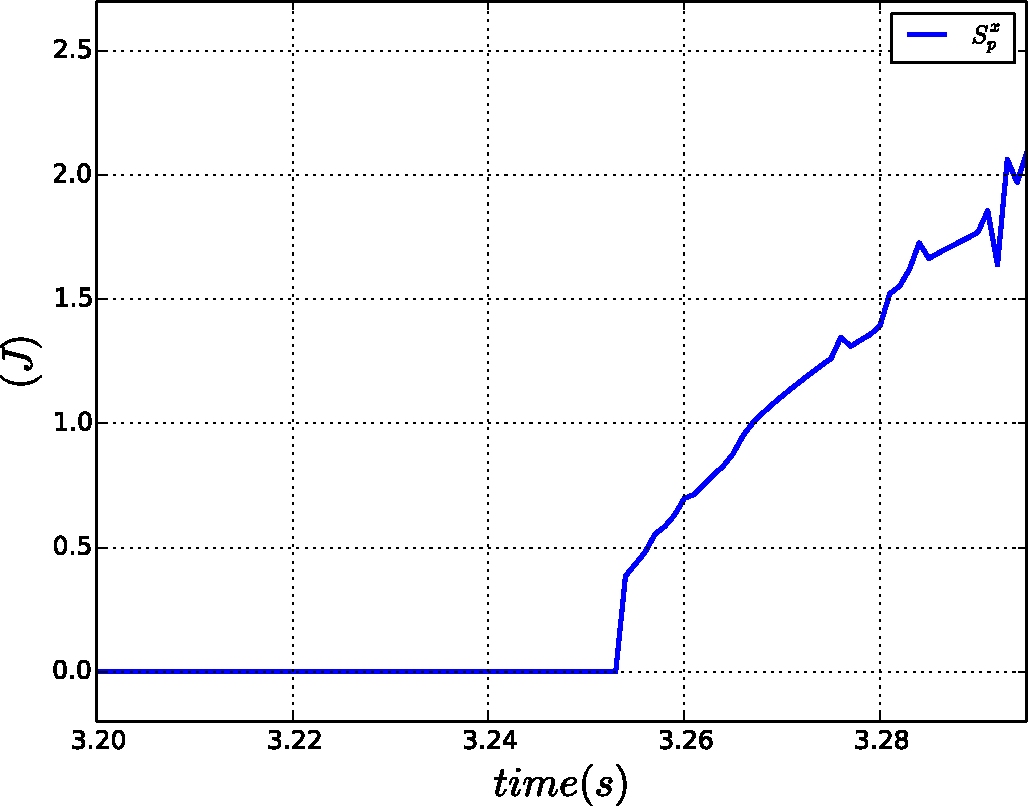
\includegraphics[width=0.8\columnwidth]{\figurepath/Ep_contact_selon_x_seul_!!!!}}
%\caption{11} 
%\label{fig:Ep_contact_selon_x_seul_!!!!}
%\end{figure}
%\begin{figure}[!htbp]
%\centering
%{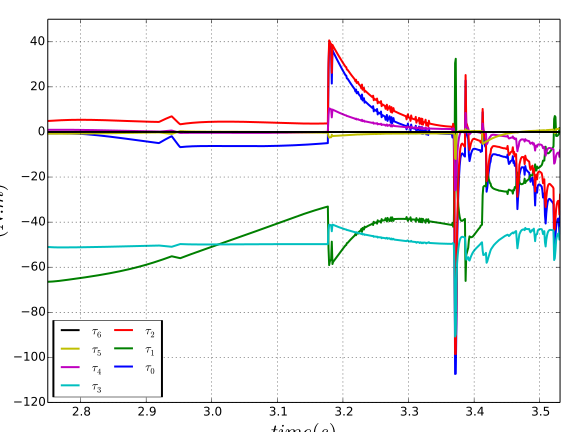
\includegraphics[width=0.8\columnwidth]{\figurepath/tau2}}
%\caption{12} 
%\label{fig:tau2}
%\end{figure}
The contact force along the $\vect{x}$ axis is mainly caused by the torques generated by joint $0$ and joint $2$. Fig.~\ref{fig:ep__f_tau_!!!!}.c shows how $\tau_0$ and $\tau_2$ increase to respectively reach $\approx -115~N.m$ and $\approx -95~N.m$\footnote{In the configuration of the robot as seen in Fig.~\ref{fig:kuka_in_xde862301_a}, negative torque on joint $0$ and on joint $2$ causes the end-effector of the robot to move towards the wall. Positive torque makes it move in the opposite direction.}. As depicted in Fig.~\ref{fig:ep__f_tau_!!!!}.b, the contact force that correspond to these generated torques settles around $250~N$. The \textit{potential energy} that accumulates in the controller of the robot and the contact force derived from it stop increasing when the desired position for the end-effector stops diverging once at point \circled{3} from the \circled{2}-\circled{3} segment (see Fig.~\ref{fig:kuka_in_xde862301_a}).\\
Clearly, considering the big amounts of generated impact and contact forces, the controller with its current configuration is not appropriate for enabling \textit{safe} physical interaction between the robot and its environment. Therefore, the introduced energy related constraints should be included for the upcoming configurations.
%%%%%%%%%%%%%%%%%%%%%%%%%%SUBSECTION%%%%%%%%%%%%%%%%%%%%%%%%%%%%%
%%%%%%%%%%%%%%%%%%%%%%%%%%%%%%%%%%%%%%%%%%%%%%%%%%%%%%%%%%%%%%%%%
%%%%%%%%%%%%%%%%%%%%%%%%%%SUBSECTION%%%%%%%%%%%%%%%%%%%%%%%%%%%%%
\subsection{Scenario 2: nearby obstacle not intersecting with the trajectory of the robot and constraint on its kinetic energy} \label{subsec:no_inter_constr_Ec}
In this case, the first formulation of the kinetic energy related constraint (\ref{eq:Safe_constr_1}) is included in the configuration of the controller to safely account for the presence of a nearby obstacle (i.e., the wall, case $O_2$ in Fig.~\ref{fig:kuka_in_xde862301_a}). This constraint limits the actuation torques and, according to (\ref{eq:S_2}), has a direct impact on the velocity of the end-effector. Depending on how the controller parameters $d_{safe}$, $E_{c_{safe}}$ and $K$ are fixed, physical contact can be allowed or prevented. For example, fixing $d_{safe}=2$ and $E_{c_{safe}} = 0$ forces the end-effector of the robot to stop at $2~m$ from the obstacle. In this scenario, as shown in Fig.~\ref{fig:kuka_xde_nearby_obst}, the obstacle does not intersect with the trajectory of the pick and place movement. In addition to the constraint on the amount of kinetic energy generated in the direction of obstacle $O_2$, the controller is implemented with the inequality constraints that correspond to the articular physical limitations of the actuators of the robot(\ref{eq:const_1_literature1}). Because of possible \textit{incompatibility problems}, the constraint (\ref{eq:cnt_lit_444}) on the producible articular jerk is omitted from the configuration of the controller whenever the constraint (\ref{eq:Safe_constr_1}) on the kinetic energy of the robot is activated. Finally, the equality constraints (\ref{eq:dyn_eq_aab}) that corresponds to the dynamic model of the robot are also included in the control scheme. Finally, the control parameters are fixed as: $E_{c_{safe}} = 0.1~J$, $K = 5~N$, $d_{safe} = 0.25~m$ and $d_{max} = 0.8~m$.
%\begin{figure}[!htbp]
%\centering
%{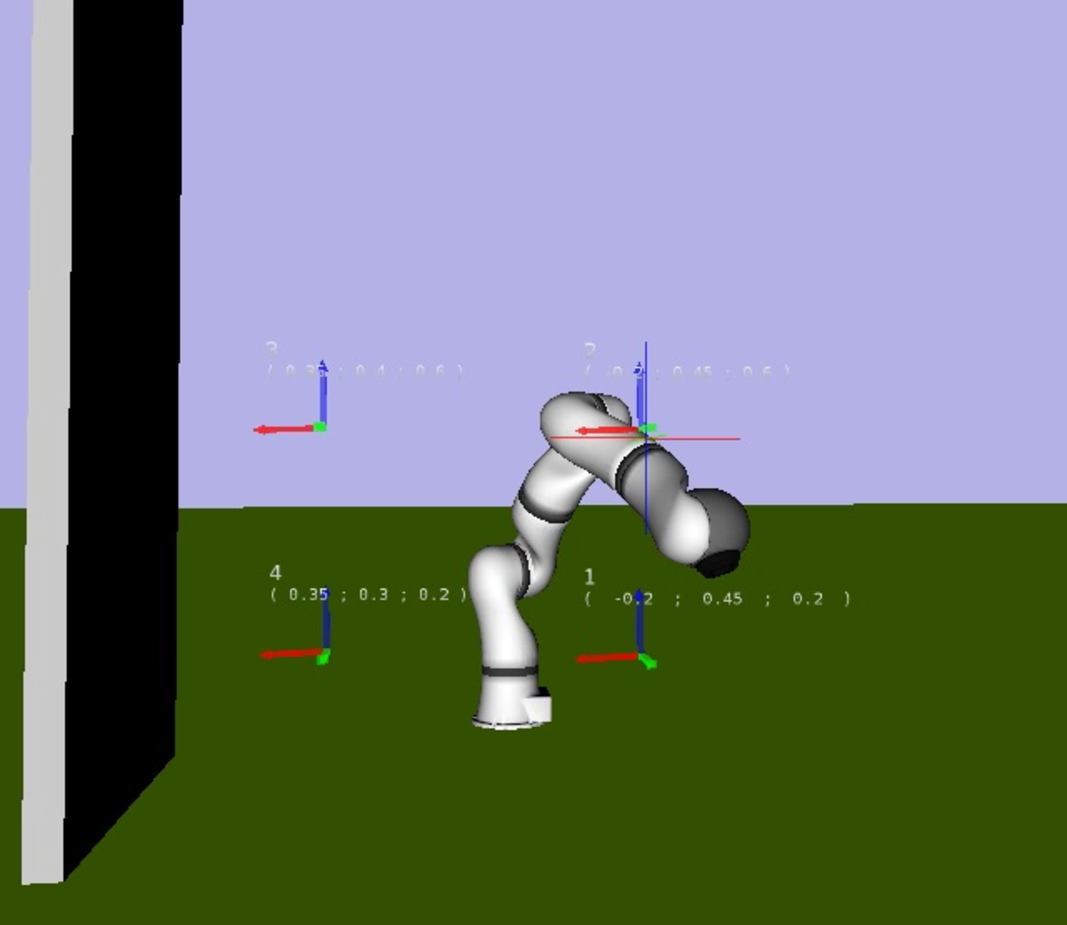
\includegraphics[width=0.55\columnwidth]{\figurepath/kuka_xde_nearby_obst}}
%\caption{11} 
%\label{fig:kuka_xde_nearby_obst}
%\end{figure}
%
%\begin{figure}[!htbp]
%\centering
%{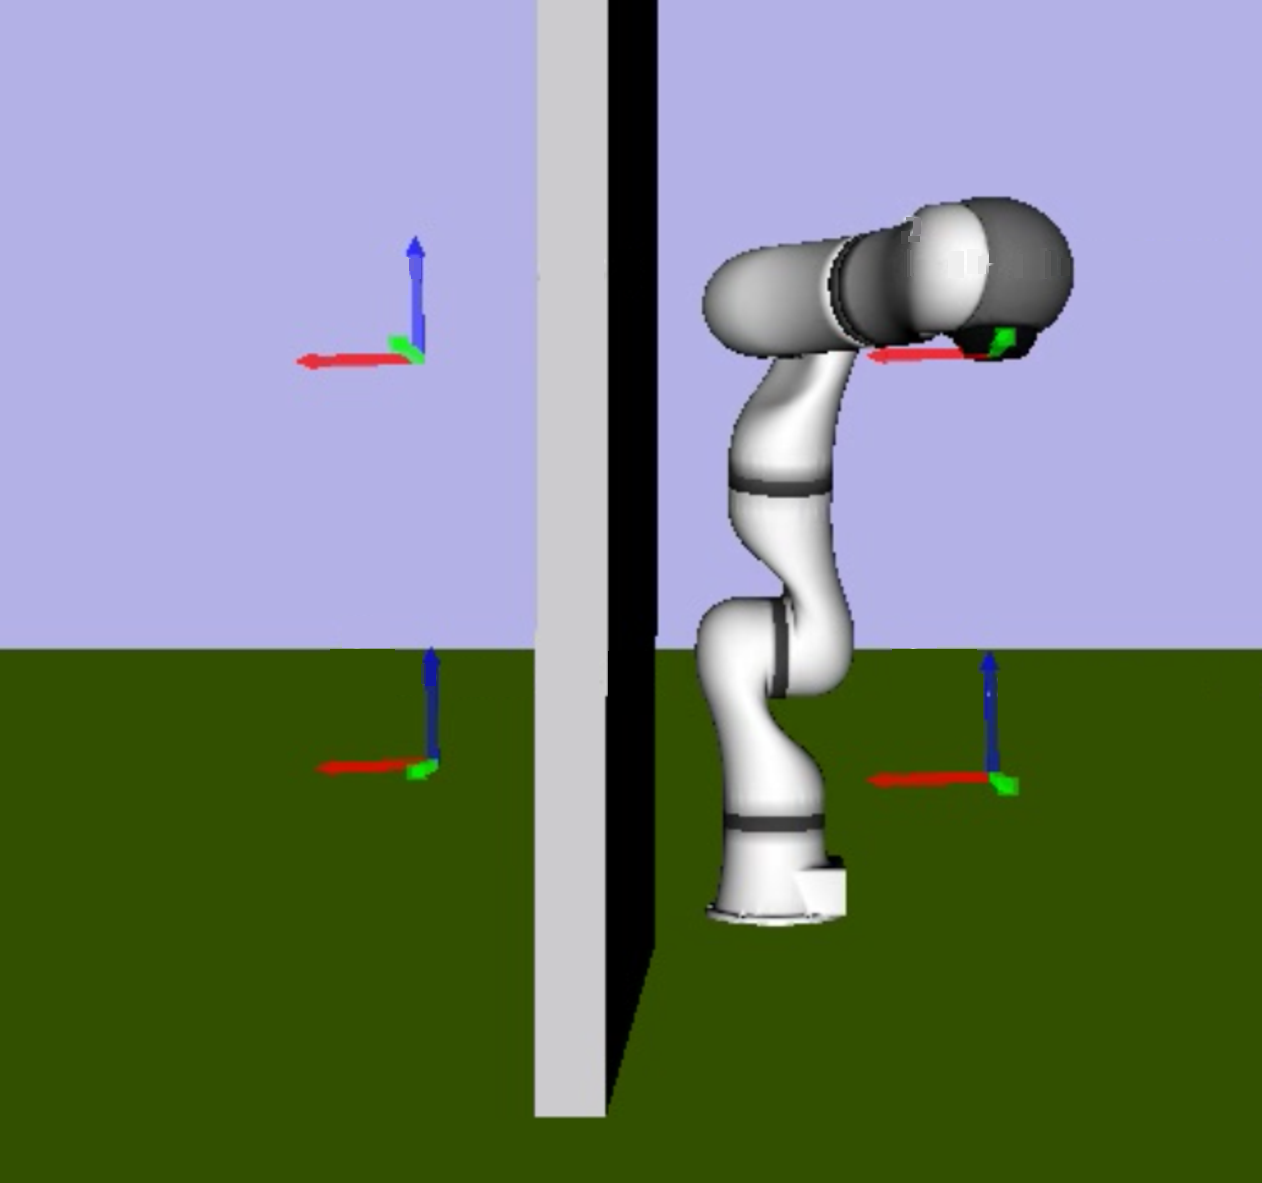
\includegraphics[width=0.65\columnwidth]{\figurepath/screen_shot_kuka_1}}
%\caption{Screen-shot of the KUKA LWR4 robot within the XDE simulator with the wall not intersecting its trajectory.} 
%\label{fig:kuka_xde_nearby_obst}
%\end{figure}
%
\begin{figure}
\begin{minipage}[c]{0.48\linewidth}
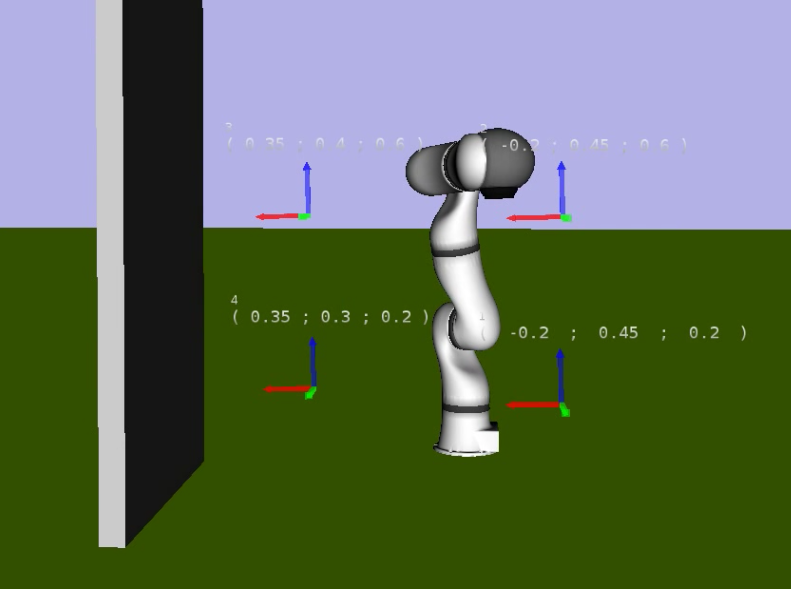
\includegraphics[width=1\columnwidth]{\figurepath/kuka_xde_no_intersect_front_view}
\caption{Screen-shot of the KUKA LWR4 robot within the XDE simulated world with the nearby wall not intersecting its trajectory.} 
\label{fig:kuka_xde_nearby_obst}
\end{minipage}
\hfill
\begin{minipage}[c]{0.48\linewidth}
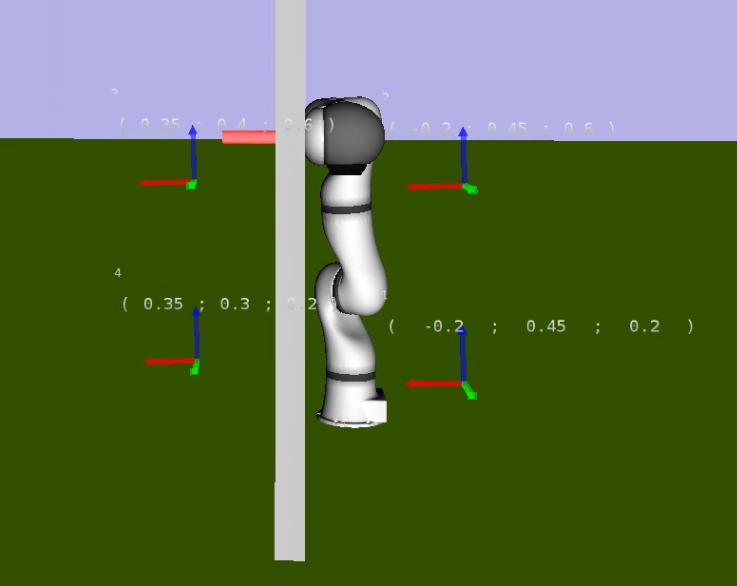
\includegraphics[width=1\columnwidth]{\figurepath/kuka_xde_intersect_front_collision}
\caption{Screen-shot of the KUKA LWR4 robot within the XDE simulator during a collision with the wall intersecting its trajectory.} 
\label{fig:kuka_xde_obst_coll}
\end{minipage}%
\end{figure}
\\
With this particular configuration of its controller, the robot succeeds in achieving the pick and place task but with diminished dynamic performances compared to the test case scenario in which the kinetic energy of the system is not constrained. Indeed, as shown in Fig.~\ref{fig:x_x_dot1_2}, constraining the kinetic energy of the robot has a direct influence on its velocity and also on its apparent inertia.   
%the tracking performances for the desired position and velocity of the end-effector.
%O:Obstacle, C:Contact, Ec:Energie cinétic, wp:withpossible   
\begin{figure}[!htbp]
\centering
{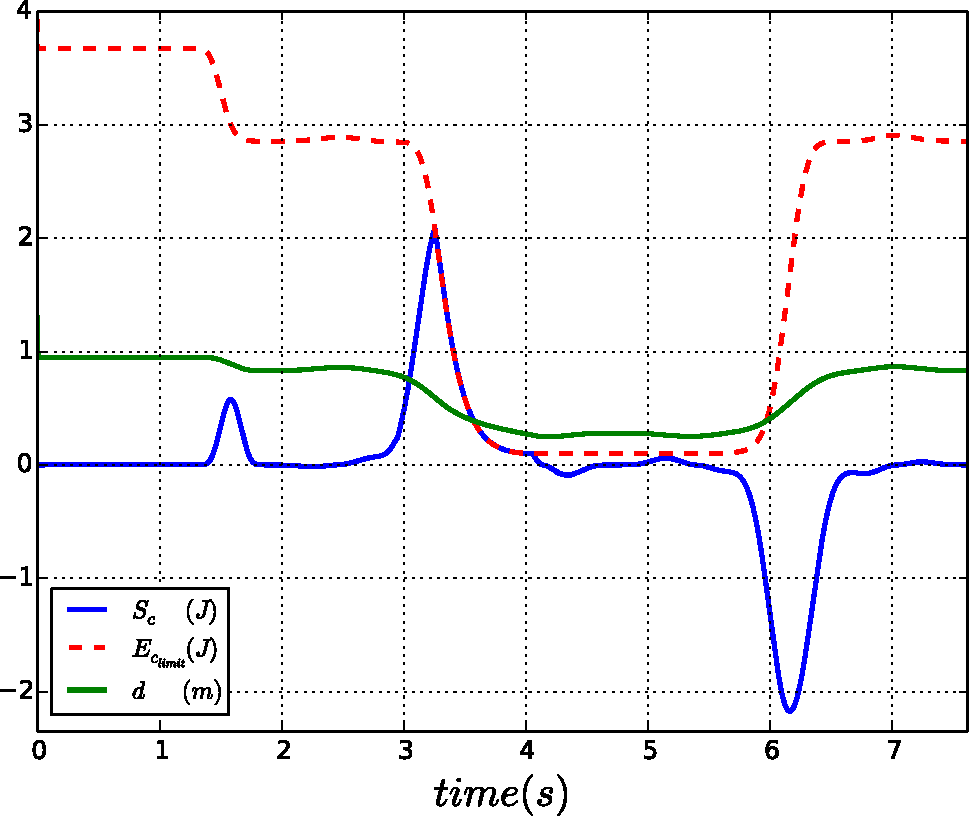
\includegraphics[width=0.80\columnwidth]{\figurepath/dist_ec_ecmax_plot1_2}}
\caption{Constrained kinetic energy of the robot expressed at its end-effector in the direction of a nearby considered obstacle (case $O_2$ in Fig.~\ref{fig:kuka_in_xde862301_a}).} 
\label{fig:dist_ec_ecmax_plot1_2}
\end{figure}
\begin{figure}[!htbp]
\centering
{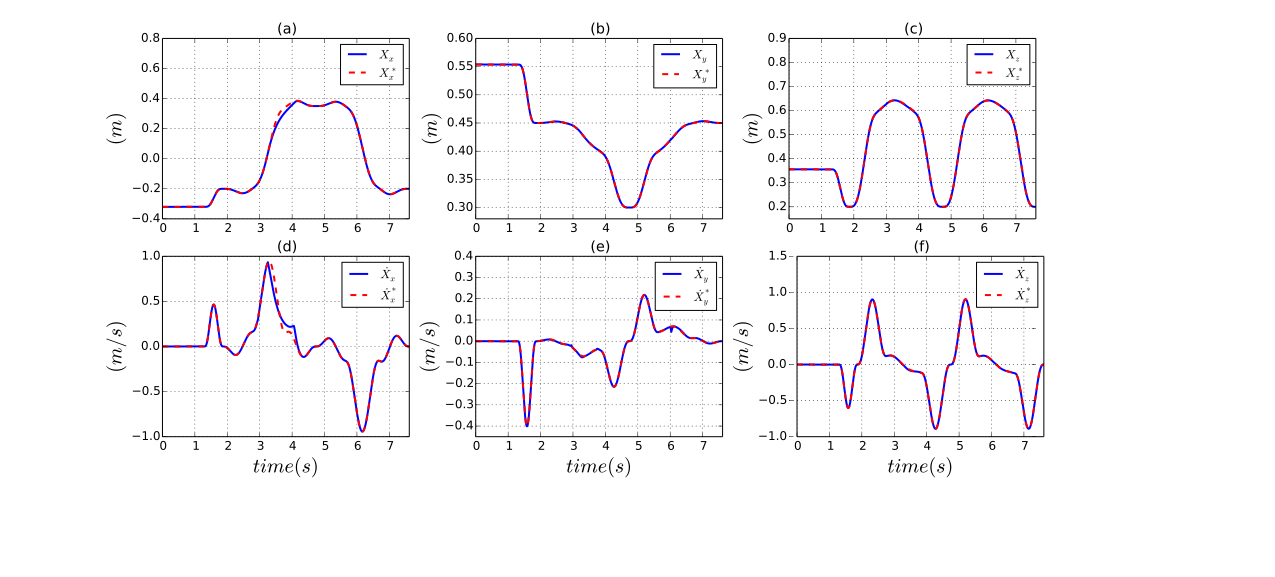
\includegraphics[width=1\columnwidth]{\figurepath/x_x_dot1_2}}
\caption{(a), (b) and (c) depict the real and desired position for the end-effector of the robot in Cartesian space as its kinetic energy is constrained. (d), (e) and (f) are the real and desired velocity for the end-effector as the system is submitted to the same constraint (case $O_2$ in Fig.~\ref{fig:kuka_in_xde862301_a}).} 
\label{fig:x_x_dot1_2}
\end{figure}
Fig.~\ref{fig:dist_ec_ecmax_plot1_2} shows how the kinetic energy related constraint is satisfied at every time-step; accordingly, a drop in the velocity of the end-effector of the robot can be observed in Fig.~\ref{fig:x_x_dot1_2}.d along the $\vect{x}$ axis component in Cartesian space. $\vect{x}$ here is the directing vector of the closest distance between the end-effector and obstacle $O_2$. At the activation of the constraint on kinetic energy, we highlight the resulting de-synchronisation between the real and desired position/velocity of the end-effector. 
%Caused by the constraint on kinetic energy, this de-synchronisation need
Caused by this same constraint, discontinuities in the actuation torque (mainly on $\tau_0$ and $\tau_2$) can also be seen in Fig.~\ref{fig:tau3_qddot!!!!}.a. \\
Because the kinetic energy related constraint is activated only one time-step before reaching the considered limit $E_{c_{limit}}$, high jerk performances ($10788~rad/s^3$ for joint $0$ as shown in Fig.~\ref{fig:tau3_qddot!!!!}.b) are needed to comply with this bound in such a small window of time. At the activation of such constraint, the braking movement needed to decrease the kinetic energy of the robot is induced by its actuators. As the braking capabilities (i.e., producible deceleration and jerk) of the system are not considered in the mathematical formulation of the constraint on kinetic energy (\ref{eq:Safe_constr_1}), incompatibility issues between this constraint and the hard-coded constraint on articular jerk (\ref{eq:cnt_lit_444}) may occur. In such case, coping with the maximum allowed amount of kinetic energy $E_{c_{limit}}$ may be impossible during only one control time-step, as it is  impossible to satisfy both constraints at the same time. The \textit{viability} of the state of the robot can then  be altered and the the LQP problem may become impossible to solve.
%\footnote{At the activation of the constraint on kinetic energy, a braking movement is induced by the actuators to decrease the kinetic energy of the robot. As the braking capabilities of the system are not considered in the mathematical formulation of this constraint (\ref{eq:Safe_constr_1}); Coping with the maximum allowed amount of kinetic energy $E_{c_{limit}}$ may be impossible during only one control time-step. Because of incompatibility issues between the constraint on kinetic energy and the hard-coded constraint on articular jerk (\ref{eq:cnt_lit_444}), the LQP problem can become impossible to solve (Both constraints cannot be satisfied at the same time). For this reason, constraints on articular jerk are removed whenever an energy related constraint is activated.} 
%\begin{figure}[!htbp]
%\centering
%{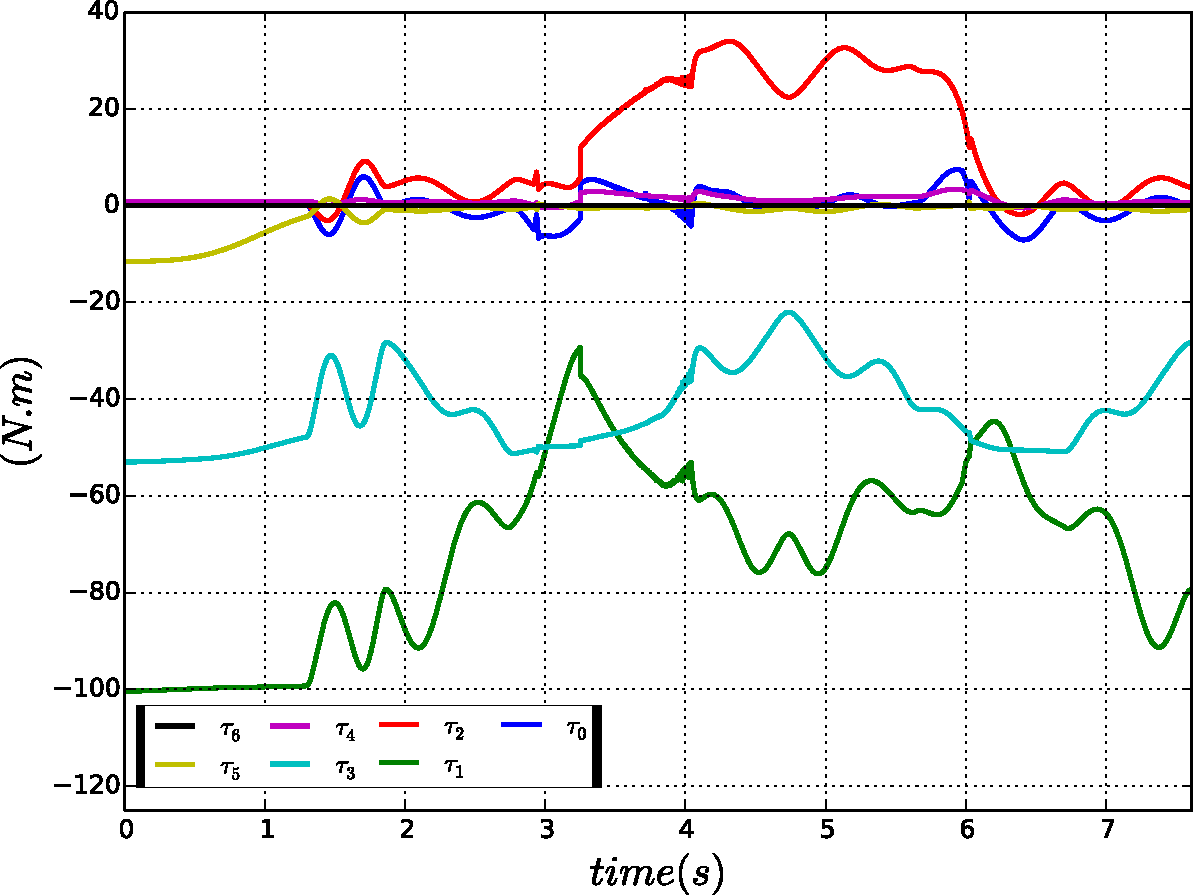
\includegraphics[width=0.8\columnwidth]{\figurepath/tau1_2!!!!}}
%\caption{1112} 
%\label{fig:tau1_2!!!!}
%\end{figure}
%\begin{figure}[!htbp]
%\centering
%{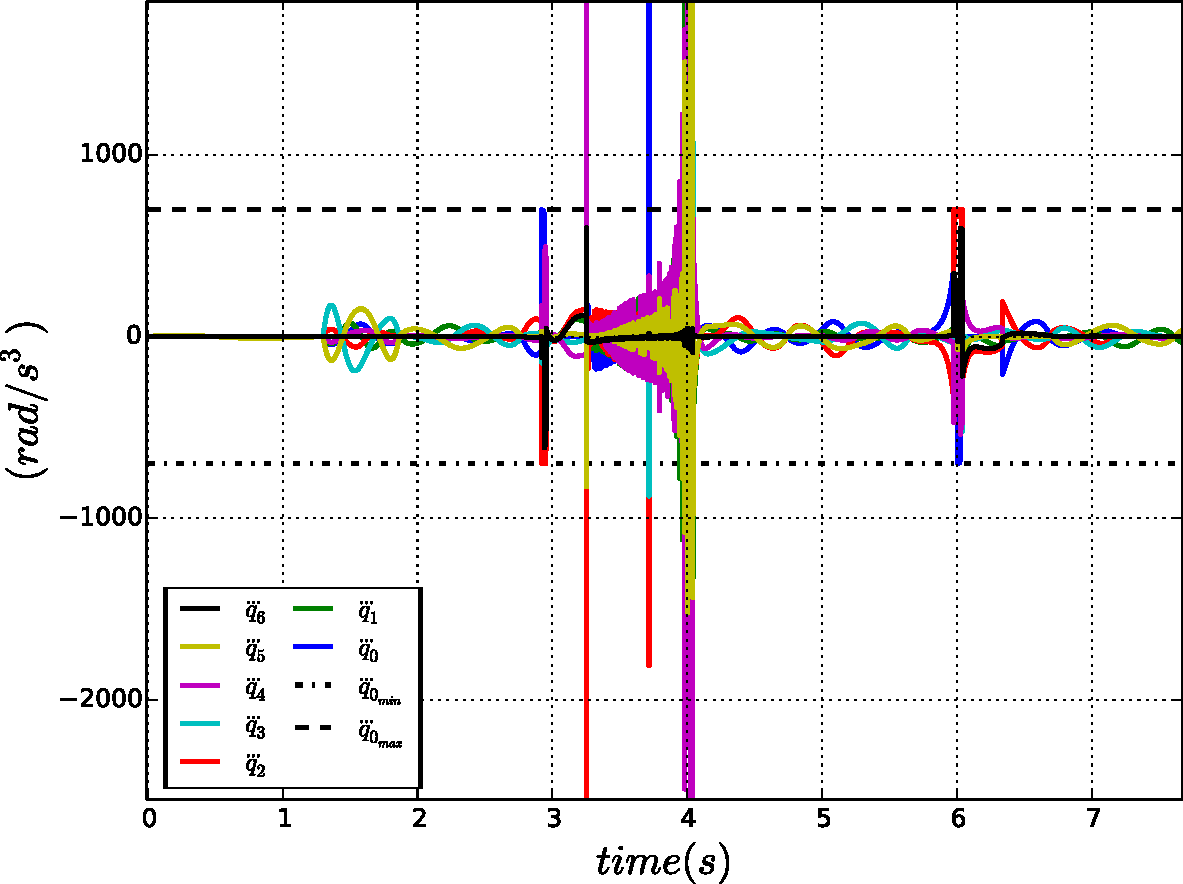
\includegraphics[width=0.9\columnwidth]{\figurepath/qdotdotdot_1_2!!!!}}
%\caption{12} 
%\label{fig:qdotdotdot_1_2!!!!}
%\end{figure}
\begin{figure}[!htbp]
\centering
{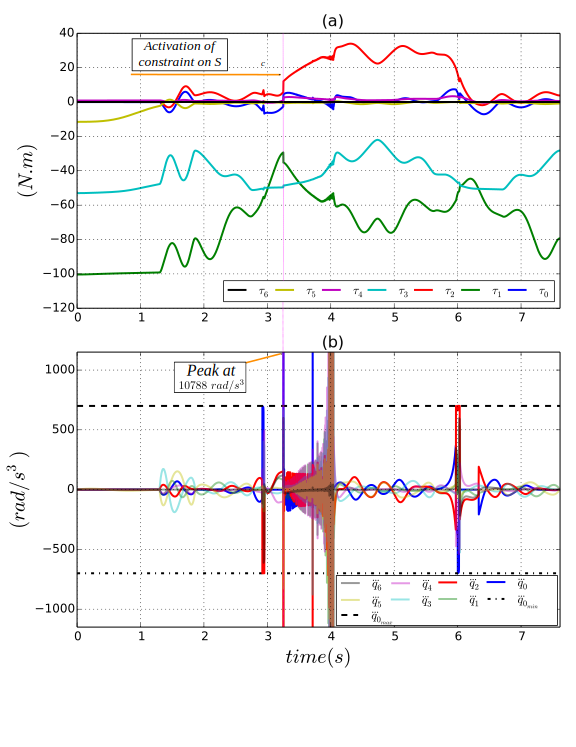
\includegraphics[width=0.89\columnwidth]{\figurepath/tau3_qddot!!!!}}
\caption{Generated articular torque and jerk as the constraint on the kinetic energy of the robot is activated (case $O_2$ in Fig.~\ref{fig:kuka_in_xde862301_a}).} 
\label{fig:tau3_qddot!!!!}
\end{figure}
On the other hand, chattering phenomena in both the articular torque and jerk, observed in Fig.~\ref{fig:tau3_qddot!!!!}, are caused by the discontinuities in the measured distance between the robot and the considered obstacle. This smallest distance between the end-effector of the robot and obstacle $O_2$ is computed in real-time and directly fed to the controller without being filtered. This actually mimics the quality of data that can be acquired using a real-life acquisition system like the Microsoft Kinect sensor in a real-life situation.
%\footnote{The smallest distance between the end-effector and the obstacle is computed in real-time. It is directly fed to the controller without any filtering. This actually mimics the kind of data that can be acquired with a real-life system (e.g., a Microsoft Kinect).} 
These discontinuities are reflected on the maximum allowed kinetic energy $E_{c_{limit}}$ and thus on the control input $\vect{\tau}_{|k}^{c}$. \\
Finally, as the kinetic energy of the robot is successfully constrained, the controller with its current configuration seems more appropriate for establishing safe physical interactions between the  robot and its environment. Physical contact is allowed in the following simulation.
%Mettre
%%%%%%%%%%%%%%%%%%%%%%%%%%SUBSECTION%%%%%%%%%%%%%%%%%%%%%%%%%%%%%
%%%%%%%%%%%%%%%%%%%%%%%%%%%%%%%%%%%%%%%%%%%%%%%%%%%%%%%%%%%%%%%%%
%%%%%%%%%%%%%%%%%%%%%%%%%%SUBSECTION%%%%%%%%%%%%%%%%%%%%%%%%%%%%%
\subsection{Scenario 3: obstacle intersecting with the trajectory of the robot and constraint on its kinetic energy} \label{subsec_inter_constr_Ec_classic}
In this scenario, obstacle $O_1$ intersects with the \circled{2}-\circled{3} segment of the pick and place movement. As the robot moves towards the wall, the first formulation of the kinetic energy related constraint (\ref{eq:Safe_constr_1}) is included in the configuration of the controller and used to reduce the kinetic energy the robotic manipulator displays before collision (see Fig.~\ref{fig:kuka_xde_obst_coll}). Articular inequality\footnote{Similarly to the previous simulation, the constraint on articular jerk is removed from the configuration of the controller whenever the constraint on kinetic energy (\ref{eq:Safe_constr_1}) is activated.} and equality constraints described in (\ref{eq:const_1_literature1}) and (\ref{eq:dyn_eq_aab}) are also considered. The parameters of the controller are fixed as: $E_{c_{safe}} = 0.05~J$, $K = 50~N$, $d_{safe} = 0.1~m$ and $d_{max} = 0.3~m$. 

Dissipated kinetic energy at collision is shown in Fig.~\ref{fig:dist_ec_ecmax_plot}.
%\begin{figure}[h]
%\centering
%{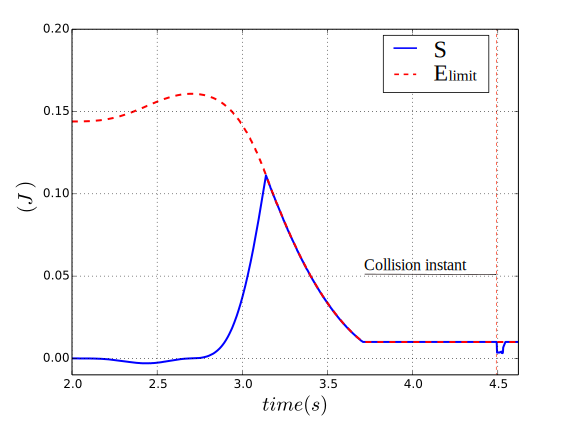
\includegraphics[width=0.6\columnwidth]{\figurepath/kE_wO_wC_wEc}}
%\caption{Dissipation of the constrained kinetic energy of the end-effector in the direction of the considered obstacle during a collision phase.} 
%\label{fig:kE_wO_wC_wEc}
%\end{figure}
%\begin{figure}[!htbp]
%\centering
%{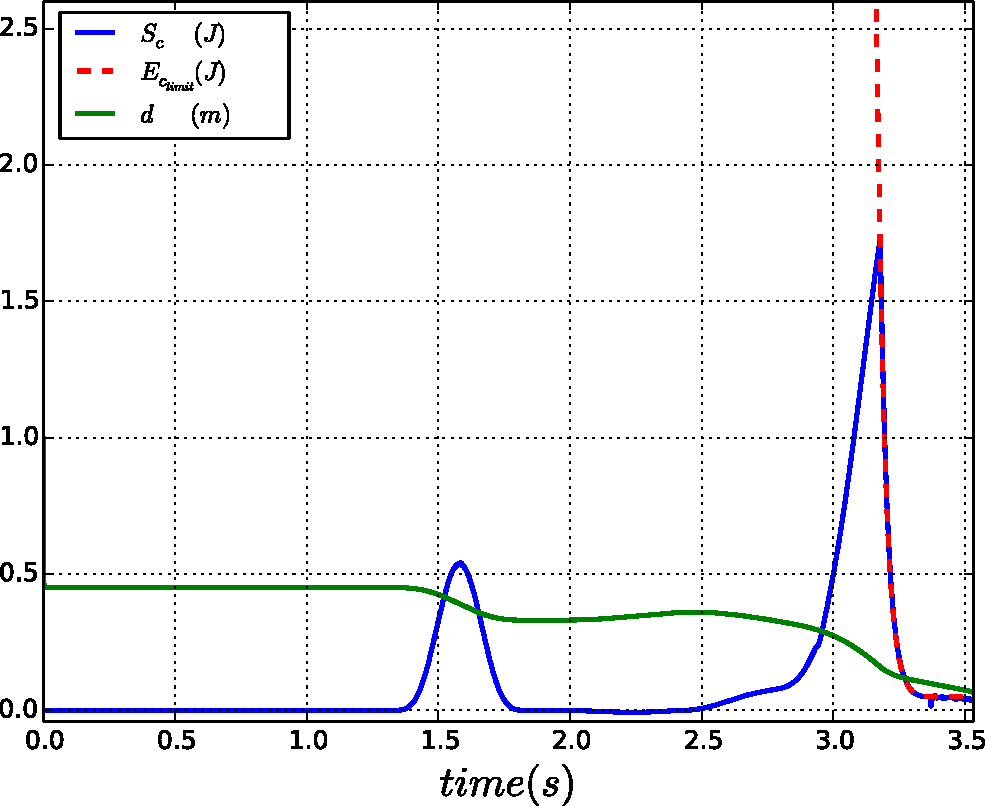
\includegraphics[width=0.8\columnwidth]{\figurepath/Dist_Ec_Ecmax_plot}}
%\caption{9} 
%\label{fig:Dist_Ec_Ecmax_plot}
%\end{figure}
\begin{figure}[!htbp]
\centering
{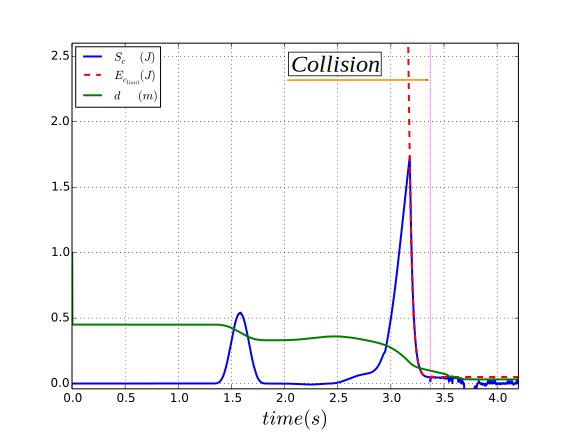
\includegraphics[width=0.82\columnwidth]{\figurepath/dist_ec_ecmax_plot}}
\caption{Constrained kinetic energy of the robot expressed at the level of its end-effector in the direction of the collided obstacle (case $O_1$ in Fig.~\ref{fig:kuka_in_xde862301_a}).} 
\label{fig:dist_ec_ecmax_plot}
\end{figure}
Compared to the collision case where the kinetic energy of the robot is not constrained (as in Fig.~\ref{fig:ec_obst3!!!!}), we underline the benefit of using the kinetic energy based safety criterion introduced in (\ref{eq:Ec_constr_first}). Indeed, at collision, the amount of dissipated kinetic energy ($0.035~J$) when this latter is initially constrained is far less than its amount if the introduced constraint on kinetic energy is not included in the configuration of the controller ($1.66~J$). Accordingly,
the resulting impact force shown in Fig.~\ref{fig:ep__f_tau75_!!!!}.a is largely reduced: $86~N$ compared to the collision force when the kinetic energy of the robot is not pre-constrained ($551~N$ as shown in Fig.~\ref{fig:ep__f_tau_!!!!}.b). Using the kinetic energy related constraint (\ref{eq:Safe_constr_1}), the ability to saturate the kinetic energy of the robot at a safe limit before collision enables a safer physical-contact establishment/impact between the robot and its environment. \\
% \begin{figure}[!htbp]
%\centering
%{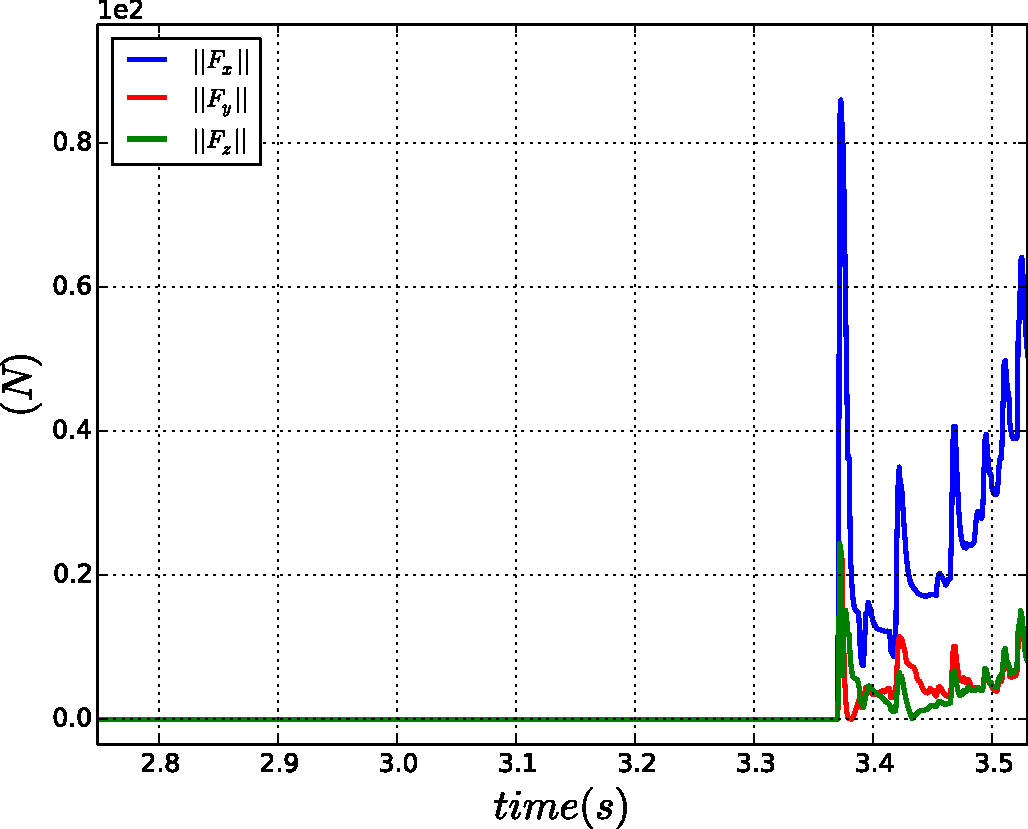
\includegraphics[width=0.99\columnwidth]{\figurepath/force_sensor22}}
%\caption{10} 
%\label{fig:force_sensor22}
%\end{figure}
 \begin{figure}[!htbp]
\centering
{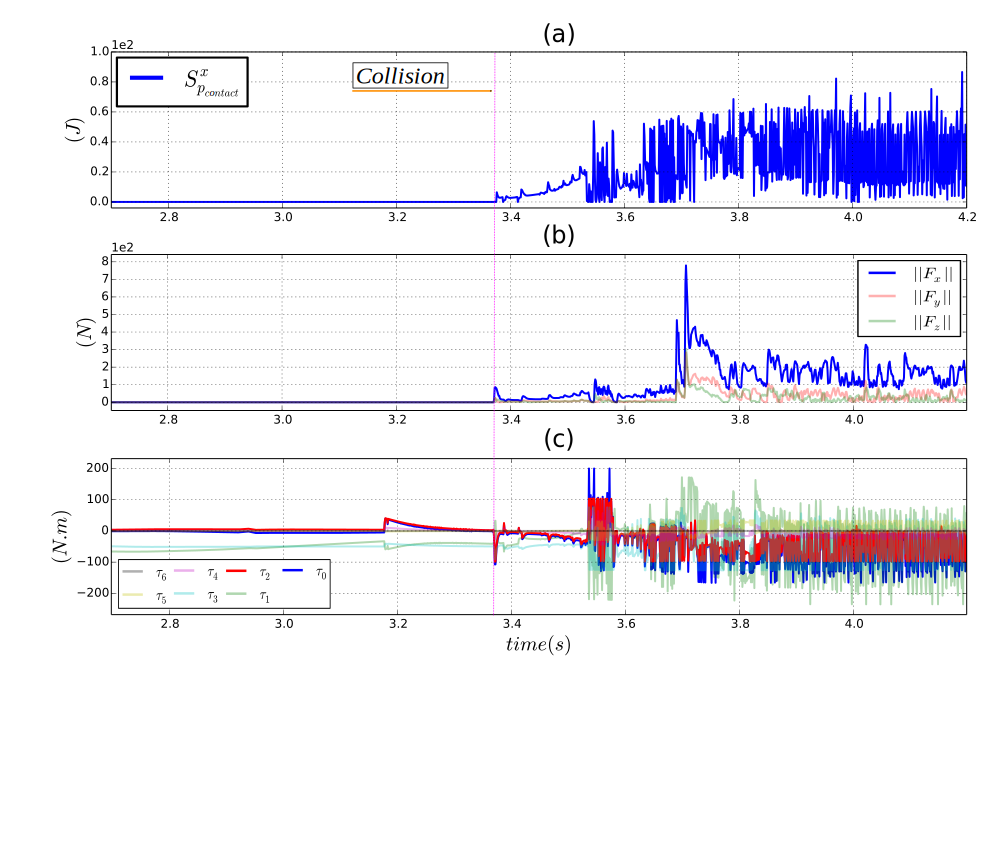
\includegraphics[width=1\columnwidth]{\figurepath/ep__f_tau75_!!!!}}
\caption{(a) \textit{Potential energy} stored in the controller of the robot during physical contact along the $\vect{x}$ axis in Cartesian space. (b) Corresponding contact forces along the $\vect{x}$, $\vect{y}$ and $\vect{z}$ axis in Cartesian space. (c) Actuation torques during physical contact with the considered obstacle (case $O_1$ in Fig.~\ref{fig:kuka_in_xde862301_a}).} 
\label{fig:ep__f_tau75_!!!!}
\end{figure}
On the other hand, as in scenario~1, after  the establishment of physical-contact, \textit{potential energy} starts increasing in the controller of the robot (see Fig.~\ref{fig:ep__f_tau75_!!!!}.a). Consequently, as illustrated in Fig.~\ref{fig:ep__f_tau75_!!!!}.b, the resulting contact force also increases to reach an average value of $100~N$, which may be potentially harmful for any human-operator within the workspace of the robot. Actuation torques are shown in Fig.~\ref{fig:ep__f_tau75_!!!!}.

In the current scenario, even after the establishment of physical contact, the constraint on kinetic energy is never removed from the configuration of the controller. However, as it depends on the real-time distance $d$ between the end-effector of the robot and the considered obstacle $O_1$, this constraint may be released is case $d$ is equal to zero. \\
To summarize, in this scenario, the configuration of the controller that accounts for the constraint on the kinetic energy of the robot is considered more suitable for physical contact establishment/collision, compared to the case where the kinetic energy related constraint is not included in the control scheme. However, to ensure safety even during the physical contact phase, the \textit{potential energy} that accumulates in the controller of the robot from which the hazardous contact force is derived must also be constrained. This constraint is considered in the scenario of the following simulation.
\begin{figure}[!htbp]
\centering
{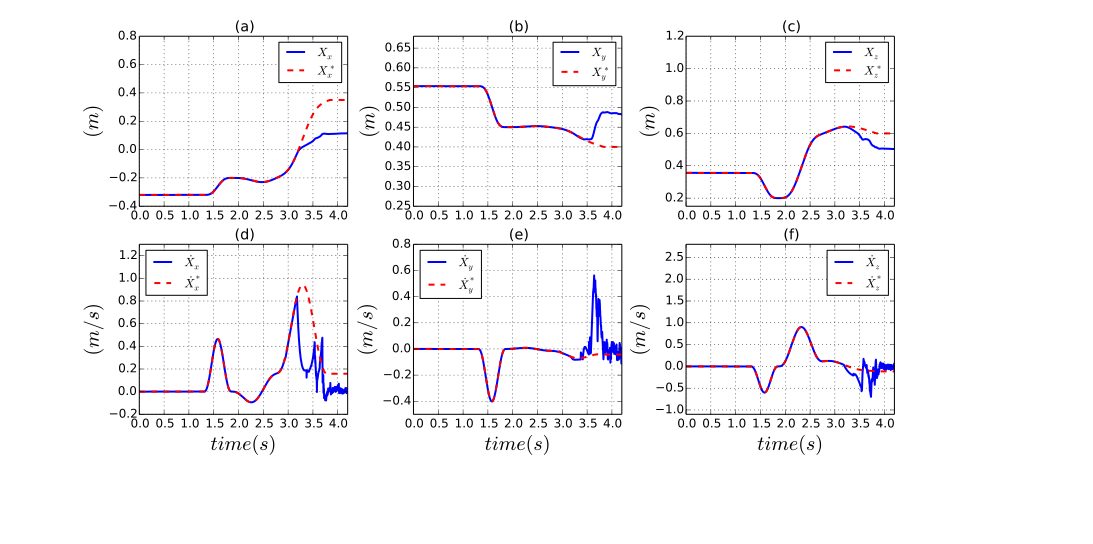
\includegraphics[width=1\columnwidth]{\figurepath/x_x_dot4_com}}
\caption{(a), (b) and (c) depict the real and desired position for the end-effector of the robot in Cartesian space as its kinetic energy is constrained. (d), (e) and (f) are the real and desired velocity for the end-effector as the robot is submitted to the same constraint (case $O_1$ in Fig.~\ref{fig:kuka_in_xde862301_a}).} 
\label{fig:x_x_dot4_com}
\end{figure}
%\begin{figure}[!htbp]
%\centering
%{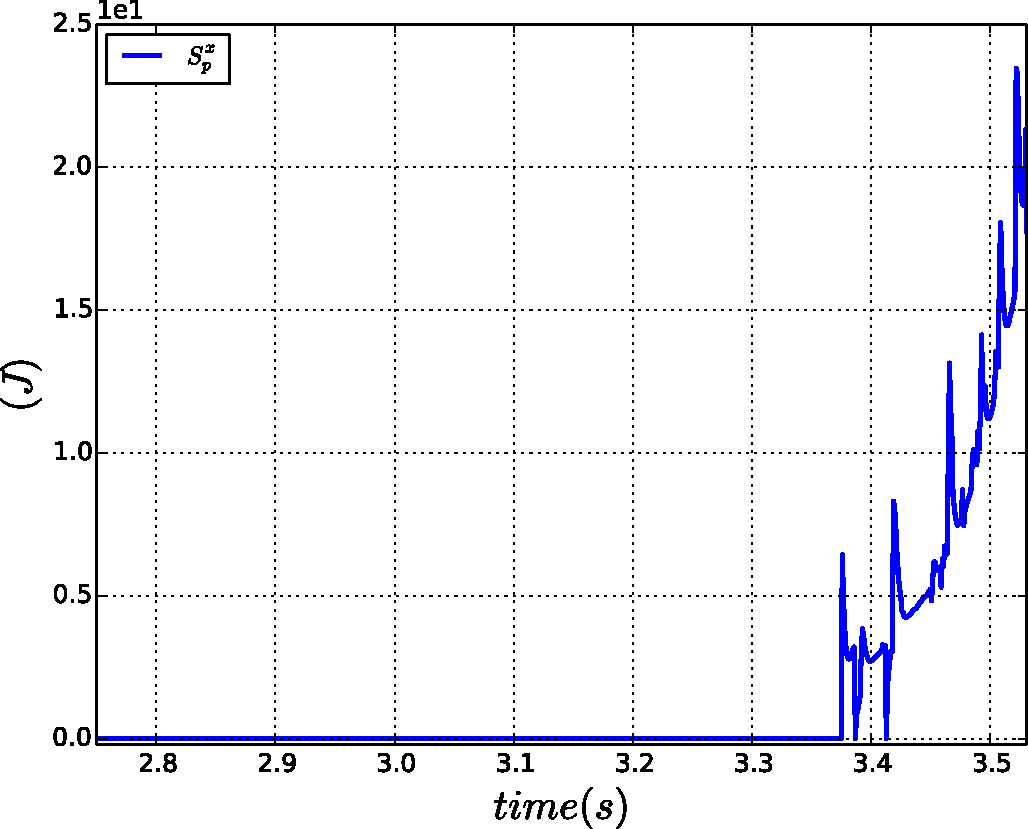
\includegraphics[width=0.8\columnwidth]{\figurepath/ep_contact_selon_x_seul_!!!!}}
%\caption{12} 
%\label{fig:ep_contact_selon_x_seul_!!!!}
%\end{figure}
%\clearpage
%\begin{figure}[!htbp]
%\centering
%{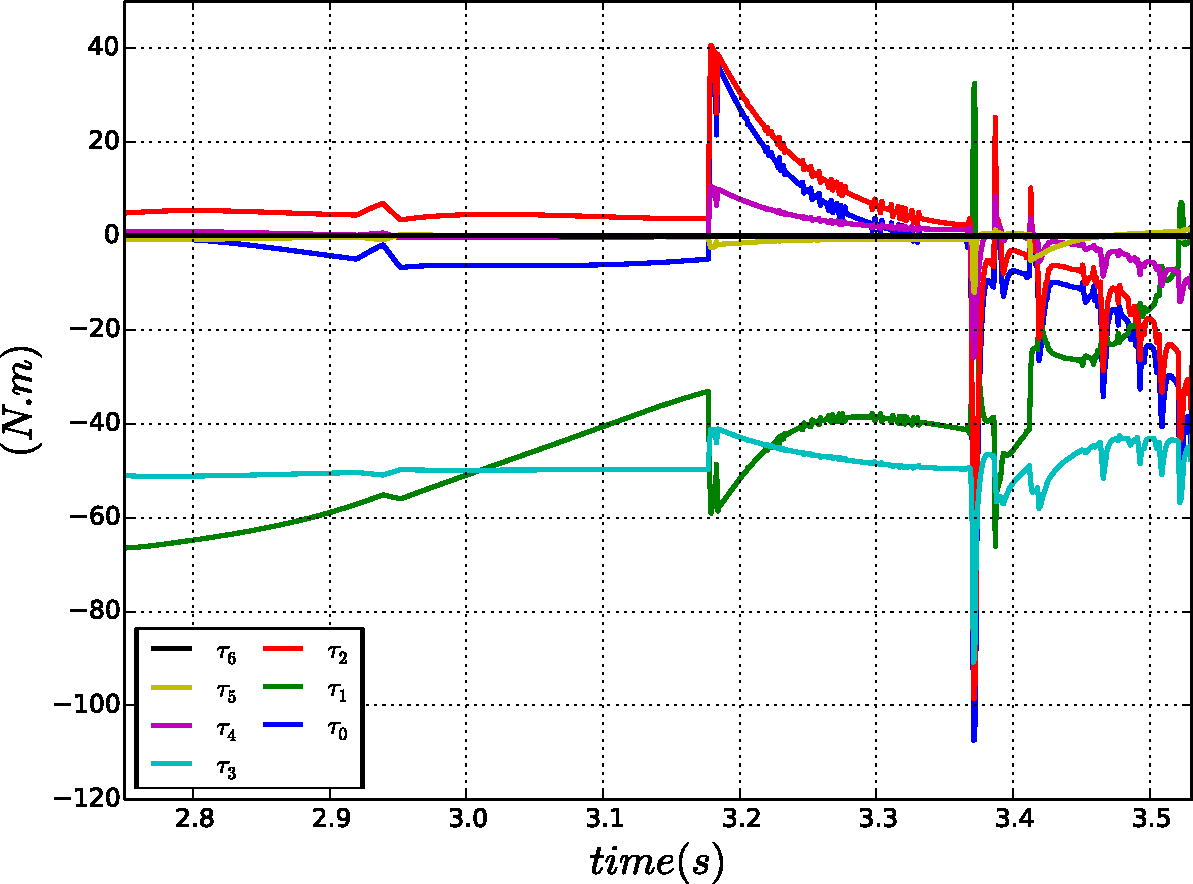
\includegraphics[width=0.8\columnwidth]{\figurepath/tau22}}
%\caption{15} 
%\label{fig:tau22}
%\end{figure}
%%%%%%%%%%%%%%%%%%%%%%%%%%SUBSECTION%%%%%%%%%%%%%%%%%%%%%%%%%%%%%
%%%%%%%%%%%%%%%%%%%%%%%%%%%%%%%%%%%%%%%%%%%%%%%%%%%%%%%%%%%%%%%%%
%%%%%%%%%%%%%%%%%%%%%%%%%%SUBSECTION%%%%%%%%%%%%%%%%%%%%%%%%%%%%%
\subsection{Scenario 4: obstacle intersecting the trajectory of the robot and constraints on its kinetic and \textit{potential} energies}
Similarly to the previous scenario, the wall intersects with the \circled{2}-\circled{3} segment of the pick and place movement. As the robot moves, the second formulation of the constraint on kinetic energy (\ref{eq:Safe_constr_2}) is included in the configuration of the controller and used to limit the amount of kinetic energy the robotic manipulator deploys in the direction of obstacle $O_1$. This constraint also depends on the real-time closest distance between the wall and the end-effector of the robot. After the establishment of physical-contact, without removing the constraint on kinetic energy(\ref{eq:Safe_constr_2}), the constraint (\ref{eq:eqAA}) is added to the controller and used to saturate the amount of \textit{potential energy} that accumulates in the controller of the robot. Articular inequality\footnote{Similarly to the previous case, the constraint on articular jerk is removed from the controller whenever an energy related constraint (kinetic (\ref{eq:Safe_constr_2}) or  potential (\ref{eq:Safe_constr_4_x_axis})) is activated.} and equality constraints described in (\ref{eq:const_1_literature1}) and (\ref{eq:dyn_eq_aab}) are also considered in the control scheme. The parameters of the controller are fixed as: $E_{c_{safe}} = 0.05~J$, $K = 50~N$, $d_{safe} = 0.1~m$, $d_{max} = 0.3~m$ and $E_{p_{safe}}^{x} = 0.1~J$. During the physical-contact phase, contact forces applied by the robot to the wall are \textit{mainly} along the $\vect{x}$ axis. Consequently, only the \textit{potential energy} along this vector is constrained. 

Dissipated kinetic energy at collision is shown in Fig.~\ref{fig:dist_ec_ecmax_plot55}. As it is  pre-constrained, only $0.035~J$ of kinetic energy are dissipated at collision, resulting into an impact force of $85~N$ (see Fig.~\ref{fig:ep__f_tau65_!!!!}.b).
\begin{figure}[!htbp]
\centering
{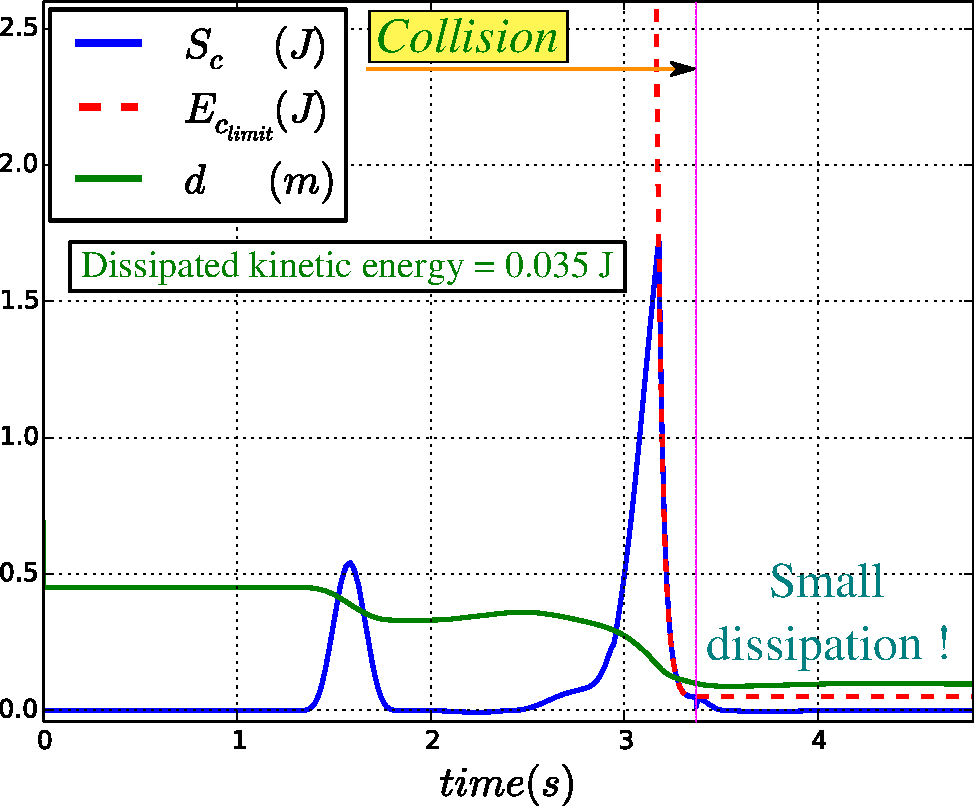
\includegraphics[width=0.75\columnwidth]{\figurepath/dist_ec_ecmax_plot55}}
\caption{Constrained kinetic energy of the robot expressed at the level of its end-effector in the direction of the collided obstacle (case $O_1$ in Fig.~\ref{fig:kuka_in_xde862301_a}).} 
\label{fig:dist_ec_ecmax_plot55}
\end{figure}
%\begin{figure}[!htbp]
%\centering
%{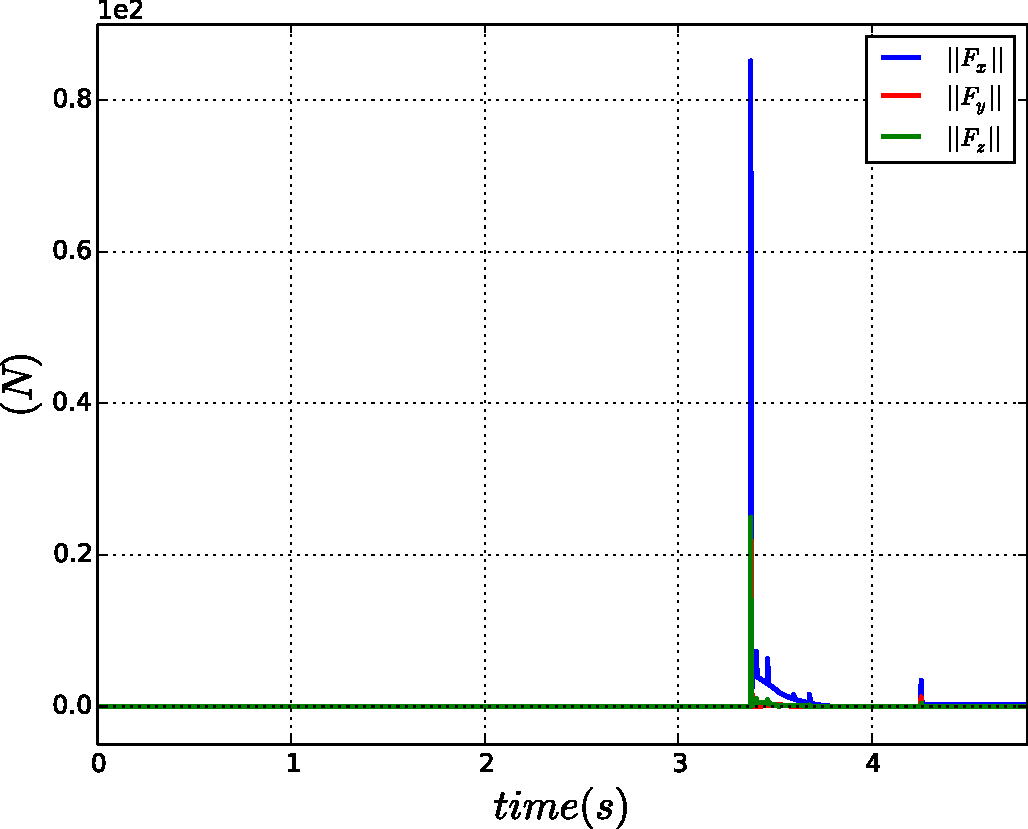
\includegraphics[width=0.8\columnwidth]{\figurepath/force_sensor255}}
%\caption{10} 
%\label{fig:force_sensor255}
%\end{figure}
\begin{figure}[!htbp]
\centering
{
\includegraphics[width=0.90\columnwidth]{\figurepath/ep__f_tau65_!!!!}}
\caption{(a) Constrained \textit{potential energy} stored in the controller of the robot during physical contact along the $\vect{x}$ axis in Cartesian space. (b) Corresponding contact forces along the $\vect{x}$, $\vect{y}$ and $\vect{z}$ axis in Cartesian space. (c) Actuation torques during the physical contact with the considered obstacle (case $O_1$ in Fig.~\ref{fig:kuka_in_xde862301_a}).} 
\label{fig:ep__f_tau65_!!!!}
\end{figure}
As shown in Fig.~\ref{fig:dist_ec_ecmax_plot55}, the second formulation of the constraint on kinetic energy (\ref{eq:Safe_constr_2}) is satisfied at every time-step, exactly the same as when the first formulation (\ref{eq:Safe_constr_1}) is used (see subsection \ref{subsec_inter_constr_Ec_classic}). On the other hand, Fig.~\ref{fig:ep__f_tau65_!!!!}.a shows how the constraint on the \textit{potential energy} that accumulates in the controller of the robot during physical-contact is also satisfied at every time-step.
%\begin{figure}[!htbp]
%\centering
%{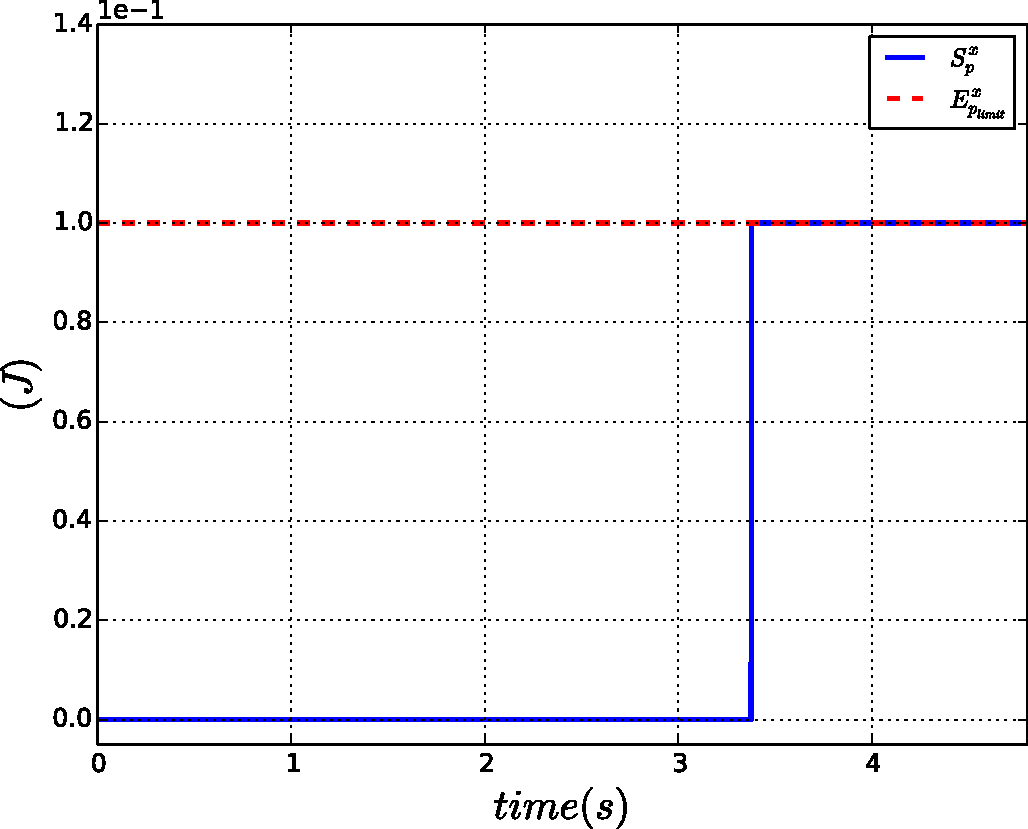
\includegraphics[width=0.8\columnwidth]{\figurepath/ep_contact_selon_x_seul_!!!!55}}
%\caption{11} 
%\label{fig:ep_contact_selon_x_seul_!!!!55}
%\end{figure}
Because this \textit{potential energy} is saturated at a constant value $0.1~J$, the contact force derived from it decreases over time to reach $0~N$ (see Fig.~\ref{fig:ep__f_tau65_!!!!}.b) as the Cartesian tracking error between the real and desired positions for the end-effector of the robot increases. This finally causes the release of physical contact between the robot and the wall intersecting with its trajectory. When using the current configuration of the controller, if any physical-contact is established between the robotic manipulator and a human-operator in its workspace, the robot can easily and safely be moved or pushed away. \textit{The decrease} in the resulting contact force while the error between the desired and real positions for the end-effector of the robot \textit{increases} is actually exactly the inverse of what happens when the \textit{potential energy} related constraint is not included in the controller of the robot. In such case, tracking errors increase, \textit{potential energy} accumulates in the controller and accordingly hazardous contact forces (as shown in scenario~1).\\ Fig.~\ref{fig:ep__f_tau65_!!!!}.c shows the actuation torques of joint $0$ and joint $2$ as a peak is created when the braking phase implicitly induced to cope with the kinetic energy related constraint is engaged. 
%\begin{figure}[!htbp]
%\centering
%{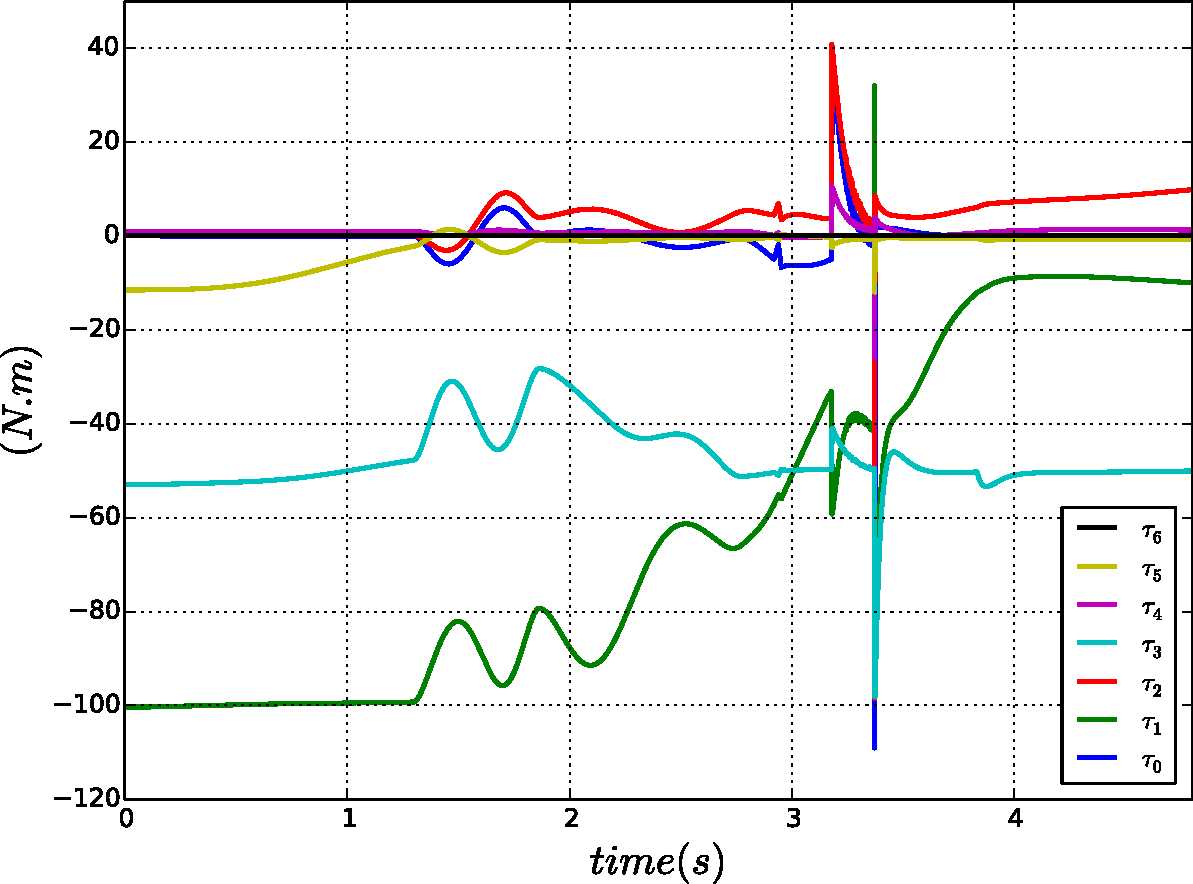
\includegraphics[width=0.8\columnwidth]{\figurepath/tau2555}}
%\caption{12} 
%\label{fig:tau2555}
%\end{figure}
%%%%%%%%%%%%%%%%%%%%%%%%%%SUBSECTION%%%%%%%%%%%%%%%%%%%%%%%%%%%%%
%%%%%%%%%%%%%%%%%%%%%%%%%%%%%%%%%%%%%%%%%%%%%%%%%%%%%%%%%%%%%%%%%
%%%%%%%%%%%%%%%%%%%%%%%%%%SUBSECTION%%%%%%%%%%%%%%%%%%%%%%%%%%%%%
\subsection{Scenario 5: obstacle intersecting with the trajectory of the robot and constraint on its task energy profile}
In this scenario, obstacle $O_1$ also intersects with the \circled{2}-\circled{3} segment of the pick and place movement. During the movement of the robot, its energy profile  (described in Section~\ref{subsec:Task_energy_profile}) related to the accomplished pick and place task is constrained using (\ref{eq:Safe_constr_3_axis}). The kinetic energy of the robot is not constrained and the articular inequality and equality constraints respectively described in (\ref{eq:const_1_literature1}) and (\ref{eq:dyn_eq_aab}) are also included in the configuration of the controller. As shown in Fig.~\ref{fig:energy_profile}, based on the measured energy profiles along the $\vect{x}$, $\vect{y}$ and $\vect{z}$ axis, the  parameters of the controller are fixed as: $E_{p_{profile}}^{x}+\epsilon_{E_p}^{x} = 0.01~J$, $E_{p_{profile}}^{y}+\epsilon_{E_p}^{y} = 0.0045~J$ and $E_{p_{profile}}^{z}+\epsilon_{E_p}^{z} = 0.015~J$. With $\epsilon_{E_p}^{x}$, $\epsilon_{E_p}^{y}$ and $\epsilon_{E_p}^{z}$ used to compensate the repeatability related variations on the controller's \textit{potential energy} needed to accomplish the pick and place task.
%\footnote{According to the measured energy profiles in Fig.~\ref{fig:energy_profile}.b, Fig.~\ref{fig:energy_profile}.c and Fig.~\ref{fig:energy_profile}.d, \epsilon_{E_p}^{x}}. \\

As can be seen in Fig.~\ref{fig:x_x_dot454}, during the pre-collision phase, the tracking performances of the controller are not altered by the \textit{task energy profile} related constraint. Indeed, during the \textit{free} movement of the robot, this constraint is never activated. The desired position, orientation and velocity for the end-effector are properly tracked, exactly the same as if this constraint is not included in the control scheme. \\
At collision, the impact of the robot with the wall is not detected and the desired position (also the velocity) for the end-effector starts diverging from its real value. Consequently, the \textit{potential energy} stored in the controller starts to increase and triggers the activation of the constraint on the \textit{task energy profile}. During physical contact, this constraint behaves exactly the same as (\ref{eq:Safe_constr_4_3_axis54}). According to Fig.~\ref{fig:ep_profil_xyz_futur_with_recnstruted6}, the \textit{potential energy} related constraint is successfully satisfied along the $\vect{x}$, $\vect{y}$ and $\vect{z}$ axis.
The peak of \textit{potential energy} along the $\vect{x}$ axis at collision is however caused by the induced impact force. \\
Fig.~\ref{fig:ec__f_tau65_grand_!!!!}.a shows how $1.66~J$ of kinetic energy are dissipated at impact. Fig.~\ref{fig:ec__f_tau65_grand_!!!!}.b depicts the resulting collision  and contact force: $551~N$ are induced at the first impact. The other collision peaks are caused by collisions between other parts of the robot and the wall. During physical contact, the constraint on the controller's accumulated \textit{potential energy} when expressed at the level of the end-effector, does not prevent the movement of other \textit{free} parts of the body of the robot.  \\ 
Thanks to the constraint on the \textit{task energy profile} that has been included in the configuration of the controller, the resulting contact force is also reduced and it decreases over time as the desired and real positions for the end-effector diverge. The robot at this stage is compliant and can easily and safely be moved by a human-operator. The actuation torque generated during this simulation is shown in Fig.~\ref{fig:ec__f_tau65_grand_!!!!}.
\begin{figure}[!htbp]
\centering
{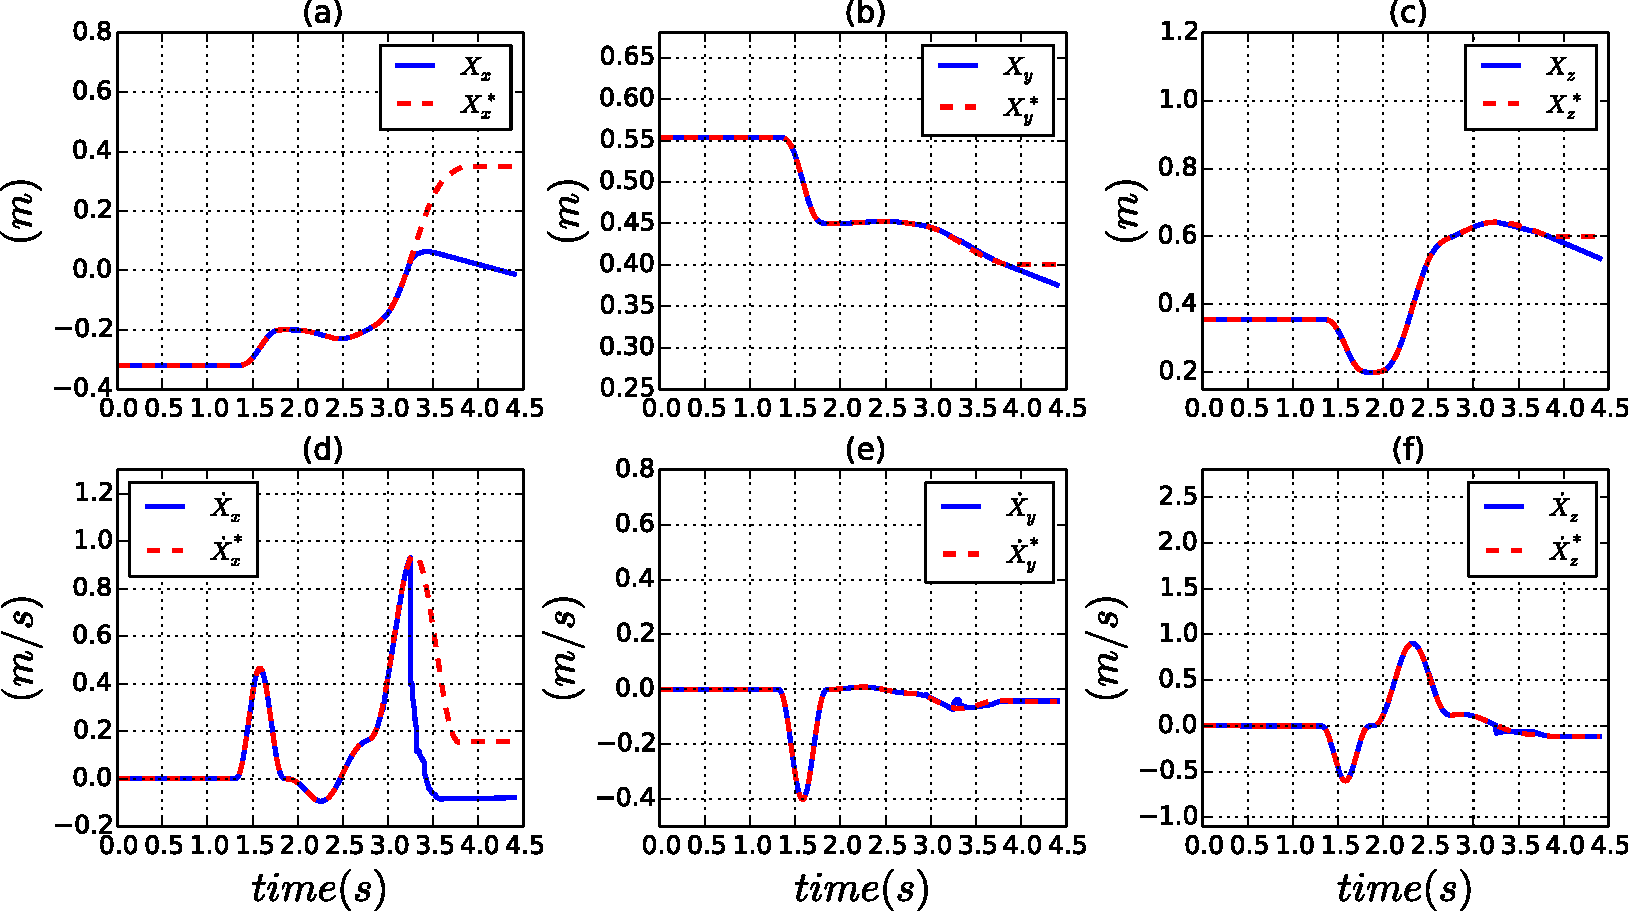
\includegraphics[width=1\columnwidth]{\figurepath/x_x_dot454}}
\caption{(a), (b) and (c) depict the real and desired position for the end-effector of the robot in Cartesian space as its task energy profile is constrained. (d), (e) and (f) are the real and desired velocity for the end-effector as the robot is submitted to the same constraint (case $O_1$ in Fig.~\ref{fig:kuka_in_xde862301_a}).} 
\label{fig:x_x_dot454}
\end{figure}
\begin{figure}[!htbp]
\centering
{\includegraphics[width=0.90\columnwidth]{\figurepath/ep_profil_xyz_futur_with_recnstruted6}}
\caption{Constrained energy profile for the pick and place task along the $\vect{x}$, $\vect{y}$ and $\vect{z}$ axis in Cartesian space.} 
\label{fig:ep_profil_xyz_futur_with_recnstruted6}
\end{figure}
\begin{figure}[!htbp]
\centering
{\includegraphics[width=0.90\columnwidth]{\figurepath/ec__f_tau65_grand_!!!!}}
\caption{(a) The kinetic energy of the robot expressed at the level of its end-effector as it physically interacts with the nearby obstacle (case $O_1$ in Fig.~\ref{fig:kuka_in_xde862301_a}). (b) Corresponding contact forces along the $\vect{x}$, $\vect{y}$ and $\vect{z}$ axis in Cartesian space. (c) Actuation torques during physical contact.} 
\label{fig:ec__f_tau65_grand_!!!!}
\end{figure}
%\begin{figure}[!htbp]
%\centering
%{\includegraphics[width=0.8\columnwidth]{\figurepath/ec_obst6}}
%\caption{9} 
%\label{fig:ec_obst6}
%\end{figure}
%\begin{figure}[!htbp]
%\centering
%{\includegraphics[width=0.8\columnwidth]{\figurepath/force_sensor6}}
%\caption{11} 
%\label{fig:force_sensor6}
%\end{figure}
%\begin{figure}[!htbp]\centering
%{\includegraphics[width=0.8\columnwidth]{\figurepath/tau26}}
%\caption{12} 
%\label{fig:tau26}
%\end{figure}
%
%%%%%%%%%%%%%%%%%%%%%%%%%%%%%%%%%%%%%%%%%%%%%%%%%%%%%%%%%%
%          %Experimental results REAL ROBOT%
%%%%%%%%%%%%%%%%%%%%%%%%%%%%%%%%%%%%%%%%%%%%%%%%%%%%%%%%%%
\section{Conclusion}
\label{sec:safety1conclusion}
%The energy based safety indicators presented in this chapter allow a continuously safe human-robot interaction.  It allows the robotic system to adapt its dynamic behaviour from the approach of the human operator to the establishment of physical contact. Contact and impact forces are modulated all along the interaction process and the contact enabling/disabling transition is smoothed thanks to the universality of the energetic formulation. 
%
%The energy based safety indicator proposed and validated in this chapter holds a great
%potential for human/robot collaboration tasks. Indeed, energy is a universal component
%that can describe several physical phenomena linked to the physical interaction process.
%Velocity, inertia and also contact forces can all be expressed and modulated with this
%same quantity. Using the presented control framework and the introduced energy based
%criterion, the robot has been proven capable of producing different behaviours towards a
%nearby considered obstacle just by acting on physically meaningful control parameters.
%During its motion, at every time-step, the kinetic energy of the end-effector is controlled.
%If a collision occurs or contact with the environment is desired, the dissipated energy
%is modulated to smooth the interaction process and guarantee safety for both the robot
%and the obstacle. Enabling/disabling contact and stopping the robot at a desired distance
%from the obstacle are different behaviours that can be obtained using the same controller.
Energy-based safety indicators proposed and validated in this chapter hold a great potential for human-robot collaboration tasks. Indeed, energy is a universal component that can describe all the physical phenomena occurring during an interaction between the robot and its environment. Velocity, inertia, impact and also contact forces can all be expressed and modulated with this same property. Using the presented control framework and the introduced energy-based criteria, it has been proven possible to control the energy of the robot. During its movement and at every time-step, the kinetic energy of the robot can be tracked then saturated to meet the imposed safety criteria needed for a safe establishment of physical contact. Dissipated kinetic energy at impact is reduced and the induced collision force is harmless. \\
After the establishment of physical contact, contact forces can also be saturated by constraining the \textit{potential energy} that accumulates in the controller of the robot. In case of a human-robot interaction, the robot can easily and safely be pushed and moved as needed. 
%As the energy of the robot can be controlled, release of physical-contact has also been made safer as the hazardous transformation of the controller's potential energy into kinetic one is prevented.
In addition to the kinetic and \textit{potential energy} related constraints, the constraint on kinetic energy is reformulated as a constraint on the \textit{potential energy} instantaneously held in the controller of the robot. Consequently, the amount of \textit{potential energy} \textit{injected} in the controller of the robot at every time-step can be used as a safety indicator for both the pre and post collision phases. \\
Moreover, the concept or \textit{task energy profile} has been introduced and used to synthesise a low-level security layer to deal with non-deliberate or undetected collisions between the robot and its environment. The proposed constraint on the \textit{task energy profile} prevents the robot from accumulating any additional amount of energy than what it needs to perform its main task. This has the effect of preventing any harmful contact forces as the controller of the robot is restrained from ``\textit{loading}'' any additional amount of \textit{potential energy} in case a physical-contact with the environment is established. \\
%Moreover, the concept or \textit{task energy profile} has been introduced and used to synthesise a low-level security layer to deal with non-deliberate or undetected collisions between the robot and its environment. The proposed constraint on the \textit{task energy profile} allows the robot to produce only the needed amount of energy to perform its main task. This prevents any harmful contact forces as the controller of the robot is restrained from ``loading'' any additional amount of potential energy in case a physical-contact with its environment is established. \\
Constraints on kinetic and potential energies are expressed in Cartesian space and are non-linearly related to the instantaneous state $S_{|k}=\{\vect{q}_{|k}, \vect{\dot{q}}_{|k}, \vect{\ddot{q}}_{|k}, \vect{\dddot{q}}_{|k}\}$ of the robot in articular space. Such constraints are of type 6 (see table \ref{my-label} in Chapter~\ref{chap:Constrcomp}) and due to how these are currently formulated, the energy related constraints are activated only one time-step before reaching their respective limits, which may render the control problem impossible to solve. Indeed, for example, the robotic manipulator may not have sufficient \textit{braking} capabilities to react and cope with an imposed kinetic energy limit $E_{c_{limit}}$ within only one control time-step. Its braking capabilities, namely: producible articular deceleration $[\vect{\ddot{q}}_m, \vect{\ddot{q}}_M]$ and jerk $[\vect{\dddot{q}}_m, \vect{\dddot{q}}_M]$ should therefore imperatively be part of the formulation of these constraints. With such new formulations, the energy related constraints can be activated at the right moment in order to guarantee the preservation of the \textit{viability} of the state of the robot. Otherwise, \textit{constraints incompatibility} issues as tackled Chapter~\ref{chap:Constrcomp} may appear and it may be impossible to implement these constraints on a real robot which actuators have limited dynamic capabilities. In the following chapter, the introduced energy related constraints are tested on a real KUKA LWR4 robotic manipulator as it physically interacts with a human-operator.
%the robot has been proven
%capable of producing different behaviours towards a nearby
%considered obstacle just by acting on physically meaningful
%control parameters. During its motion, at every time-step,
%the kinetic energy of the end-effector is controlled. If a
%collision occurs or contact with the environment is desired,
%the dissipated energy is modulated to smooth the interaction
%process and guarantee safety for both the robot and the
%obstacle. Enabling/disabling contact and stopping the robot at
%a desired distance from the obstacle are different behaviours
%that can be obtained using the same controller.






